\documentclass[twoside]{book}

% Packages required by doxygen
\usepackage{fixltx2e}
\usepackage{calc}
\usepackage{doxygen}
\usepackage[export]{adjustbox} % also loads graphicx
\usepackage{graphicx}
\usepackage[utf8]{inputenc}
\usepackage{makeidx}
\usepackage{multicol}
\usepackage{multirow}
\PassOptionsToPackage{warn}{textcomp}
\usepackage{textcomp}
\usepackage[nointegrals]{wasysym}
\usepackage[table]{xcolor}

% Font selection
\usepackage[T1]{fontenc}
\usepackage[scaled=.90]{helvet}
\usepackage{courier}
\usepackage{amssymb}
\usepackage{sectsty}
\renewcommand{\familydefault}{\sfdefault}
\allsectionsfont{%
  \fontseries{bc}\selectfont%
  \color{darkgray}%
}
\renewcommand{\DoxyLabelFont}{%
  \fontseries{bc}\selectfont%
  \color{darkgray}%
}
\newcommand{\+}{\discretionary{\mbox{\scriptsize$\hookleftarrow$}}{}{}}

% Page & text layout
\usepackage{geometry}
\geometry{%
  a4paper,%
  top=2.5cm,%
  bottom=2.5cm,%
  left=2.5cm,%
  right=2.5cm%
}
\tolerance=750
\hfuzz=15pt
\hbadness=750
\setlength{\emergencystretch}{15pt}
\setlength{\parindent}{0cm}
\setlength{\parskip}{3ex plus 2ex minus 2ex}
\makeatletter
\renewcommand{\paragraph}{%
  \@startsection{paragraph}{4}{0ex}{-1.0ex}{1.0ex}{%
    \normalfont\normalsize\bfseries\SS@parafont%
  }%
}
\renewcommand{\subparagraph}{%
  \@startsection{subparagraph}{5}{0ex}{-1.0ex}{1.0ex}{%
    \normalfont\normalsize\bfseries\SS@subparafont%
  }%
}
\makeatother

% Headers & footers
\usepackage{fancyhdr}
\pagestyle{fancyplain}
\fancyhead[LE]{\fancyplain{}{\bfseries\thepage}}
\fancyhead[CE]{\fancyplain{}{}}
\fancyhead[RE]{\fancyplain{}{\bfseries\leftmark}}
\fancyhead[LO]{\fancyplain{}{\bfseries\rightmark}}
\fancyhead[CO]{\fancyplain{}{}}
\fancyhead[RO]{\fancyplain{}{\bfseries\thepage}}
\fancyfoot[LE]{\fancyplain{}{}}
\fancyfoot[CE]{\fancyplain{}{}}
\fancyfoot[RE]{\fancyplain{}{\bfseries\scriptsize Generated by Doxygen }}
\fancyfoot[LO]{\fancyplain{}{\bfseries\scriptsize Generated by Doxygen }}
\fancyfoot[CO]{\fancyplain{}{}}
\fancyfoot[RO]{\fancyplain{}{}}
\renewcommand{\footrulewidth}{0.4pt}
\renewcommand{\chaptermark}[1]{%
  \markboth{#1}{}%
}
\renewcommand{\sectionmark}[1]{%
  \markright{\thesection\ #1}%
}

% Indices & bibliography
\usepackage{natbib}
\usepackage[titles]{tocloft}
\setcounter{tocdepth}{3}
\setcounter{secnumdepth}{5}
\makeindex

% Hyperlinks (required, but should be loaded last)
\usepackage{ifpdf}
\ifpdf
  \usepackage[pdftex,pagebackref=true]{hyperref}
\else
  \usepackage[ps2pdf,pagebackref=true]{hyperref}
\fi
\hypersetup{%
  colorlinks=true,%
  linkcolor=blue,%
  citecolor=blue,%
  unicode%
}

% Custom commands
\newcommand{\clearemptydoublepage}{%
  \newpage{\pagestyle{empty}\cleardoublepage}%
}

\usepackage{caption}
\captionsetup{labelsep=space,justification=centering,font={bf},singlelinecheck=off,skip=4pt,position=top}

%===== C O N T E N T S =====

\begin{document}

% Titlepage & ToC
\hypersetup{pageanchor=false,
             bookmarksnumbered=true,
             pdfencoding=unicode
            }
\pagenumbering{roman}
\begin{titlepage}
\vspace*{7cm}
\begin{center}%
{\Large My Project }\\
\vspace*{1cm}
{\large Generated by Doxygen 1.8.11}\\
\end{center}
\end{titlepage}
\clearemptydoublepage
\tableofcontents
\clearemptydoublepage
\pagenumbering{arabic}
\hypersetup{pageanchor=true}

%--- Begin generated contents ---
\chapter{Namespace Index}
\section{Namespace List}
Here is a list of all namespaces with brief descriptions\+:\begin{DoxyCompactList}
\item\contentsline{section}{\hyperlink{namespaceconfig}{config} }{\pageref{namespaceconfig}}{}
\item\contentsline{section}{\hyperlink{namespaceloginhashblock}{loginhashblock} }{\pageref{namespaceloginhashblock}}{}
\item\contentsline{section}{\hyperlink{namespacemain}{main} }{\pageref{namespacemain}}{}
\item\contentsline{section}{\hyperlink{namespacerun}{run} }{\pageref{namespacerun}}{}
\item\contentsline{section}{\hyperlink{namespaceunittest}{unittest} }{\pageref{namespaceunittest}}{}
\end{DoxyCompactList}

\chapter{Hierarchical Index}
\doxysection{Class Hierarchy}
This inheritance list is sorted roughly, but not completely, alphabetically\+:\begin{DoxyCompactList}
\item \contentsline{section}{unittest.\+bcolors}{\pageref{classunittest_1_1bcolors}}{}
\item Model\begin{DoxyCompactList}
\item \contentsline{section}{main.\+User}{\pageref{classmain_1_1User}}{}
\end{DoxyCompactList}
\item Flask\+Form\begin{DoxyCompactList}
\item \contentsline{section}{main.\+Register\+Form}{\pageref{classmain_1_1RegisterForm}}{}
\end{DoxyCompactList}
\item Resource\begin{DoxyCompactList}
\item \contentsline{section}{main.\+command}{\pageref{classmain_1_1command}}{}
\item \contentsline{section}{main.\+index}{\pageref{classmain_1_1index}}{}
\item \contentsline{section}{main.\+login}{\pageref{classmain_1_1login}}{}
\item \contentsline{section}{main.\+logout}{\pageref{classmain_1_1logout}}{}
\item \contentsline{section}{main.\+qrcode}{\pageref{classmain_1_1qrcode}}{}
\item \contentsline{section}{main.\+register}{\pageref{classmain_1_1register}}{}
\item \contentsline{section}{main.\+twofactor}{\pageref{classmain_1_1twofactor}}{}
\end{DoxyCompactList}
\item User\+Mixin\begin{DoxyCompactList}
\item \contentsline{section}{main.\+User}{\pageref{classmain_1_1User}}{}
\end{DoxyCompactList}
\end{DoxyCompactList}

\chapter{Class Index}
\doxysection{Class List}
Here are the classes, structs, unions and interfaces with brief descriptions\+:\begin{DoxyCompactList}
\item\contentsline{section}{\mbox{\hyperlink{classunittest_1_1bcolors}{unittest.\+bcolors}} }{\pageref{classunittest_1_1bcolors}}{}
\item\contentsline{section}{\mbox{\hyperlink{classmain_1_1command}{main.\+command}} }{\pageref{classmain_1_1command}}{}
\item\contentsline{section}{\mbox{\hyperlink{classmain_1_1index}{main.\+index}} }{\pageref{classmain_1_1index}}{}
\item\contentsline{section}{\mbox{\hyperlink{classmain_1_1login}{main.\+login}} }{\pageref{classmain_1_1login}}{}
\item\contentsline{section}{\mbox{\hyperlink{classmain_1_1logout}{main.\+logout}} }{\pageref{classmain_1_1logout}}{}
\item\contentsline{section}{\mbox{\hyperlink{classmain_1_1qrcode}{main.\+qrcode}} }{\pageref{classmain_1_1qrcode}}{}
\item\contentsline{section}{\mbox{\hyperlink{classmain_1_1register}{main.\+register}} }{\pageref{classmain_1_1register}}{}
\item\contentsline{section}{\mbox{\hyperlink{classmain_1_1RegisterForm}{main.\+Register\+Form}} }{\pageref{classmain_1_1RegisterForm}}{}
\item\contentsline{section}{\mbox{\hyperlink{classmain_1_1twofactor}{main.\+twofactor}} }{\pageref{classmain_1_1twofactor}}{}
\item\contentsline{section}{\mbox{\hyperlink{classmain_1_1User}{main.\+User}} }{\pageref{classmain_1_1User}}{}
\end{DoxyCompactList}

\chapter{File Index}
\doxysection{File List}
Here is a list of all files with brief descriptions\+:\begin{DoxyCompactList}
\item\contentsline{section}{example/\mbox{\hyperlink{config_8py}{config.\+py}} }{\pageref{config_8py}}{}
\item\contentsline{section}{example/\mbox{\hyperlink{main_8py}{main.\+py}} }{\pageref{main_8py}}{}
\item\contentsline{section}{example/\mbox{\hyperlink{run_8py}{run.\+py}} }{\pageref{run_8py}}{}
\item\contentsline{section}{loginhashblock/\mbox{\hyperlink{loginhashblock_8py}{loginhashblock.\+py}} }{\pageref{loginhashblock_8py}}{}
\item\contentsline{section}{loginhashblock/\mbox{\hyperlink{unittest_8py}{unittest.\+py}} }{\pageref{unittest_8py}}{}
\end{DoxyCompactList}

\chapter{Namespace Documentation}
\hypertarget{namespaceconfig}{}\section{config Namespace Reference}
\label{namespaceconfig}\index{config@{config}}
\subsection*{Variables}
\begin{DoxyCompactItemize}
\item 
string \hyperlink{namespaceconfig_a9a12d1637d39ac73154cfb736dd2e36a}{S\+E\+C\+R\+E\+T\+\_\+\+K\+EY} = \textquotesingle{}top-\/secret\textquotesingle{}
\item 
\hyperlink{namespaceconfig_abfb380a150ba49f3296981414777eed8}{S\+Q\+L\+A\+L\+C\+H\+E\+M\+Y\+\_\+\+D\+A\+T\+A\+B\+A\+S\+E\+\_\+\+U\+RI} = os.\+environ.\+get(\textquotesingle{}D\+A\+T\+A\+B\+A\+S\+E\+\_\+\+U\+RL\textquotesingle{}, \textquotesingle{}sqlite\+:///db.\+sqlite\textquotesingle{})
\item 
bool \hyperlink{namespaceconfig_af3c11aea509436fc561e22b8a479f7b3}{S\+Q\+L\+A\+L\+C\+H\+E\+M\+Y\+\_\+\+T\+R\+A\+C\+K\+\_\+\+M\+O\+D\+I\+F\+I\+C\+A\+T\+I\+O\+NS} = False
\end{DoxyCompactItemize}


\subsection{Detailed Description}
\begin{DoxyVerb}This is example web site using python flask based on LHB(login hash block) module.
@version: 1.0.0
@authour: suwonchon(suwonchon@gmail.com)
@contact http://github.com/masuwonchon/loginblockchain
@license: MIT
\end{DoxyVerb}
 

\subsection{Variable Documentation}
\index{config@{config}!S\+E\+C\+R\+E\+T\+\_\+\+K\+EY@{S\+E\+C\+R\+E\+T\+\_\+\+K\+EY}}
\index{S\+E\+C\+R\+E\+T\+\_\+\+K\+EY@{S\+E\+C\+R\+E\+T\+\_\+\+K\+EY}!config@{config}}
\subsubsection[{\texorpdfstring{S\+E\+C\+R\+E\+T\+\_\+\+K\+EY}{SECRET_KEY}}]{\setlength{\rightskip}{0pt plus 5cm}string config.\+S\+E\+C\+R\+E\+T\+\_\+\+K\+EY = \textquotesingle{}top-\/secret\textquotesingle{}}\hypertarget{namespaceconfig_a9a12d1637d39ac73154cfb736dd2e36a}{}\label{namespaceconfig_a9a12d1637d39ac73154cfb736dd2e36a}


Definition at line 11 of file config.\+py.

\index{config@{config}!S\+Q\+L\+A\+L\+C\+H\+E\+M\+Y\+\_\+\+D\+A\+T\+A\+B\+A\+S\+E\+\_\+\+U\+RI@{S\+Q\+L\+A\+L\+C\+H\+E\+M\+Y\+\_\+\+D\+A\+T\+A\+B\+A\+S\+E\+\_\+\+U\+RI}}
\index{S\+Q\+L\+A\+L\+C\+H\+E\+M\+Y\+\_\+\+D\+A\+T\+A\+B\+A\+S\+E\+\_\+\+U\+RI@{S\+Q\+L\+A\+L\+C\+H\+E\+M\+Y\+\_\+\+D\+A\+T\+A\+B\+A\+S\+E\+\_\+\+U\+RI}!config@{config}}
\subsubsection[{\texorpdfstring{S\+Q\+L\+A\+L\+C\+H\+E\+M\+Y\+\_\+\+D\+A\+T\+A\+B\+A\+S\+E\+\_\+\+U\+RI}{SQLALCHEMY_DATABASE_URI}}]{\setlength{\rightskip}{0pt plus 5cm}config.\+S\+Q\+L\+A\+L\+C\+H\+E\+M\+Y\+\_\+\+D\+A\+T\+A\+B\+A\+S\+E\+\_\+\+U\+RI = os.\+environ.\+get(\textquotesingle{}D\+A\+T\+A\+B\+A\+S\+E\+\_\+\+U\+RL\textquotesingle{}, \textquotesingle{}sqlite\+:///db.\+sqlite\textquotesingle{})}\hypertarget{namespaceconfig_abfb380a150ba49f3296981414777eed8}{}\label{namespaceconfig_abfb380a150ba49f3296981414777eed8}


Definition at line 12 of file config.\+py.

\index{config@{config}!S\+Q\+L\+A\+L\+C\+H\+E\+M\+Y\+\_\+\+T\+R\+A\+C\+K\+\_\+\+M\+O\+D\+I\+F\+I\+C\+A\+T\+I\+O\+NS@{S\+Q\+L\+A\+L\+C\+H\+E\+M\+Y\+\_\+\+T\+R\+A\+C\+K\+\_\+\+M\+O\+D\+I\+F\+I\+C\+A\+T\+I\+O\+NS}}
\index{S\+Q\+L\+A\+L\+C\+H\+E\+M\+Y\+\_\+\+T\+R\+A\+C\+K\+\_\+\+M\+O\+D\+I\+F\+I\+C\+A\+T\+I\+O\+NS@{S\+Q\+L\+A\+L\+C\+H\+E\+M\+Y\+\_\+\+T\+R\+A\+C\+K\+\_\+\+M\+O\+D\+I\+F\+I\+C\+A\+T\+I\+O\+NS}!config@{config}}
\subsubsection[{\texorpdfstring{S\+Q\+L\+A\+L\+C\+H\+E\+M\+Y\+\_\+\+T\+R\+A\+C\+K\+\_\+\+M\+O\+D\+I\+F\+I\+C\+A\+T\+I\+O\+NS}{SQLALCHEMY_TRACK_MODIFICATIONS}}]{\setlength{\rightskip}{0pt plus 5cm}bool config.\+S\+Q\+L\+A\+L\+C\+H\+E\+M\+Y\+\_\+\+T\+R\+A\+C\+K\+\_\+\+M\+O\+D\+I\+F\+I\+C\+A\+T\+I\+O\+NS = False}\hypertarget{namespaceconfig_af3c11aea509436fc561e22b8a479f7b3}{}\label{namespaceconfig_af3c11aea509436fc561e22b8a479f7b3}


Definition at line 13 of file config.\+py.


\hypertarget{namespaceloginhashblock}{}\section{loginhashblock Namespace Reference}
\label{namespaceloginhashblock}\index{loginhashblock@{loginhashblock}}
\subsection*{Functions}
\begin{DoxyCompactItemize}
\item 
def \hyperlink{namespaceloginhashblock_a1096aa8494b9c5875decc029d8b40ea9}{print\+\_\+\+L\+H\+Blist} (L\+H\+Blist\+Str, \hyperlink{namespaceloginhashblock_ad198a2ffc3d7bab32167aed00d2f5c65}{D\+E\+B\+UG}=False)
\item 
def \hyperlink{namespaceloginhashblock_a104d0a92cdfb6c337794b6ded42667d4}{pbkdf2\+\_\+hash} (data, salt, iterations, dklen=None, hash\+\_\+name=\char`\"{}sha256\char`\"{}, D\+E\+B\+UG=False)
\item 
def \hyperlink{namespaceloginhashblock_afe116dea3aaff238a5fa2bcd6edf2281}{create\+\_\+salt} (length, R\+A\+N\+D\+\_\+\+C\+H\+A\+RS=None, \hyperlink{namespaceloginhashblock_ad198a2ffc3d7bab32167aed00d2f5c65}{D\+E\+B\+UG}=False)
\item 
def \hyperlink{namespaceloginhashblock_a550707107141dfb228ca4294d7ea31b4}{create\+\_\+loginhashblocklist} (L\+H\+Blist\+Str, \hyperlink{namespaceloginhashblock_ad198a2ffc3d7bab32167aed00d2f5c65}{D\+E\+B\+UG}=\hyperlink{namespaceloginhashblock_ad198a2ffc3d7bab32167aed00d2f5c65}{D\+E\+B\+UG})
\item 
def \hyperlink{namespaceloginhashblock_a2bcc7ddd0fcc3788572dd77808cb624d}{update\+\_\+loginhashblocklist} (L\+H\+Blist\+Str, prev\+L\+H\+Bstr, \hyperlink{namespaceloginhashblock_ad198a2ffc3d7bab32167aed00d2f5c65}{D\+E\+B\+UG}=False)
\item 
def \hyperlink{namespaceloginhashblock_a935d8ae1c51e50f9e5db6a1d5f02b1b8}{create\+\_\+hash} (salt, target, hash\+\_\+name=\char`\"{}sha256\char`\"{}, iterations=100000, kdf=None, \hyperlink{namespaceloginhashblock_ad198a2ffc3d7bab32167aed00d2f5c65}{D\+E\+B\+UG}=False)
\item 
def \hyperlink{namespaceloginhashblock_ac7faa165bc305e611390727f11946424}{valid\+\_\+hash} (target\+\_\+hash, salt, target, method, \hyperlink{namespaceloginhashblock_ad198a2ffc3d7bab32167aed00d2f5c65}{D\+E\+B\+UG}=False)
\item 
def \hyperlink{namespaceloginhashblock_a17417f2f6bca76ab51170082a562e5f6}{get\+\_\+device\+Id} (L\+H\+Bstr, \hyperlink{namespaceloginhashblock_ad198a2ffc3d7bab32167aed00d2f5c65}{D\+E\+B\+UG}=False)
\item 
def \hyperlink{namespaceloginhashblock_a1bd31fe2f0ea4e6673127d72b6c42826}{create\+\_\+device\+Id} (\hyperlink{namespaceloginhashblock_ad198a2ffc3d7bab32167aed00d2f5c65}{D\+E\+B\+UG}=False)
\item 
def \hyperlink{namespaceloginhashblock_ac24dd842eb90e0ede55e842d44148d5b}{compare\+\_\+loginhashblock} (a, b, \hyperlink{namespaceloginhashblock_ad198a2ffc3d7bab32167aed00d2f5c65}{D\+E\+B\+UG}=False)
\item 
def \hyperlink{namespaceloginhashblock_aa5bb94484a68d0bbebce23b4cfeeb4b7}{verify\+\_\+loginhashblock} (L\+H\+Blist\+Str, L\+H\+Bstr, \hyperlink{namespaceloginhashblock_ad198a2ffc3d7bab32167aed00d2f5c65}{D\+E\+B\+UG}=False)
\item 
def \hyperlink{namespaceloginhashblock_adb424539d851426da7b65d53c5a6d577}{valid\+\_\+loginhashblock} (L\+H\+Bstr, \hyperlink{namespaceloginhashblock_ad198a2ffc3d7bab32167aed00d2f5c65}{D\+E\+B\+UG}=False)
\item 
def \hyperlink{namespaceloginhashblock_afef75d97c834ce0fda711b93d0b56b00}{update\+\_\+loginhashblock} (prev\+L\+H\+Bstr, \hyperlink{namespaceloginhashblock_ad198a2ffc3d7bab32167aed00d2f5c65}{D\+E\+B\+UG}=False)
\item 
def \hyperlink{namespaceloginhashblock_a746d5c48cd93a76b78c90c34419ebdaa}{is\+Registed\+L\+HB} (L\+H\+Bstr, L\+H\+Blist\+Str, \hyperlink{namespaceloginhashblock_ad198a2ffc3d7bab32167aed00d2f5c65}{D\+E\+B\+UG}=False)
\item 
def \hyperlink{namespaceloginhashblock_a6187961cb9009c7836e7e6e639085f93}{get\+\_\+loginhashblock} (devid, L\+H\+Blist, \hyperlink{namespaceloginhashblock_ad198a2ffc3d7bab32167aed00d2f5c65}{D\+E\+B\+UG}=False)
\item 
def \hyperlink{namespaceloginhashblock_ad3ef8dab740c69ca8424797f9c146a53}{create\+\_\+loginhashblock} (devid, key=None, \hyperlink{namespaceloginhashblock_ad198a2ffc3d7bab32167aed00d2f5c65}{D\+E\+B\+UG}=False)
\end{DoxyCompactItemize}
\subsection*{Variables}
\begin{DoxyCompactItemize}
\item 
bool \hyperlink{namespaceloginhashblock_ad198a2ffc3d7bab32167aed00d2f5c65}{D\+E\+B\+UG} = False
\end{DoxyCompactItemize}


\subsection{Detailed Description}
\begin{DoxyVerb}LHB(login hash block) module is designed to work for account taker over attack - HMAC-based and PBKDF2 algorithms based.
It is compatible with python flask and application based on it

@version: 1.0.0
@authour: suwonchon(suwonchon@gmail.com)
@contact http://github.com/masuwonchon/loginblockchain
@license: MIT

Example usage:\end{DoxyVerb}
 

\subsection{Function Documentation}
\index{loginhashblock@{loginhashblock}!compare\+\_\+loginhashblock@{compare\+\_\+loginhashblock}}
\index{compare\+\_\+loginhashblock@{compare\+\_\+loginhashblock}!loginhashblock@{loginhashblock}}
\subsubsection[{\texorpdfstring{compare\+\_\+loginhashblock(a, b, D\+E\+B\+U\+G=\+False)}{compare_loginhashblock(a, b, DEBUG=False)}}]{\setlength{\rightskip}{0pt plus 5cm}def loginhashblock.\+compare\+\_\+loginhashblock (
\begin{DoxyParamCaption}
\item[{}]{a, }
\item[{}]{b, }
\item[{}]{D\+E\+B\+UG = {\ttfamily False}}
\end{DoxyParamCaption}
)}\hypertarget{namespaceloginhashblock_ac24dd842eb90e0ede55e842d44148d5b}{}\label{namespaceloginhashblock_ac24dd842eb90e0ede55e842d44148d5b}
\begin{DoxyVerb}This function compare two LHB in Python to check if they are identical.
:param a: compare login hash block
:param b: compare login hash block
:param DEBUG:
:return:
\end{DoxyVerb}
 

Definition at line 230 of file loginhashblock.\+py.


\begin{DoxyCode}
230 \textcolor{keyword}{def }\hyperlink{namespaceloginhashblock_ac24dd842eb90e0ede55e842d44148d5b}{compare\_loginhashblock}(a, b, DEBUG=False):
231     \textcolor{stringliteral}{"""}
232 \textcolor{stringliteral}{    This function compare two LHB in Python to check if they are identical.}
233 \textcolor{stringliteral}{    :param a: compare login hash block}
234 \textcolor{stringliteral}{    :param b: compare login hash block}
235 \textcolor{stringliteral}{    :param DEBUG:}
236 \textcolor{stringliteral}{    :return:}
237 \textcolor{stringliteral}{    """}
238 
239     \textcolor{keywordflow}{if} DEBUG:
240         print(\textcolor{stringliteral}{"[info:compare\_loginhashblock] a: "},a)
241         print(\textcolor{stringliteral}{"[info:compare\_loginhashblock] b: "},b)
242 
243     \textcolor{keywordflow}{if} isinstance(a, str):
244         a = a.encode(\textcolor{stringliteral}{"utf-8"})
245 
246     \textcolor{keywordflow}{if} isinstance(b, str):
247         b = b.encode(\textcolor{stringliteral}{"utf-8"})
248 
249     \textcolor{keywordflow}{if} len(a) != len(b):
250         \textcolor{keywordflow}{return} \textcolor{keyword}{False}
251 
252     \textcolor{keywordflow}{for} x, y \textcolor{keywordflow}{in} zip(a, b):
253         \textcolor{keywordflow}{if} x != y:
254             \textcolor{keywordflow}{return} \textcolor{keyword}{False}
255 
256     \textcolor{keywordflow}{return} \textcolor{keyword}{True}
257 
\end{DoxyCode}


Here is the caller graph for this function\+:
\nopagebreak
\begin{figure}[H]
\begin{center}
\leavevmode
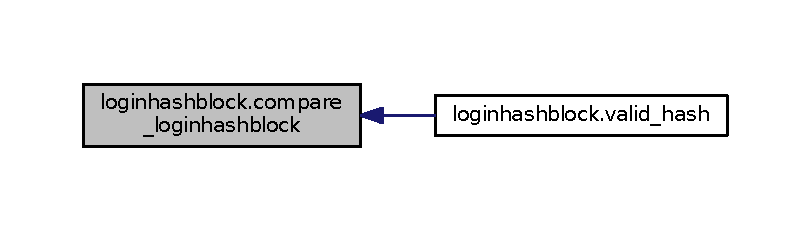
\includegraphics[width=350pt]{namespaceloginhashblock_ac24dd842eb90e0ede55e842d44148d5b_icgraph}
\end{center}
\end{figure}


\index{loginhashblock@{loginhashblock}!create\+\_\+device\+Id@{create\+\_\+device\+Id}}
\index{create\+\_\+device\+Id@{create\+\_\+device\+Id}!loginhashblock@{loginhashblock}}
\subsubsection[{\texorpdfstring{create\+\_\+device\+Id(\+D\+E\+B\+U\+G=\+False)}{create_deviceId(DEBUG=False)}}]{\setlength{\rightskip}{0pt plus 5cm}def loginhashblock.\+create\+\_\+device\+Id (
\begin{DoxyParamCaption}
\item[{}]{D\+E\+B\+UG = {\ttfamily False}}
\end{DoxyParamCaption}
)}\hypertarget{namespaceloginhashblock_a1bd31fe2f0ea4e6673127d72b6c42826}{}\label{namespaceloginhashblock_a1bd31fe2f0ea4e6673127d72b6c42826}
\begin{DoxyVerb}This function is to generate device Id
:return:
\end{DoxyVerb}
 

Definition at line 215 of file loginhashblock.\+py.


\begin{DoxyCode}
215 \textcolor{keyword}{def }\hyperlink{namespaceloginhashblock_a1bd31fe2f0ea4e6673127d72b6c42826}{create\_deviceId}(DEBUG=False):
216     \textcolor{stringliteral}{"""}
217 \textcolor{stringliteral}{    This function is to generate device Id}
218 \textcolor{stringliteral}{    :return:}
219 \textcolor{stringliteral}{    """}
220 
221     RAND\_CHARS = \textcolor{stringliteral}{"abcdefghijklmnopqrstuvwxyzABCDEFGHIJKLMNOPQRSTUVWXYZ0123456789"}
222     devid = \hyperlink{namespaceloginhashblock_afe116dea3aaff238a5fa2bcd6edf2281}{create\_salt}(8, RAND\_CHARS=RAND\_CHARS)
223 
224     \textcolor{keywordflow}{if} DEBUG:
225         text = \textcolor{stringliteral}{"[info:create\_deviceId] devid: \{\}"}.format(devid)
226         print(text)
227 
228     \textcolor{keywordflow}{return} devid
229 
\end{DoxyCode}


Here is the call graph for this function\+:
\nopagebreak
\begin{figure}[H]
\begin{center}
\leavevmode
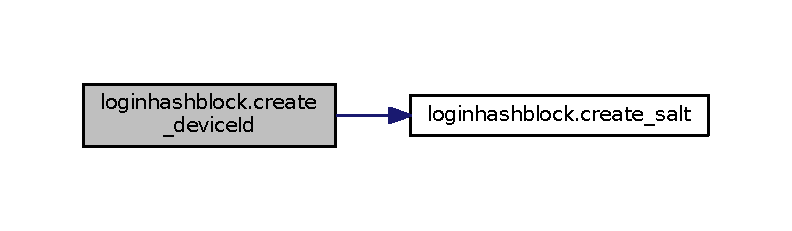
\includegraphics[width=350pt]{namespaceloginhashblock_a1bd31fe2f0ea4e6673127d72b6c42826_cgraph}
\end{center}
\end{figure}




Here is the caller graph for this function\+:
\nopagebreak
\begin{figure}[H]
\begin{center}
\leavevmode
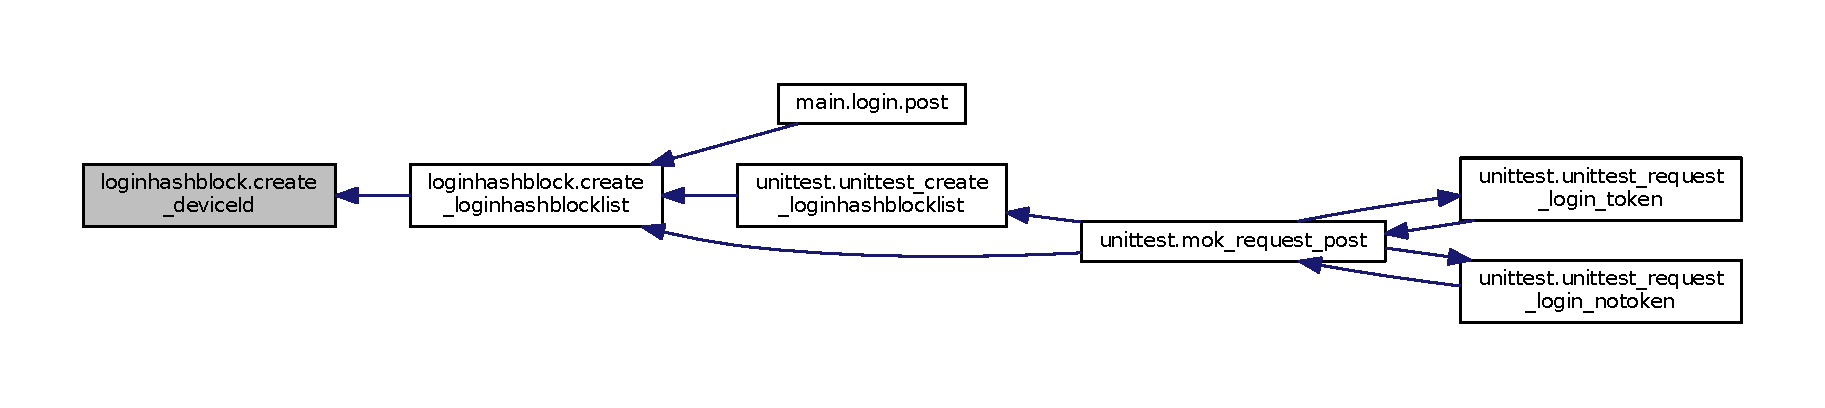
\includegraphics[width=350pt]{namespaceloginhashblock_a1bd31fe2f0ea4e6673127d72b6c42826_icgraph}
\end{center}
\end{figure}


\index{loginhashblock@{loginhashblock}!create\+\_\+hash@{create\+\_\+hash}}
\index{create\+\_\+hash@{create\+\_\+hash}!loginhashblock@{loginhashblock}}
\subsubsection[{\texorpdfstring{create\+\_\+hash(salt, target, hash\+\_\+name=""sha256"", iterations=100000, kdf=\+None, D\+E\+B\+U\+G=\+False)}{create_hash(salt, target, hash_name="sha256", iterations=100000, kdf=None, DEBUG=False)}}]{\setlength{\rightskip}{0pt plus 5cm}def loginhashblock.\+create\+\_\+hash (
\begin{DoxyParamCaption}
\item[{}]{salt, }
\item[{}]{target, }
\item[{}]{hash\+\_\+name = {\ttfamily \char`\"{}sha256\char`\"{}}, }
\item[{}]{iterations = {\ttfamily 100000}, }
\item[{}]{kdf = {\ttfamily None}, }
\item[{}]{D\+E\+B\+UG = {\ttfamily False}}
\end{DoxyParamCaption}
)}\hypertarget{namespaceloginhashblock_a935d8ae1c51e50f9e5db6a1d5f02b1b8}{}\label{namespaceloginhashblock_a935d8ae1c51e50f9e5db6a1d5f02b1b8}
\begin{DoxyVerb}This function is to obtain the digest of the byte target string, It uses HMAC as pseudorandom function.
:param salt, target: Target and salt are interpreted as buffers of bytes.
:param hash_name: The string hash_name is the desired name of the hash digest algorithm for HMAC
:param iterations: The number of iterations should be chosen based on the hash algorithm and computing power. As of 2013, at least 100,000 iterations of SHA-256 are suggested.
:param kdf: key derivation function(ex, bcrypt, PBKDF2 etc)
:return:
\end{DoxyVerb}
 

Definition at line 139 of file loginhashblock.\+py.


\begin{DoxyCode}
139 \textcolor{keyword}{def }\hyperlink{namespaceloginhashblock_a935d8ae1c51e50f9e5db6a1d5f02b1b8}{create\_hash}(salt, target, hash\_name="sha256", iterations=100000, kdf=None, DEBUG=False):
140     \textcolor{stringliteral}{"""}
141 \textcolor{stringliteral}{    This function is to obtain the digest of the byte target string, It uses HMAC as pseudorandom function.}
142 \textcolor{stringliteral}{    :param salt, target: Target and salt are interpreted as buffers of bytes.}
143 \textcolor{stringliteral}{    :param hash\_name: The string hash\_name is the desired name of the hash digest algorithm for HMAC}
144 \textcolor{stringliteral}{    :param iterations: The number of iterations should be chosen based on the hash algorithm and computing
       power. As of 2013, at least 100,000 iterations of SHA-256 are suggested.}
145 \textcolor{stringliteral}{    :param kdf: key derivation function(ex, bcrypt, PBKDF2 etc)}
146 \textcolor{stringliteral}{    :return:}
147 \textcolor{stringliteral}{    """}
148 
149     \textcolor{keywordflow}{if} \textcolor{keywordflow}{not} target \textcolor{keywordflow}{or} \textcolor{keywordflow}{not} salt:
150         \textcolor{keywordflow}{raise} ValueError(\textcolor{stringliteral}{"[info:create\_hash] target string or salt is null"})
151 
152     \textcolor{keywordflow}{if} \textcolor{keywordflow}{not} kdf:
153         h = hashlib.new(hash\_name)
154         h.update(target.encode(\textcolor{stringliteral}{'ascii'}))
155         hash = h.hexdigest()
156         method = \textcolor{stringliteral}{"none:%s:%d"} % (hash\_name, iterations)
157     \textcolor{keywordflow}{else}:
158         \textcolor{keywordflow}{if} kdf == \textcolor{stringliteral}{"pbkdf2"}:
159             hash = \hyperlink{namespaceloginhashblock_a104d0a92cdfb6c337794b6ded42667d4}{pbkdf2\_hash}(target, salt, iterations, hash\_name=hash\_name)
160             method = \textcolor{stringliteral}{"pbkdf2:%s:%d"} % (hash\_name, iterations)
161         \textcolor{keywordflow}{elif} kdf == \textcolor{stringliteral}{"scrypt"}:
162             \textcolor{keywordflow}{raise} ValueError(\textcolor{stringliteral}{"[info:create\_hash] will be supported"})
163         \textcolor{keywordflow}{else}:
164             \textcolor{keywordflow}{raise} ValueError(\textcolor{stringliteral}{"[info:create\_hash] Invalid support key derivation function"})
165 
166     \textcolor{keywordflow}{if} DEBUG:
167         text = \textcolor{stringliteral}{"[info:create\_hash] hash: \{\}, method: \{\}"}.format(hash, method)
168         print(text)
169 
170     \textcolor{keywordflow}{return} hash, method
171 
\end{DoxyCode}


Here is the call graph for this function\+:
\nopagebreak
\begin{figure}[H]
\begin{center}
\leavevmode
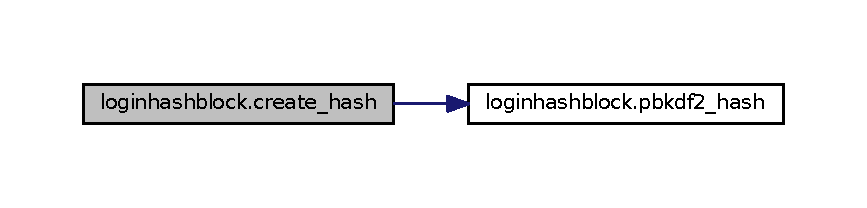
\includegraphics[width=350pt]{namespaceloginhashblock_a935d8ae1c51e50f9e5db6a1d5f02b1b8_cgraph}
\end{center}
\end{figure}




Here is the caller graph for this function\+:
\nopagebreak
\begin{figure}[H]
\begin{center}
\leavevmode
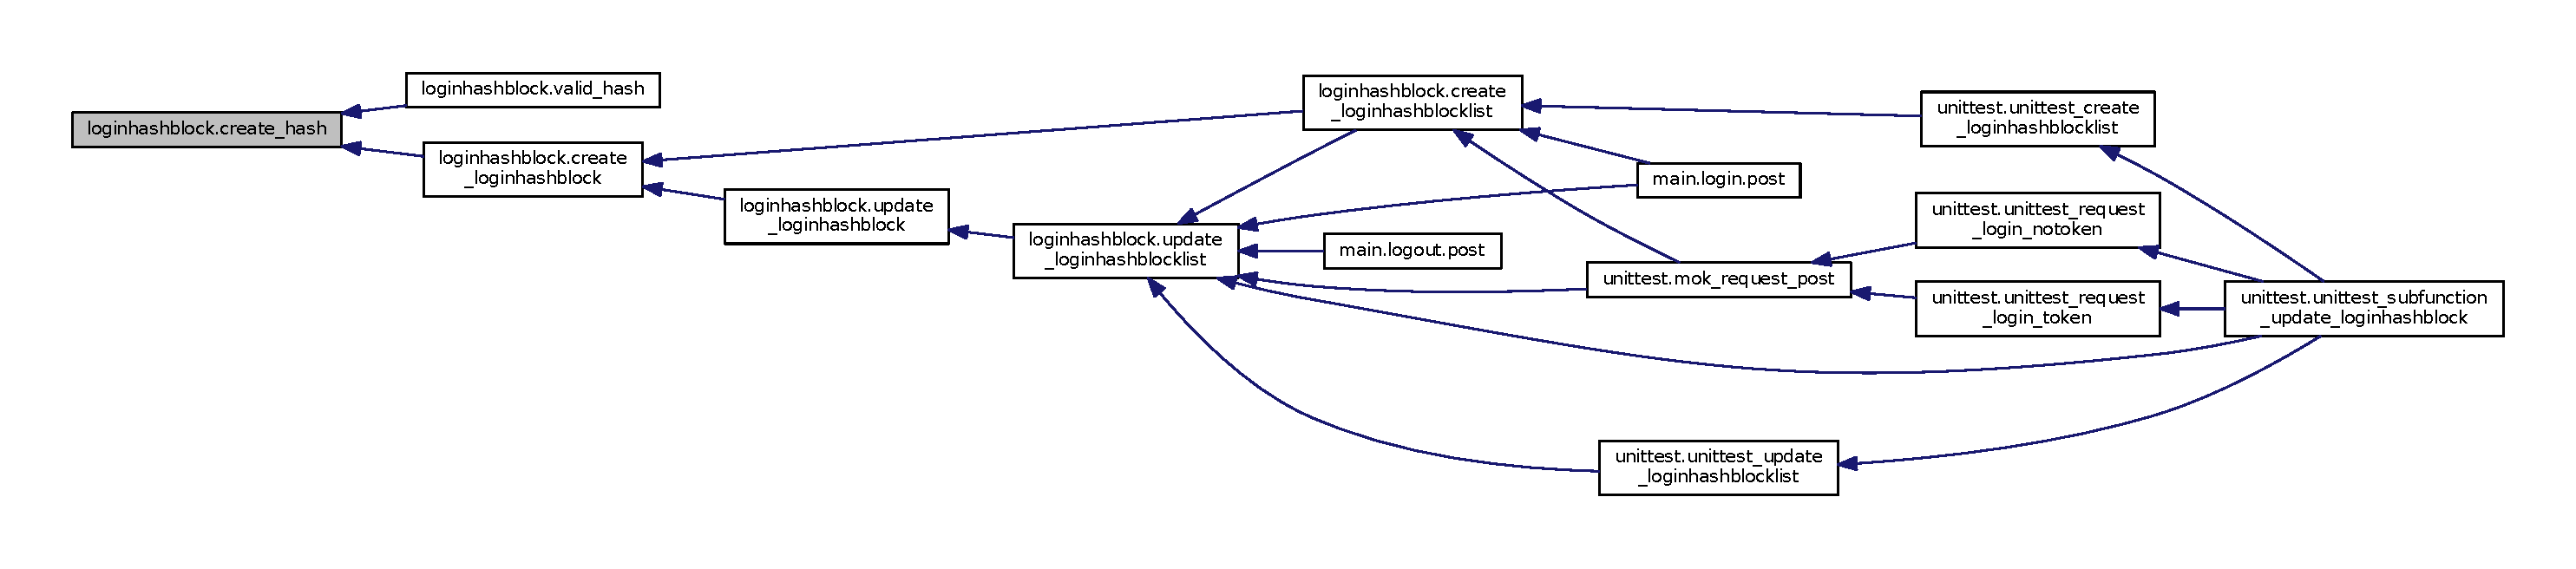
\includegraphics[width=350pt]{namespaceloginhashblock_a935d8ae1c51e50f9e5db6a1d5f02b1b8_icgraph}
\end{center}
\end{figure}


\index{loginhashblock@{loginhashblock}!create\+\_\+loginhashblock@{create\+\_\+loginhashblock}}
\index{create\+\_\+loginhashblock@{create\+\_\+loginhashblock}!loginhashblock@{loginhashblock}}
\subsubsection[{\texorpdfstring{create\+\_\+loginhashblock(devid, key=\+None, D\+E\+B\+U\+G=\+False)}{create_loginhashblock(devid, key=None, DEBUG=False)}}]{\setlength{\rightskip}{0pt plus 5cm}def loginhashblock.\+create\+\_\+loginhashblock (
\begin{DoxyParamCaption}
\item[{}]{devid, }
\item[{}]{key = {\ttfamily None}, }
\item[{}]{D\+E\+B\+UG = {\ttfamily False}}
\end{DoxyParamCaption}
)}\hypertarget{namespaceloginhashblock_ad3ef8dab740c69ca8424797f9c146a53}{}\label{namespaceloginhashblock_ad3ef8dab740c69ca8424797f9c146a53}
\begin{DoxyVerb}This functions is to generate login hash block with devid
:param devid:
:param key:
:return: login hash block
\end{DoxyVerb}
 

Definition at line 381 of file loginhashblock.\+py.


\begin{DoxyCode}
381 \textcolor{keyword}{def }\hyperlink{namespaceloginhashblock_ad3ef8dab740c69ca8424797f9c146a53}{create\_loginhashblock}(devid, key=None, DEBUG=False):
382     \textcolor{stringliteral}{"""}
383 \textcolor{stringliteral}{    This functions is to generate login hash block with devid}
384 \textcolor{stringliteral}{    :param devid:}
385 \textcolor{stringliteral}{    :param key:}
386 \textcolor{stringliteral}{    :return: login hash block}
387 \textcolor{stringliteral}{    """}
388 
389     \textcolor{keywordflow}{if} \textcolor{keywordflow}{not} devid:
390         \textcolor{keywordflow}{raise} ValueError(\textcolor{stringliteral}{"[info:create\_loginhashblock] devid is null"})
391 
392     \textcolor{keywordflow}{if} \textcolor{keywordflow}{not} key:
393         key = \textcolor{stringliteral}{'HKAHJFKIIJF'}
394 
395     length = 8
396     kdf = \textcolor{stringliteral}{'pbkdf2'}
397     salt = \hyperlink{namespaceloginhashblock_afe116dea3aaff238a5fa2bcd6edf2281}{create\_salt}(length)
398     hash, method = \hyperlink{namespaceloginhashblock_a935d8ae1c51e50f9e5db6a1d5f02b1b8}{create\_hash}(salt, key, kdf=kdf)
399 
400     \textcolor{keywordflow}{if} DEBUG:
401         text = \textcolor{stringliteral}{"[info:create\_loginhashblock] salt: \{\}, method: \{\}, hash: \{\}, devid: \{\}"}.format(salt, method
      , hash, devid)
402         print(text)
403 
404     LHBstr = \textcolor{stringliteral}{'\{\}$\{\}'}.format(devid, hash)
405 
406     \textcolor{keywordflow}{return} LHBstr
407 \end{DoxyCode}


Here is the call graph for this function\+:
\nopagebreak
\begin{figure}[H]
\begin{center}
\leavevmode
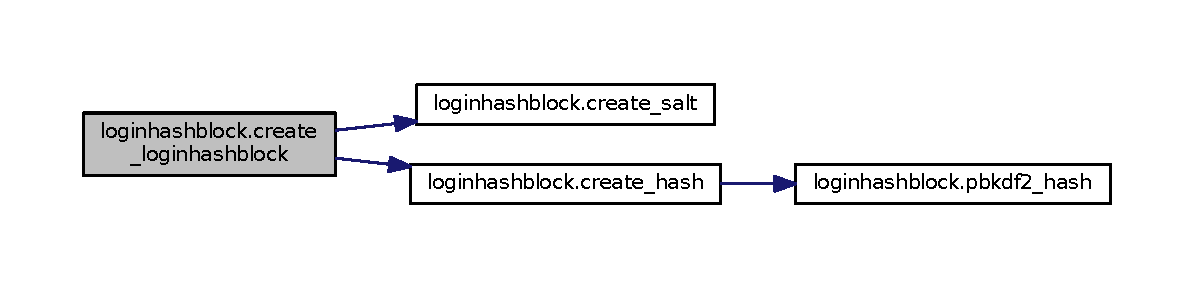
\includegraphics[width=350pt]{namespaceloginhashblock_ad3ef8dab740c69ca8424797f9c146a53_cgraph}
\end{center}
\end{figure}




Here is the caller graph for this function\+:
\nopagebreak
\begin{figure}[H]
\begin{center}
\leavevmode
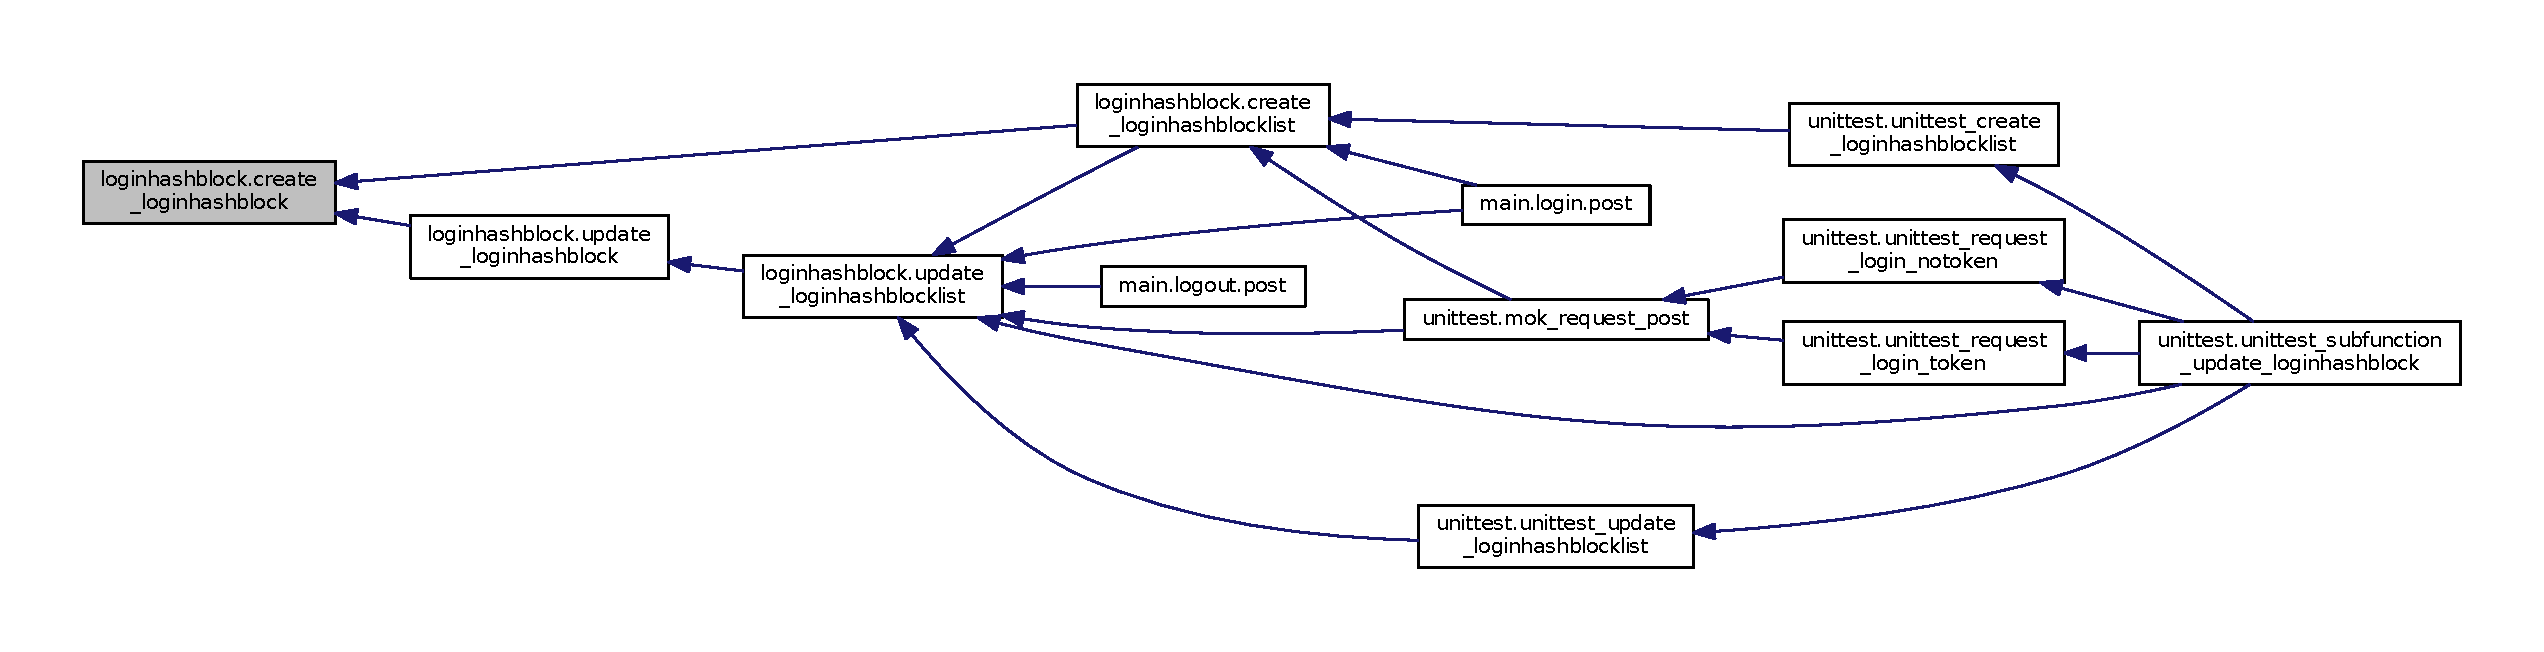
\includegraphics[width=350pt]{namespaceloginhashblock_ad3ef8dab740c69ca8424797f9c146a53_icgraph}
\end{center}
\end{figure}


\index{loginhashblock@{loginhashblock}!create\+\_\+loginhashblocklist@{create\+\_\+loginhashblocklist}}
\index{create\+\_\+loginhashblocklist@{create\+\_\+loginhashblocklist}!loginhashblock@{loginhashblock}}
\subsubsection[{\texorpdfstring{create\+\_\+loginhashblocklist(\+L\+H\+Blist\+Str, D\+E\+B\+U\+G=\+D\+E\+B\+U\+G)}{create_loginhashblocklist(LHBlistStr, DEBUG=DEBUG)}}]{\setlength{\rightskip}{0pt plus 5cm}def loginhashblock.\+create\+\_\+loginhashblocklist (
\begin{DoxyParamCaption}
\item[{}]{L\+H\+Blist\+Str, }
\item[{}]{D\+E\+B\+UG = {\ttfamily {\bf D\+E\+B\+UG}}}
\end{DoxyParamCaption}
)}\hypertarget{namespaceloginhashblock_a550707107141dfb228ca4294d7ea31b4}{}\label{namespaceloginhashblock_a550707107141dfb228ca4294d7ea31b4}
\begin{DoxyVerb}This function generate login hash block list
:param LHBlistStr: previous login hash block list
:return:
\end{DoxyVerb}
 

Definition at line 84 of file loginhashblock.\+py.


\begin{DoxyCode}
84 \textcolor{keyword}{def }\hyperlink{namespaceloginhashblock_a550707107141dfb228ca4294d7ea31b4}{create\_loginhashblocklist}(LHBlistStr, DEBUG=DEBUG):
85     \textcolor{stringliteral}{"""}
86 \textcolor{stringliteral}{    This function generate login hash block list}
87 \textcolor{stringliteral}{    :param LHBlistStr: previous login hash block list}
88 \textcolor{stringliteral}{    :return:}
89 \textcolor{stringliteral}{    """}
90 
91     devid = \hyperlink{namespaceloginhashblock_a1bd31fe2f0ea4e6673127d72b6c42826}{create\_deviceId}(DEBUG=DEBUG)
92     LHBstr = \hyperlink{namespaceloginhashblock_ad3ef8dab740c69ca8424797f9c146a53}{create\_loginhashblock}(devid, DEBUG=DEBUG)
93     uLHBlistStr, uLHBstr = \hyperlink{namespaceloginhashblock_a2bcc7ddd0fcc3788572dd77808cb624d}{update\_loginhashblocklist}(LHBlistStr, LHBstr)
94 
95     \textcolor{keywordflow}{return} uLHBlistStr, uLHBstr
96 
\end{DoxyCode}


Here is the call graph for this function\+:
\nopagebreak
\begin{figure}[H]
\begin{center}
\leavevmode
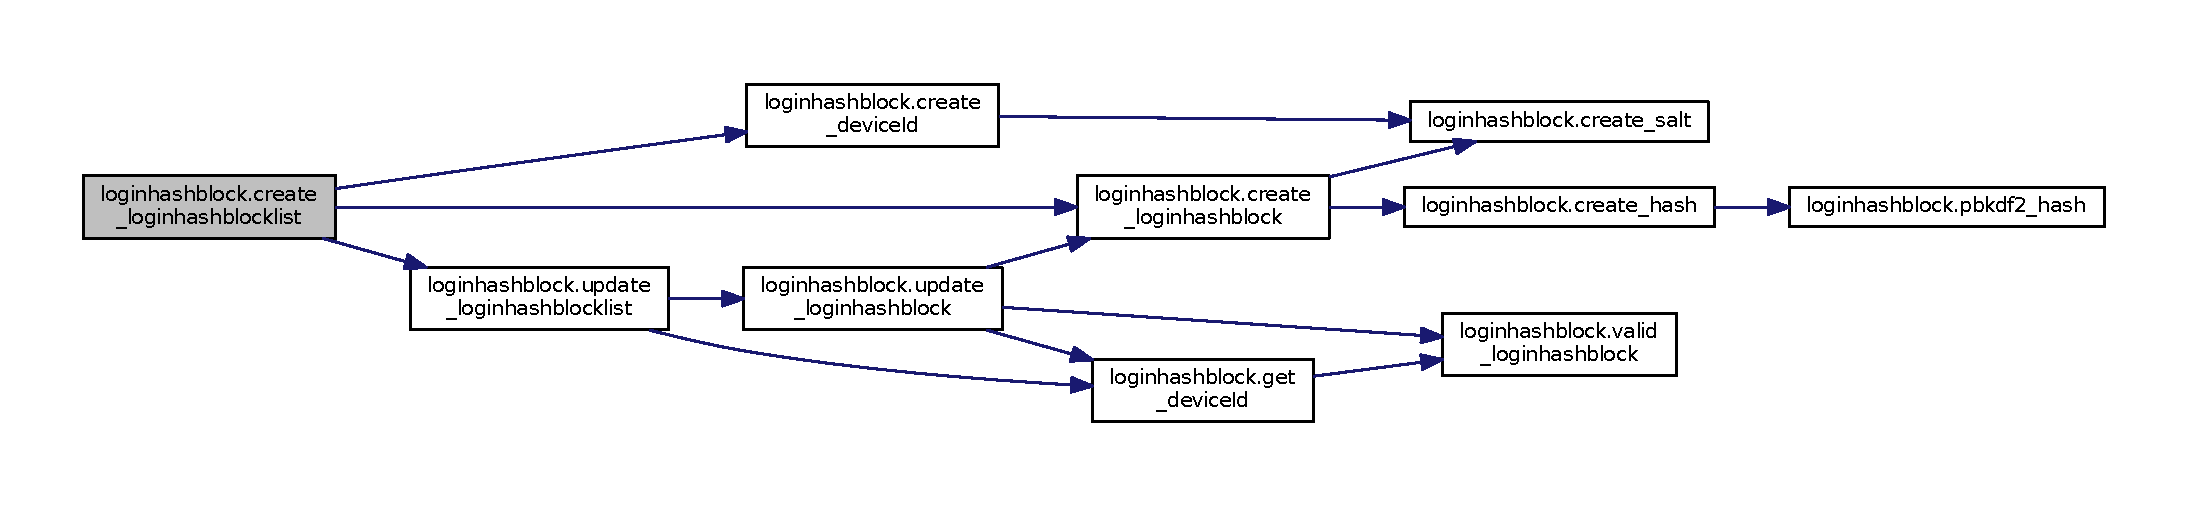
\includegraphics[width=350pt]{namespaceloginhashblock_a550707107141dfb228ca4294d7ea31b4_cgraph}
\end{center}
\end{figure}




Here is the caller graph for this function\+:
\nopagebreak
\begin{figure}[H]
\begin{center}
\leavevmode
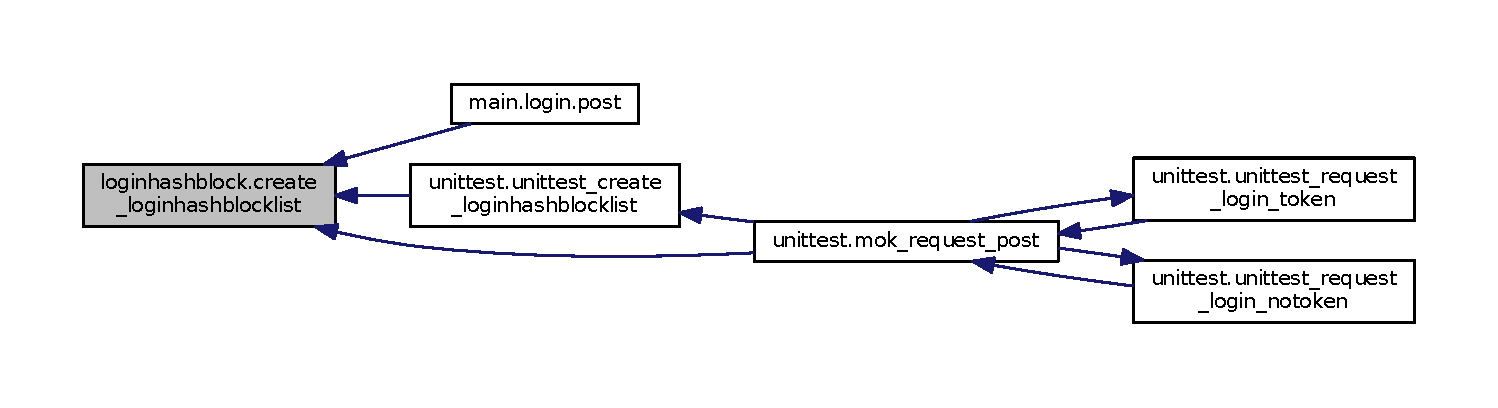
\includegraphics[width=350pt]{namespaceloginhashblock_a550707107141dfb228ca4294d7ea31b4_icgraph}
\end{center}
\end{figure}


\index{loginhashblock@{loginhashblock}!create\+\_\+salt@{create\+\_\+salt}}
\index{create\+\_\+salt@{create\+\_\+salt}!loginhashblock@{loginhashblock}}
\subsubsection[{\texorpdfstring{create\+\_\+salt(length, R\+A\+N\+D\+\_\+\+C\+H\+A\+R\+S=\+None, D\+E\+B\+U\+G=\+False)}{create_salt(length, RAND_CHARS=None, DEBUG=False)}}]{\setlength{\rightskip}{0pt plus 5cm}def loginhashblock.\+create\+\_\+salt (
\begin{DoxyParamCaption}
\item[{}]{length, }
\item[{}]{R\+A\+N\+D\+\_\+\+C\+H\+A\+RS = {\ttfamily None}, }
\item[{}]{D\+E\+B\+UG = {\ttfamily False}}
\end{DoxyParamCaption}
)}\hypertarget{namespaceloginhashblock_afe116dea3aaff238a5fa2bcd6edf2281}{}\label{namespaceloginhashblock_afe116dea3aaff238a5fa2bcd6edf2281}
\begin{DoxyVerb}This function generate a random string of SALT_CHARS with specified length.
:param length: salt length
:param RAND_CHARS: random chars
:return:
\end{DoxyVerb}
 

Definition at line 67 of file loginhashblock.\+py.


\begin{DoxyCode}
67 \textcolor{keyword}{def }\hyperlink{namespaceloginhashblock_afe116dea3aaff238a5fa2bcd6edf2281}{create\_salt}(length, RAND\_CHARS=None, DEBUG=False):
68     \textcolor{stringliteral}{"""}
69 \textcolor{stringliteral}{    This function generate a random string of SALT\_CHARS with specified length.}
70 \textcolor{stringliteral}{    :param length: salt length}
71 \textcolor{stringliteral}{    :param RAND\_CHARS: random chars}
72 \textcolor{stringliteral}{    :return:}
73 \textcolor{stringliteral}{    """}
74     \textcolor{keywordflow}{if} \textcolor{keywordflow}{not} RAND\_CHARS:
75         RAND\_CHARS = \textcolor{stringliteral}{"abcdefghijklmnopqrstuvwxyzABCDEFGHIJKLMNOPQRSTUVWXYZ0123456789!@#%^&*()"}
76 
77     randx = list()
78     \textcolor{keywordflow}{for} x \textcolor{keywordflow}{in} range(length):
79          randx.append(random.choice(RAND\_CHARS))
80 
81     salt = \textcolor{stringliteral}{''}.join(randx)
82     \textcolor{keywordflow}{return} salt
83 
\end{DoxyCode}


Here is the caller graph for this function\+:
\nopagebreak
\begin{figure}[H]
\begin{center}
\leavevmode
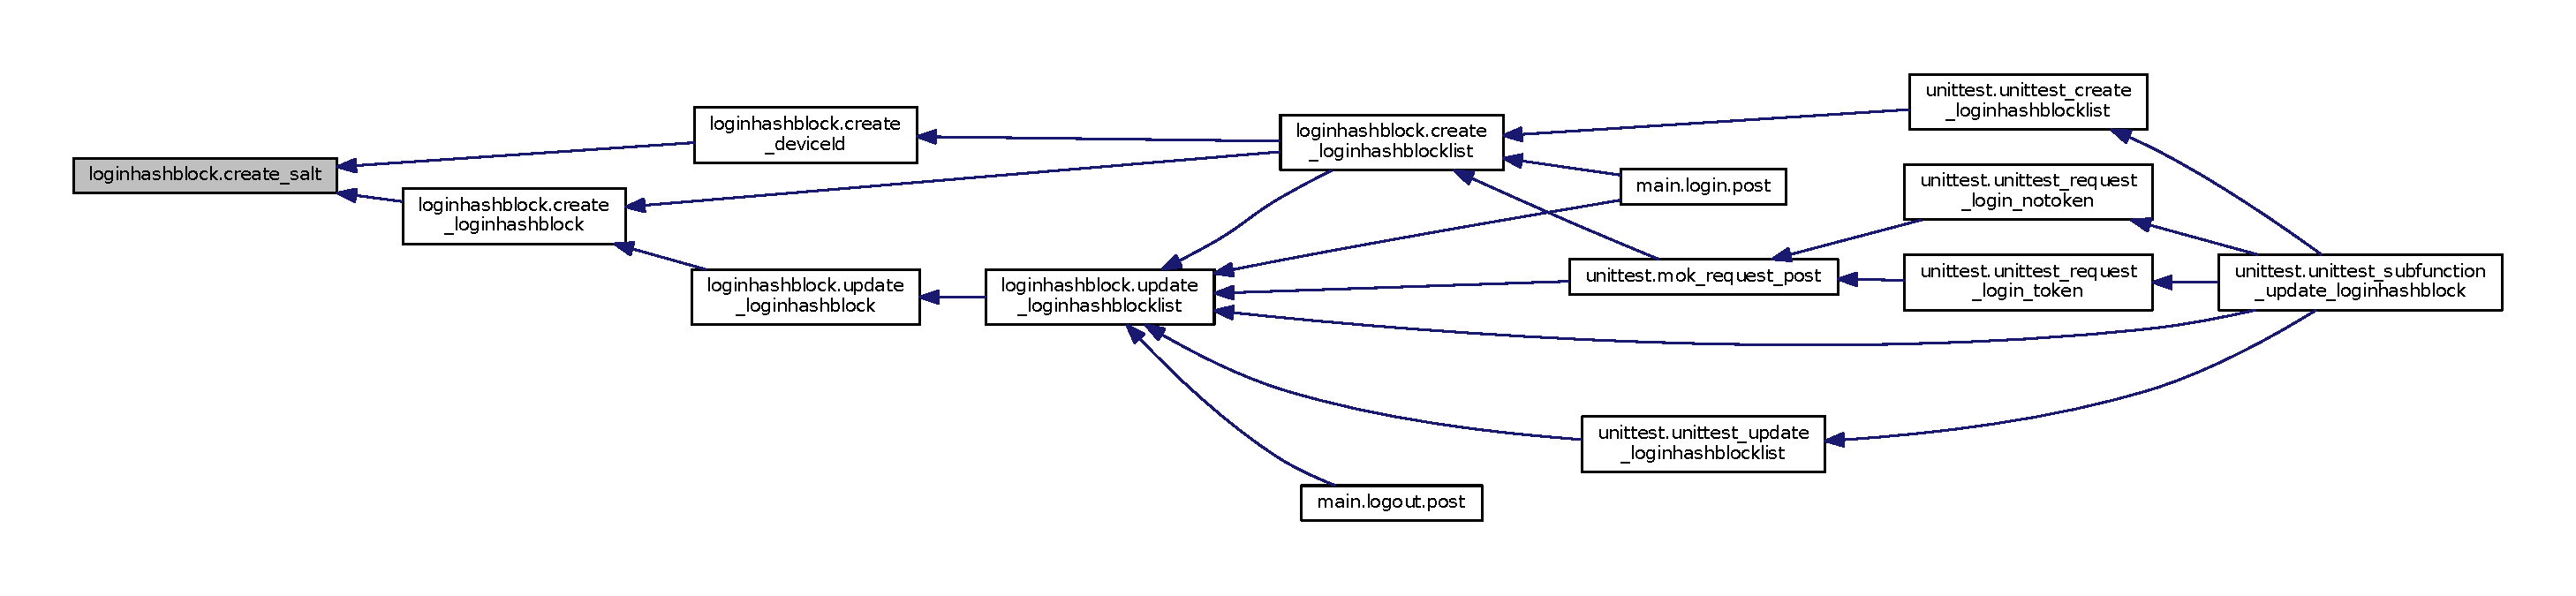
\includegraphics[width=350pt]{namespaceloginhashblock_afe116dea3aaff238a5fa2bcd6edf2281_icgraph}
\end{center}
\end{figure}


\index{loginhashblock@{loginhashblock}!get\+\_\+device\+Id@{get\+\_\+device\+Id}}
\index{get\+\_\+device\+Id@{get\+\_\+device\+Id}!loginhashblock@{loginhashblock}}
\subsubsection[{\texorpdfstring{get\+\_\+device\+Id(\+L\+H\+Bstr, D\+E\+B\+U\+G=\+False)}{get_deviceId(LHBstr, DEBUG=False)}}]{\setlength{\rightskip}{0pt plus 5cm}def loginhashblock.\+get\+\_\+device\+Id (
\begin{DoxyParamCaption}
\item[{}]{L\+H\+Bstr, }
\item[{}]{D\+E\+B\+UG = {\ttfamily False}}
\end{DoxyParamCaption}
)}\hypertarget{namespaceloginhashblock_a17417f2f6bca76ab51170082a562e5f6}{}\label{namespaceloginhashblock_a17417f2f6bca76ab51170082a562e5f6}
\begin{DoxyVerb}This function is to get device id from login hash block
:param LHBstr:
:return:
\end{DoxyVerb}
 

Definition at line 196 of file loginhashblock.\+py.


\begin{DoxyCode}
196 \textcolor{keyword}{def }\hyperlink{namespaceloginhashblock_a17417f2f6bca76ab51170082a562e5f6}{get\_deviceId}(LHBstr, DEBUG=False):
197     \textcolor{stringliteral}{"""}
198 \textcolor{stringliteral}{    This function is to get device id from login hash block}
199 \textcolor{stringliteral}{    :param LHBstr:}
200 \textcolor{stringliteral}{    :return:}
201 \textcolor{stringliteral}{    """}
202 
203     \textcolor{keywordflow}{if} DEBUG:
204         print(\textcolor{stringliteral}{"[info:get\_deviceId] LHBstr: \{\}"}.format(LHBstr))
205 
206     \textcolor{keywordflow}{if} \textcolor{keywordflow}{not} LHBstr:
207         \textcolor{keywordflow}{raise} ValueError(\textcolor{stringliteral}{"[info:get\_deviceId] login hash block is null"})
208 
209     \textcolor{keywordflow}{if} \textcolor{keywordflow}{not} \hyperlink{namespaceloginhashblock_adb424539d851426da7b65d53c5a6d577}{valid\_loginhashblock}(LHBstr, DEBUG=DEBUG):
210         \textcolor{keywordflow}{raise} ValueError(\textcolor{stringliteral}{"[info:get\_deviceId] Invalid login hash block"})
211 
212     devid, loginhash = LHBstr.split(\textcolor{stringliteral}{"$"}, 1)
213     \textcolor{keywordflow}{return} devid
214 
\end{DoxyCode}


Here is the call graph for this function\+:
\nopagebreak
\begin{figure}[H]
\begin{center}
\leavevmode
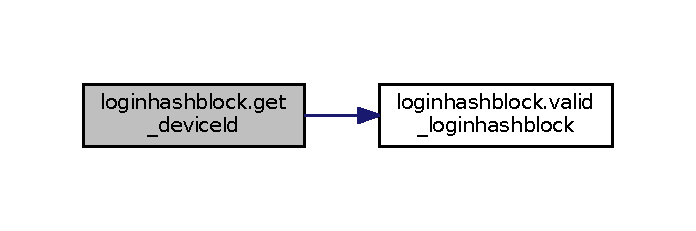
\includegraphics[width=334pt]{namespaceloginhashblock_a17417f2f6bca76ab51170082a562e5f6_cgraph}
\end{center}
\end{figure}




Here is the caller graph for this function\+:
\nopagebreak
\begin{figure}[H]
\begin{center}
\leavevmode
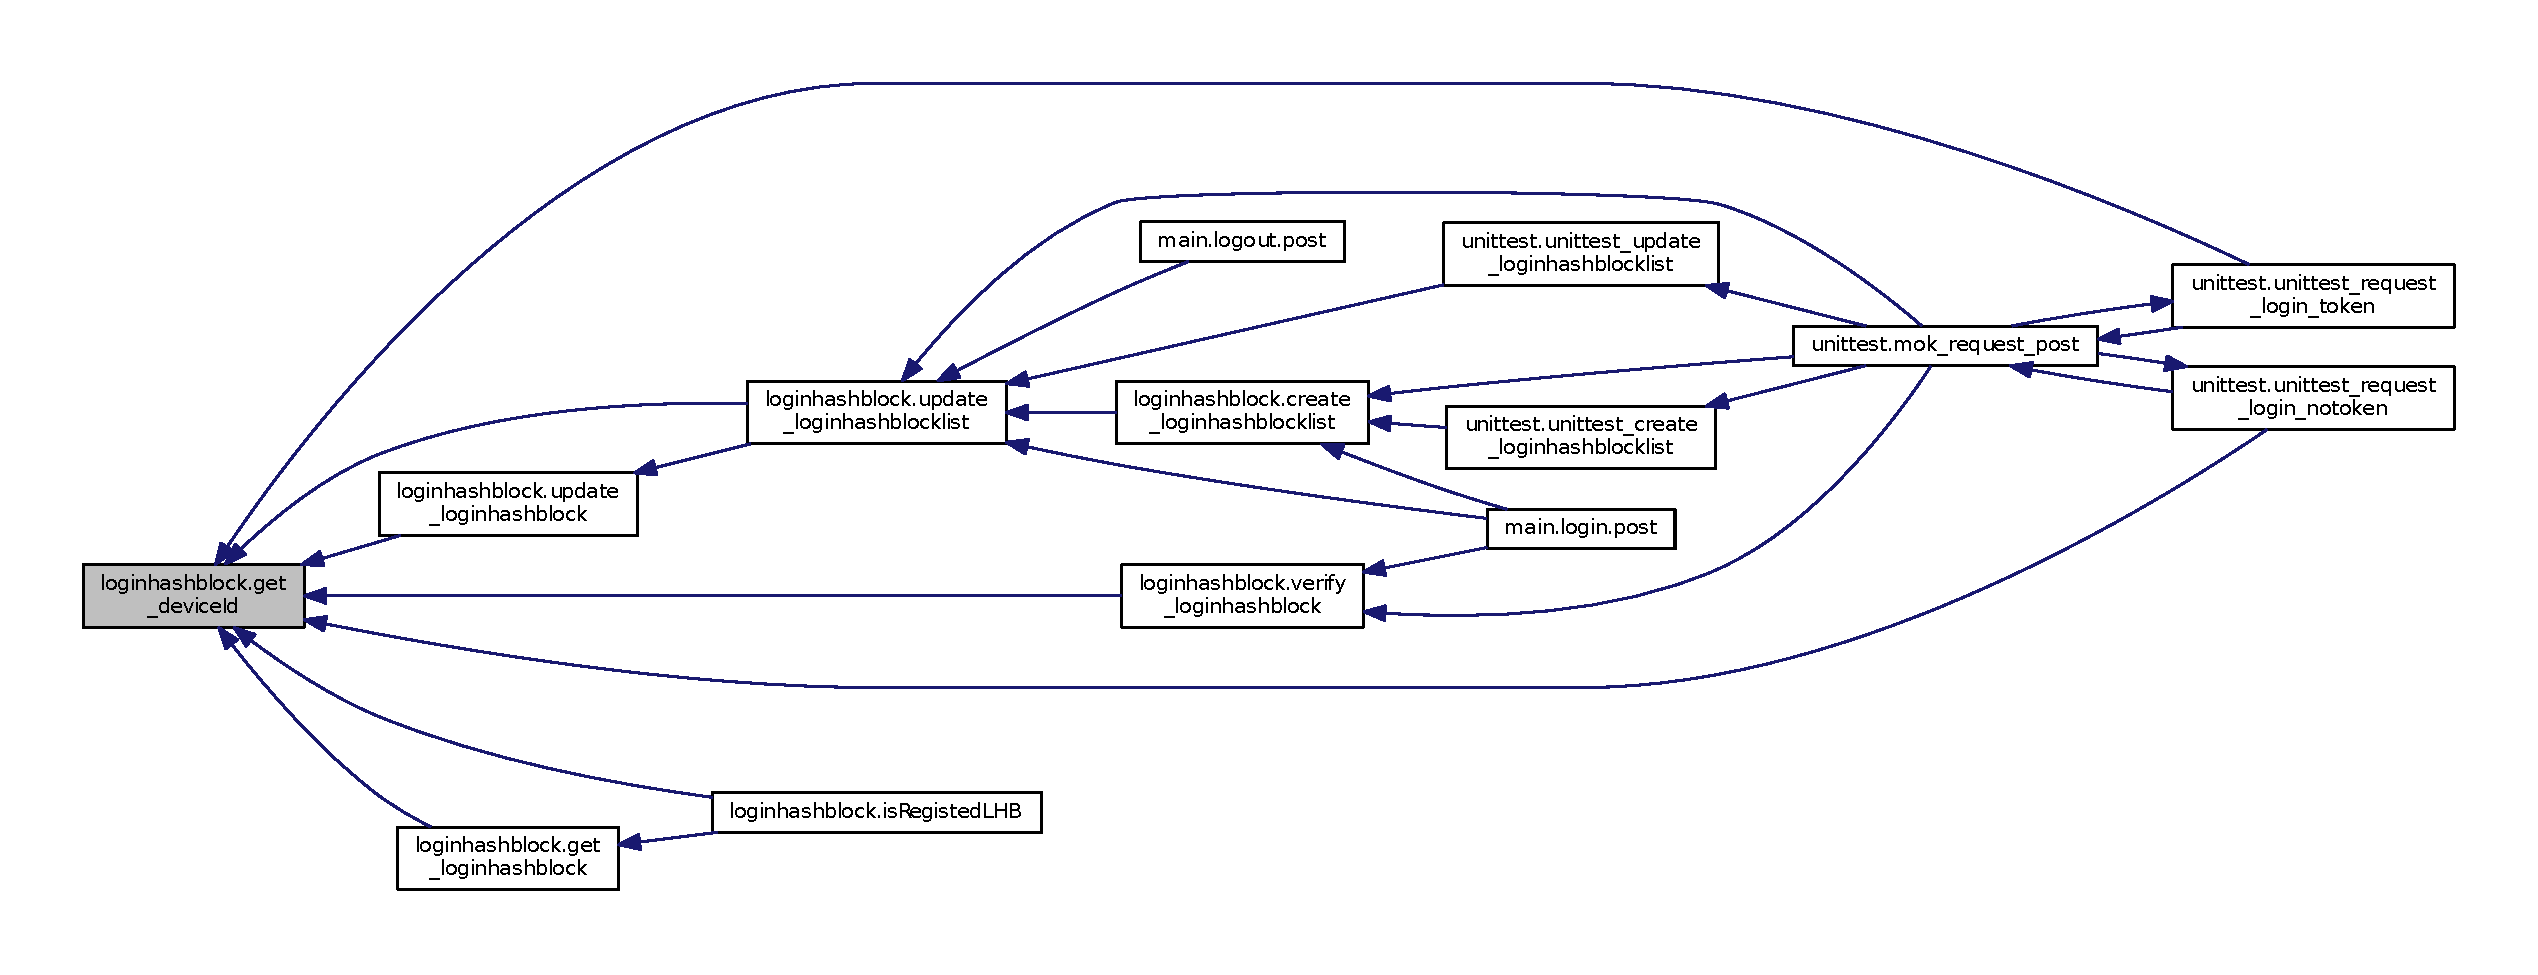
\includegraphics[width=350pt]{namespaceloginhashblock_a17417f2f6bca76ab51170082a562e5f6_icgraph}
\end{center}
\end{figure}


\index{loginhashblock@{loginhashblock}!get\+\_\+loginhashblock@{get\+\_\+loginhashblock}}
\index{get\+\_\+loginhashblock@{get\+\_\+loginhashblock}!loginhashblock@{loginhashblock}}
\subsubsection[{\texorpdfstring{get\+\_\+loginhashblock(devid, L\+H\+Blist, D\+E\+B\+U\+G=\+False)}{get_loginhashblock(devid, LHBlist, DEBUG=False)}}]{\setlength{\rightskip}{0pt plus 5cm}def loginhashblock.\+get\+\_\+loginhashblock (
\begin{DoxyParamCaption}
\item[{}]{devid, }
\item[{}]{L\+H\+Blist, }
\item[{}]{D\+E\+B\+UG = {\ttfamily False}}
\end{DoxyParamCaption}
)}\hypertarget{namespaceloginhashblock_a6187961cb9009c7836e7e6e639085f93}{}\label{namespaceloginhashblock_a6187961cb9009c7836e7e6e639085f93}
\begin{DoxyVerb}This function is to get login hash block by device id in login hash block list.
:devid: device id
:LHBlist: client's login has block in database
:return:
\end{DoxyVerb}
 

Definition at line 361 of file loginhashblock.\+py.


\begin{DoxyCode}
361 \textcolor{keyword}{def }\hyperlink{namespaceloginhashblock_a6187961cb9009c7836e7e6e639085f93}{get\_loginhashblock}(devid, LHBlist, DEBUG=False):
362     \textcolor{stringliteral}{"""}
363 \textcolor{stringliteral}{    This function is to get login hash block by device id in login hash block list.}
364 \textcolor{stringliteral}{    :devid: device id}
365 \textcolor{stringliteral}{    :LHBlist: client's login has block in database}
366 \textcolor{stringliteral}{    :return:}
367 \textcolor{stringliteral}{    """}
368 
369     \textcolor{keywordflow}{for} LHBstr \textcolor{keywordflow}{in} LHBlist:
370         \_devid = \hyperlink{namespaceloginhashblock_a17417f2f6bca76ab51170082a562e5f6}{get\_deviceId}(LHBstr, DEBUG=DEBUG)
371         \textcolor{keywordflow}{if} devid == \_devid:
372             \textcolor{keywordflow}{if} DEBUG:
373                 print(\textcolor{stringliteral}{'[info:get\_loginhashblock] devid is found in login hash block list'})
374             \textcolor{keywordflow}{return} LHBstr
375 
376     \textcolor{keywordflow}{if} DEBUG:
377         print(\textcolor{stringliteral}{'[info:get\_loginhashblock] devid is not found in login hash block list'})
378 
379     \textcolor{keywordflow}{return} \textcolor{stringliteral}{''}
380 
\end{DoxyCode}


Here is the call graph for this function\+:
\nopagebreak
\begin{figure}[H]
\begin{center}
\leavevmode
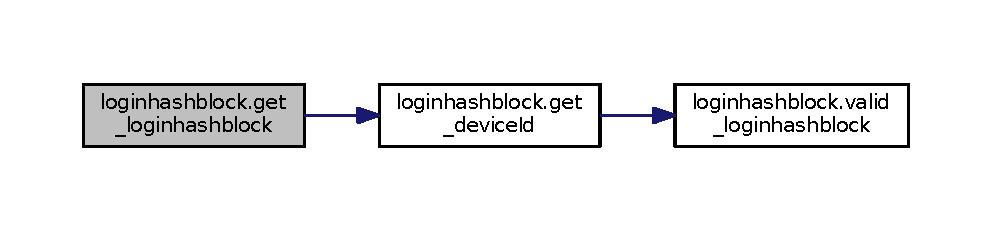
\includegraphics[width=350pt]{namespaceloginhashblock_a6187961cb9009c7836e7e6e639085f93_cgraph}
\end{center}
\end{figure}




Here is the caller graph for this function\+:
\nopagebreak
\begin{figure}[H]
\begin{center}
\leavevmode
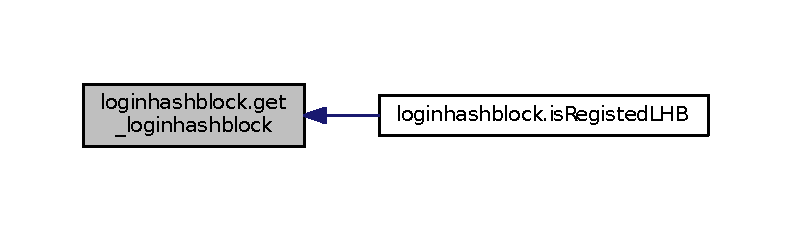
\includegraphics[width=350pt]{namespaceloginhashblock_a6187961cb9009c7836e7e6e639085f93_icgraph}
\end{center}
\end{figure}


\index{loginhashblock@{loginhashblock}!is\+Registed\+L\+HB@{is\+Registed\+L\+HB}}
\index{is\+Registed\+L\+HB@{is\+Registed\+L\+HB}!loginhashblock@{loginhashblock}}
\subsubsection[{\texorpdfstring{is\+Registed\+L\+H\+B(\+L\+H\+Bstr, L\+H\+Blist\+Str, D\+E\+B\+U\+G=\+False)}{isRegistedLHB(LHBstr, LHBlistStr, DEBUG=False)}}]{\setlength{\rightskip}{0pt plus 5cm}def loginhashblock.\+is\+Registed\+L\+HB (
\begin{DoxyParamCaption}
\item[{}]{L\+H\+Bstr, }
\item[{}]{L\+H\+Blist\+Str, }
\item[{}]{D\+E\+B\+UG = {\ttfamily False}}
\end{DoxyParamCaption}
)}\hypertarget{namespaceloginhashblock_a746d5c48cd93a76b78c90c34419ebdaa}{}\label{namespaceloginhashblock_a746d5c48cd93a76b78c90c34419ebdaa}
\begin{DoxyVerb}This function is to check valid previous login hash block.
:LHBstr: client's login hash block
:LHBlistStr: client's login has block in database
\end{DoxyVerb}
 

Definition at line 338 of file loginhashblock.\+py.


\begin{DoxyCode}
338 \textcolor{keyword}{def }\hyperlink{namespaceloginhashblock_a746d5c48cd93a76b78c90c34419ebdaa}{isRegistedLHB}(LHBstr, LHBlistStr, DEBUG=False):
339     \textcolor{stringliteral}{"""}
340 \textcolor{stringliteral}{    This function is to check valid previous login hash block.}
341 \textcolor{stringliteral}{    :LHBstr: client's login hash block}
342 \textcolor{stringliteral}{    :LHBlistStr: client's login has block in database}
343 \textcolor{stringliteral}{    """}
344 
345     LHBlist = LHBlistStr.split(\textcolor{stringliteral}{','})
346 
347     \textcolor{keywordflow}{if} \textcolor{keywordflow}{not} \hyperlink{namespaceloginhashblock_adb424539d851426da7b65d53c5a6d577}{valid\_loginhashblock}(LHBstr, DEBUG=DEBUG):
348         \textcolor{keywordflow}{return} \textcolor{keyword}{False}
349 
350     devid = \hyperlink{namespaceloginhashblock_a17417f2f6bca76ab51170082a562e5f6}{get\_deviceId}(LHBstr, DEBUG=DEBUG)
351     target\_LHBstr = \hyperlink{namespaceloginhashblock_a6187961cb9009c7836e7e6e639085f93}{get\_loginhashblock}(devid, LHBlist, DEBUG=DEBUG)
352 
353     \textcolor{keywordflow}{if} DEBUG:
354         print(\textcolor{stringliteral}{"[info:isRegistedLHB]\(\backslash\)nclient\_loginhashblock: \{\}\(\backslash\)nserver\_loginhashblock: \{\}"}.format(LHBstr, 
      target\_LHBstr))
355 
356     \textcolor{keywordflow}{if} LHBstr == target\_LHBstr:
357         \textcolor{keywordflow}{return} \textcolor{keyword}{True}
358 
359     \textcolor{keywordflow}{return} \textcolor{keyword}{False}
360 
\end{DoxyCode}


Here is the call graph for this function\+:
\nopagebreak
\begin{figure}[H]
\begin{center}
\leavevmode
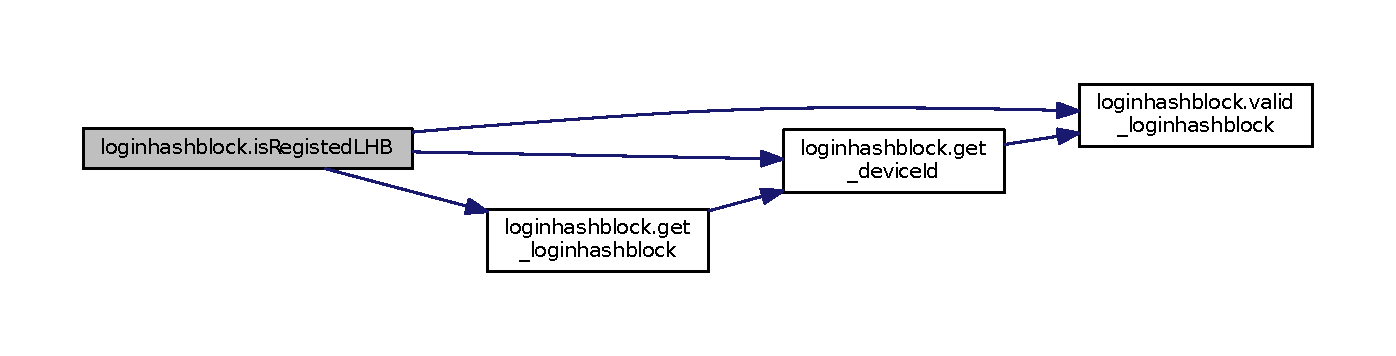
\includegraphics[width=350pt]{namespaceloginhashblock_a746d5c48cd93a76b78c90c34419ebdaa_cgraph}
\end{center}
\end{figure}


\index{loginhashblock@{loginhashblock}!pbkdf2\+\_\+hash@{pbkdf2\+\_\+hash}}
\index{pbkdf2\+\_\+hash@{pbkdf2\+\_\+hash}!loginhashblock@{loginhashblock}}
\subsubsection[{\texorpdfstring{pbkdf2\+\_\+hash(data, salt, iterations, dklen=\+None, hash\+\_\+name=""sha256"", D\+E\+B\+U\+G=\+False)}{pbkdf2_hash(data, salt, iterations, dklen=None, hash_name="sha256", DEBUG=False)}}]{\setlength{\rightskip}{0pt plus 5cm}def loginhashblock.\+pbkdf2\+\_\+hash (
\begin{DoxyParamCaption}
\item[{}]{data, }
\item[{}]{salt, }
\item[{}]{iterations, }
\item[{}]{dklen = {\ttfamily None}, }
\item[{}]{hash\+\_\+name = {\ttfamily \char`\"{}sha256\char`\"{}}, }
\item[{}]{D\+E\+B\+UG = {\ttfamily False}}
\end{DoxyParamCaption}
)}\hypertarget{namespaceloginhashblock_a104d0a92cdfb6c337794b6ded42667d4}{}\label{namespaceloginhashblock_a104d0a92cdfb6c337794b6ded42667d4}
\begin{DoxyVerb}The function provides PKCS#5 password-based key derivation function.
It uses HMAC as pseudorandom function.
eturn the hexadecimal representation of the binary data. Every byte of data is converted into the corresponding 2-digit hex representation.
:param data: data and salt are interpreted as buffers of byte
:param salt: data and salt are interpreted as buffers of byte
:param iterations: The number of iterations should be chosen based on the hash algorithm and computing power. As of 2013, at least 100,000 iterations of SHA-256 are suggested.
:param dklen: dklen is the length of the derived key. If dklen is None then the digest size of the hash algorithm hash_name is used, e.g. 64 for SHA-512.
:param hash_name: hash_name is the desired name of the hash digest algorithm for HMAC(default: sha256)
:return:
\end{DoxyVerb}
 

Definition at line 44 of file loginhashblock.\+py.


\begin{DoxyCode}
44 \textcolor{keyword}{def }\hyperlink{namespaceloginhashblock_a104d0a92cdfb6c337794b6ded42667d4}{pbkdf2\_hash}(data, salt, iterations, dklen=None, hash\_name="sha256", DEBUG=False):
45     \textcolor{stringliteral}{"""}
46 \textcolor{stringliteral}{    The function provides PKCS#5 password-based key derivation function.}
47 \textcolor{stringliteral}{    It uses HMAC as pseudorandom function.}
48 \textcolor{stringliteral}{    eturn the hexadecimal representation of the binary data. Every byte of data is converted into the
       corresponding 2-digit hex representation.}
49 \textcolor{stringliteral}{    :param data: data and salt are interpreted as buffers of byte}
50 \textcolor{stringliteral}{    :param salt: data and salt are interpreted as buffers of byte}
51 \textcolor{stringliteral}{    :param iterations: The number of iterations should be chosen based on the hash algorithm and computing
       power. As of 2013, at least 100,000 iterations of SHA-256 are suggested.}
52 \textcolor{stringliteral}{    :param dklen: dklen is the length of the derived key. If dklen is None then the digest size of the hash
       algorithm hash\_name is used, e.g. 64 for SHA-512.}
53 \textcolor{stringliteral}{    :param hash\_name: hash\_name is the desired name of the hash digest algorithm for HMAC(default: sha256)}
54 \textcolor{stringliteral}{    :return:}
55 \textcolor{stringliteral}{    """}
56 
57     \textcolor{keywordflow}{if} DEBUG:
58         print(\textcolor{stringliteral}{'[info:pdkdf2\_ascii] hash: '}, hash\_name)
59         print(\textcolor{stringliteral}{'[info:pdkdf2\_ascii] iterations: '}, iterations)
60         print(\textcolor{stringliteral}{'[info:pdkdf2\_ascii] data: '}, data.encode(\textcolor{stringliteral}{'ascii'}))
61         print(\textcolor{stringliteral}{'[info:pdkdf2\_ascii] salt: '}, salt.encode(\textcolor{stringliteral}{'ascii'}))
62 
63     dk = hashlib.pbkdf2\_hmac(hash\_name, data.encode(\textcolor{stringliteral}{'ascii'}), salt.encode(\textcolor{stringliteral}{'ascii'}), iterations, dklen=dklen
      )
64     hex = binascii.hexlify(dk)
65     \textcolor{keywordflow}{return} hex.decode(\textcolor{stringliteral}{'ascii'})
66 
\end{DoxyCode}


Here is the caller graph for this function\+:
\nopagebreak
\begin{figure}[H]
\begin{center}
\leavevmode
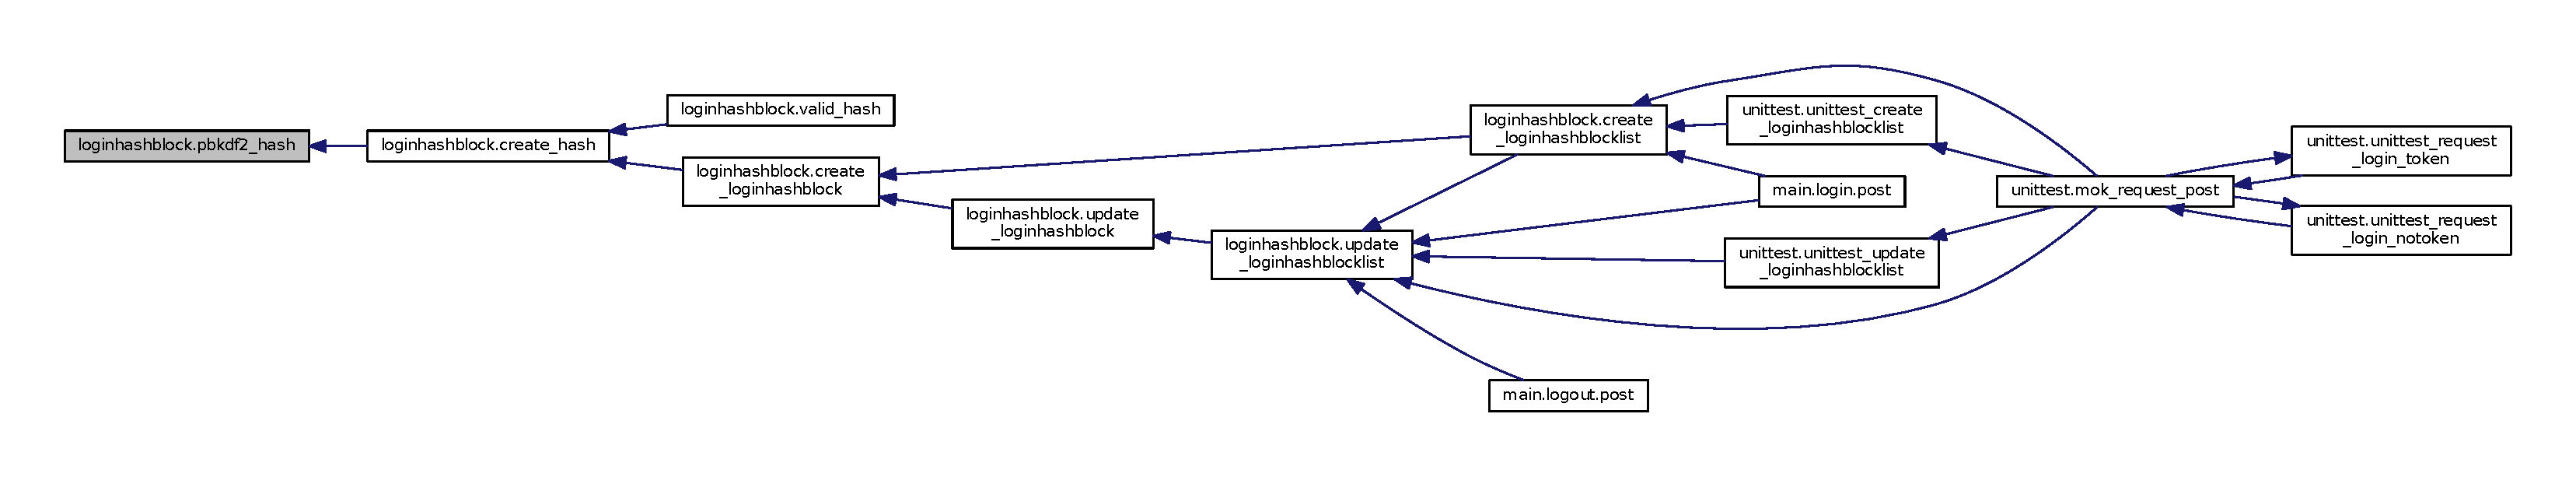
\includegraphics[width=350pt]{namespaceloginhashblock_a104d0a92cdfb6c337794b6ded42667d4_icgraph}
\end{center}
\end{figure}


\index{loginhashblock@{loginhashblock}!print\+\_\+\+L\+H\+Blist@{print\+\_\+\+L\+H\+Blist}}
\index{print\+\_\+\+L\+H\+Blist@{print\+\_\+\+L\+H\+Blist}!loginhashblock@{loginhashblock}}
\subsubsection[{\texorpdfstring{print\+\_\+\+L\+H\+Blist(\+L\+H\+Blist\+Str, D\+E\+B\+U\+G=\+False)}{print_LHBlist(LHBlistStr, DEBUG=False)}}]{\setlength{\rightskip}{0pt plus 5cm}def loginhashblock.\+print\+\_\+\+L\+H\+Blist (
\begin{DoxyParamCaption}
\item[{}]{L\+H\+Blist\+Str, }
\item[{}]{D\+E\+B\+UG = {\ttfamily False}}
\end{DoxyParamCaption}
)}\hypertarget{namespaceloginhashblock_a1096aa8494b9c5875decc029d8b40ea9}{}\label{namespaceloginhashblock_a1096aa8494b9c5875decc029d8b40ea9}
\begin{DoxyVerb}The function prints login hash block list for debug.
:param LHBlistStr:
:return:
\end{DoxyVerb}
 

Definition at line 21 of file loginhashblock.\+py.


\begin{DoxyCode}
21 \textcolor{keyword}{def }\hyperlink{namespaceloginhashblock_a1096aa8494b9c5875decc029d8b40ea9}{print\_LHBlist}(LHBlistStr, DEBUG=False):
22     \textcolor{stringliteral}{"""}
23 \textcolor{stringliteral}{    The function prints login hash block list for debug.}
24 \textcolor{stringliteral}{    :param LHBlistStr:}
25 \textcolor{stringliteral}{    :return:}
26 \textcolor{stringliteral}{    """}
27 
28     \textcolor{keywordflow}{if} LHBlistStr == \textcolor{keywordtype}{None}:
29         text = \textcolor{stringliteral}{'[info:print\_LHBlist] user.Lhashblock:\(\backslash\)n\{\}'}.format(LHBlistStr)
30         \textcolor{keywordflow}{return} \textcolor{keyword}{True}
31 
32     \textcolor{keywordflow}{if} len(LHBlistStr) < 1:
33         text = \textcolor{stringliteral}{'[info:print\_LHBlist] user.Lhashblock:\(\backslash\)n\{\}'}.format(LHBlistStr)
34         print(text)
35     \textcolor{keywordflow}{else}:
36         hblist = LHBlistStr.split(\textcolor{stringliteral}{','})
37         text = \textcolor{stringliteral}{'[info:print\_LHBlist] user.Lhashblock:'}
38         print(text)
39         \textcolor{keywordflow}{for} i \textcolor{keywordflow}{in} hblist:
40             print(i)
41 
42     \textcolor{keywordflow}{return} \textcolor{keyword}{True}
43 
\end{DoxyCode}


Here is the caller graph for this function\+:
\nopagebreak
\begin{figure}[H]
\begin{center}
\leavevmode
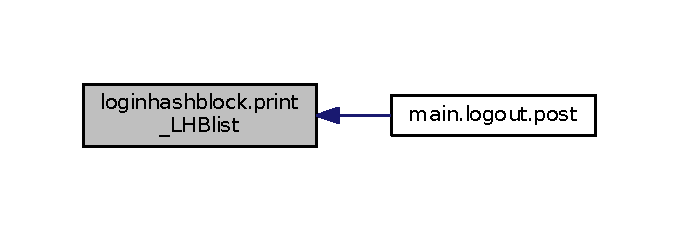
\includegraphics[width=326pt]{namespaceloginhashblock_a1096aa8494b9c5875decc029d8b40ea9_icgraph}
\end{center}
\end{figure}


\index{loginhashblock@{loginhashblock}!update\+\_\+loginhashblock@{update\+\_\+loginhashblock}}
\index{update\+\_\+loginhashblock@{update\+\_\+loginhashblock}!loginhashblock@{loginhashblock}}
\subsubsection[{\texorpdfstring{update\+\_\+loginhashblock(prev\+L\+H\+Bstr, D\+E\+B\+U\+G=\+False)}{update_loginhashblock(prevLHBstr, DEBUG=False)}}]{\setlength{\rightskip}{0pt plus 5cm}def loginhashblock.\+update\+\_\+loginhashblock (
\begin{DoxyParamCaption}
\item[{}]{prev\+L\+H\+Bstr, }
\item[{}]{D\+E\+B\+UG = {\ttfamily False}}
\end{DoxyParamCaption}
)}\hypertarget{namespaceloginhashblock_afef75d97c834ce0fda711b93d0b56b00}{}\label{namespaceloginhashblock_afef75d97c834ce0fda711b93d0b56b00}
\begin{DoxyVerb}This function is to update login hash block with old login hash block
:param prevLHBstr:
:param DEBUG:
:return: updated login hash block
\end{DoxyVerb}
 

Definition at line 315 of file loginhashblock.\+py.


\begin{DoxyCode}
315 \textcolor{keyword}{def }\hyperlink{namespaceloginhashblock_afef75d97c834ce0fda711b93d0b56b00}{update\_loginhashblock}(prevLHBstr, DEBUG=False):
316     \textcolor{stringliteral}{"""}
317 \textcolor{stringliteral}{    This function is to update login hash block with old login hash block}
318 \textcolor{stringliteral}{    :param prevLHBstr:}
319 \textcolor{stringliteral}{    :param DEBUG:}
320 \textcolor{stringliteral}{    :return: updated login hash block}
321 \textcolor{stringliteral}{    """}
322 
323     \textcolor{keywordflow}{if} \textcolor{keywordflow}{not} prevLHBstr:
324         \textcolor{keywordflow}{return} \textcolor{keywordtype}{None}
325 
326     \textcolor{keywordflow}{if} \textcolor{keywordflow}{not} \hyperlink{namespaceloginhashblock_adb424539d851426da7b65d53c5a6d577}{valid\_loginhashblock}(prevLHBstr, DEBUG=DEBUG):
327         \textcolor{keywordflow}{raise} ValueError(\textcolor{stringliteral}{"[info:update\_loginhashblock] Invalid login hash block"})
328 
329     devid = \hyperlink{namespaceloginhashblock_a17417f2f6bca76ab51170082a562e5f6}{get\_deviceId}(prevLHBstr, DEBUG=DEBUG)
330     LHBstr = \hyperlink{namespaceloginhashblock_ad3ef8dab740c69ca8424797f9c146a53}{create\_loginhashblock}(devid, DEBUG=DEBUG)
331 
332     \textcolor{keywordflow}{if} DEBUG:
333         text = \textcolor{stringliteral}{'[info:update\_loginhashblock] \(\backslash\)npre\_loginhashblock: \{\}\(\backslash\)nnew\_loginhashblock: \{\}'}.format(
      prevLHBstr,LHBstr)
334         print(text)
335 
336     \textcolor{keywordflow}{return} LHBstr
337 
\end{DoxyCode}


Here is the call graph for this function\+:
\nopagebreak
\begin{figure}[H]
\begin{center}
\leavevmode
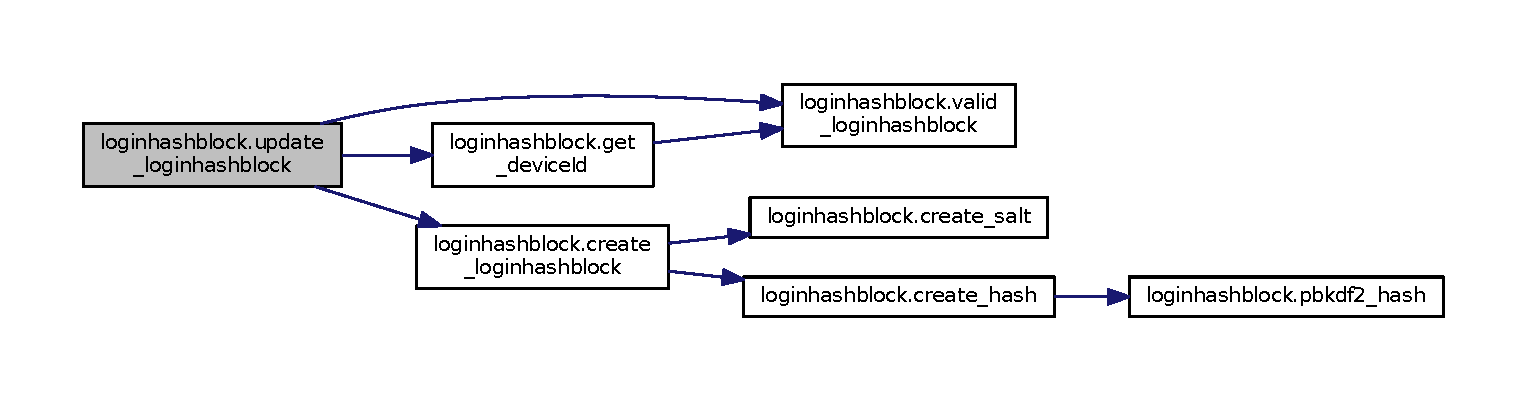
\includegraphics[width=350pt]{namespaceloginhashblock_afef75d97c834ce0fda711b93d0b56b00_cgraph}
\end{center}
\end{figure}




Here is the caller graph for this function\+:
\nopagebreak
\begin{figure}[H]
\begin{center}
\leavevmode
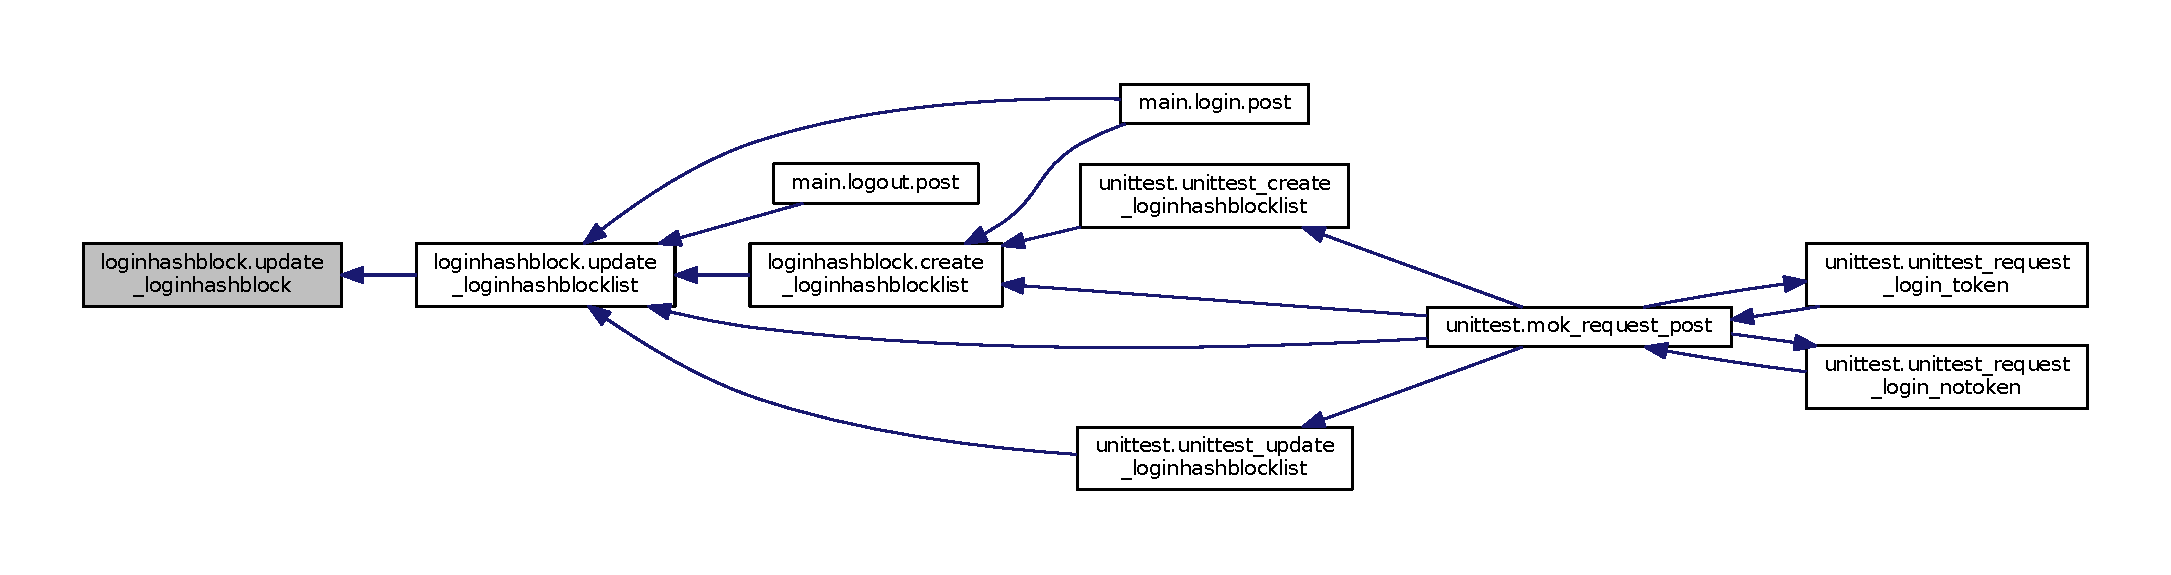
\includegraphics[width=350pt]{namespaceloginhashblock_afef75d97c834ce0fda711b93d0b56b00_icgraph}
\end{center}
\end{figure}


\index{loginhashblock@{loginhashblock}!update\+\_\+loginhashblocklist@{update\+\_\+loginhashblocklist}}
\index{update\+\_\+loginhashblocklist@{update\+\_\+loginhashblocklist}!loginhashblock@{loginhashblock}}
\subsubsection[{\texorpdfstring{update\+\_\+loginhashblocklist(\+L\+H\+Blist\+Str, prev\+L\+H\+Bstr, D\+E\+B\+U\+G=\+False)}{update_loginhashblocklist(LHBlistStr, prevLHBstr, DEBUG=False)}}]{\setlength{\rightskip}{0pt plus 5cm}def loginhashblock.\+update\+\_\+loginhashblocklist (
\begin{DoxyParamCaption}
\item[{}]{L\+H\+Blist\+Str, }
\item[{}]{prev\+L\+H\+Bstr, }
\item[{}]{D\+E\+B\+UG = {\ttfamily False}}
\end{DoxyParamCaption}
)}\hypertarget{namespaceloginhashblock_a2bcc7ddd0fcc3788572dd77808cb624d}{}\label{namespaceloginhashblock_a2bcc7ddd0fcc3788572dd77808cb624d}
\begin{DoxyVerb}This function update login hash block list.
:param LHBlistStr: login hash block list string
:param LHBstr: login hash block
:return:
\end{DoxyVerb}
 

Definition at line 97 of file loginhashblock.\+py.


\begin{DoxyCode}
97 \textcolor{keyword}{def }\hyperlink{namespaceloginhashblock_a2bcc7ddd0fcc3788572dd77808cb624d}{update\_loginhashblocklist}(LHBlistStr, prevLHBstr, DEBUG=False):
98     \textcolor{stringliteral}{"""}
99 \textcolor{stringliteral}{    This function update login hash block list.}
100 \textcolor{stringliteral}{    :param LHBlistStr: login hash block list string}
101 \textcolor{stringliteral}{    :param LHBstr: login hash block}
102 \textcolor{stringliteral}{    :return:}
103 \textcolor{stringliteral}{    """}
104 
105     LHBstr = \hyperlink{namespaceloginhashblock_afef75d97c834ce0fda711b93d0b56b00}{update\_loginhashblock}(prevLHBstr, DEBUG=\textcolor{keyword}{False})
106 
107     \textcolor{keywordflow}{if} \textcolor{keywordflow}{not} LHBstr:
108         \textcolor{keywordflow}{return} LHBlistStr, LHBstr
109 
110     devid = \hyperlink{namespaceloginhashblock_a17417f2f6bca76ab51170082a562e5f6}{get\_deviceId}(LHBstr, DEBUG=DEBUG)
111 
112     \textcolor{keywordflow}{if} \textcolor{keywordflow}{not} LHBlistStr:
113         LHBlistStr = LHBstr
114         
115         \textcolor{keywordflow}{if} DEBUG:
116             print(\textcolor{stringliteral}{"[info:update\_loginhashblocklist] LHBlistStr is null"})
117 
118         \textcolor{keywordflow}{return} LHBlistStr, LHBstr
119 
120     LHBlist = LHBlistStr.split(\textcolor{stringliteral}{','})
121 
122     \textcolor{keywordflow}{for} i,v \textcolor{keywordflow}{in} enumerate(LHBlist):
123         \_devid = \hyperlink{namespaceloginhashblock_a17417f2f6bca76ab51170082a562e5f6}{get\_deviceId}(v, DEBUG=DEBUG)
124         \textcolor{keywordflow}{if} devid == \_devid:
125             LHBlist[i] = LHBstr
126             LHBlistStr = \textcolor{stringliteral}{","}.join(LHBlist)
127             \textcolor{keywordflow}{return} LHBlistStr, LHBstr
128 
129     LHBlist.append(LHBstr)
130 
131     \textcolor{keywordflow}{if} DEBUG:
132         print(\textcolor{stringliteral}{"[info:update\_loginhashblocklist] devid: \{\}"}.format(devid))
133         print(\textcolor{stringliteral}{"[info:update\_loginhashblocklist] db\_hashblock: \{\}"}.format(len(LHBlist)))
134 
135     LHBlistStr = \textcolor{stringliteral}{","}.join(LHBlist)
136 
137     \textcolor{keywordflow}{return} LHBlistStr, LHBstr
138 
\end{DoxyCode}


Here is the call graph for this function\+:
\nopagebreak
\begin{figure}[H]
\begin{center}
\leavevmode
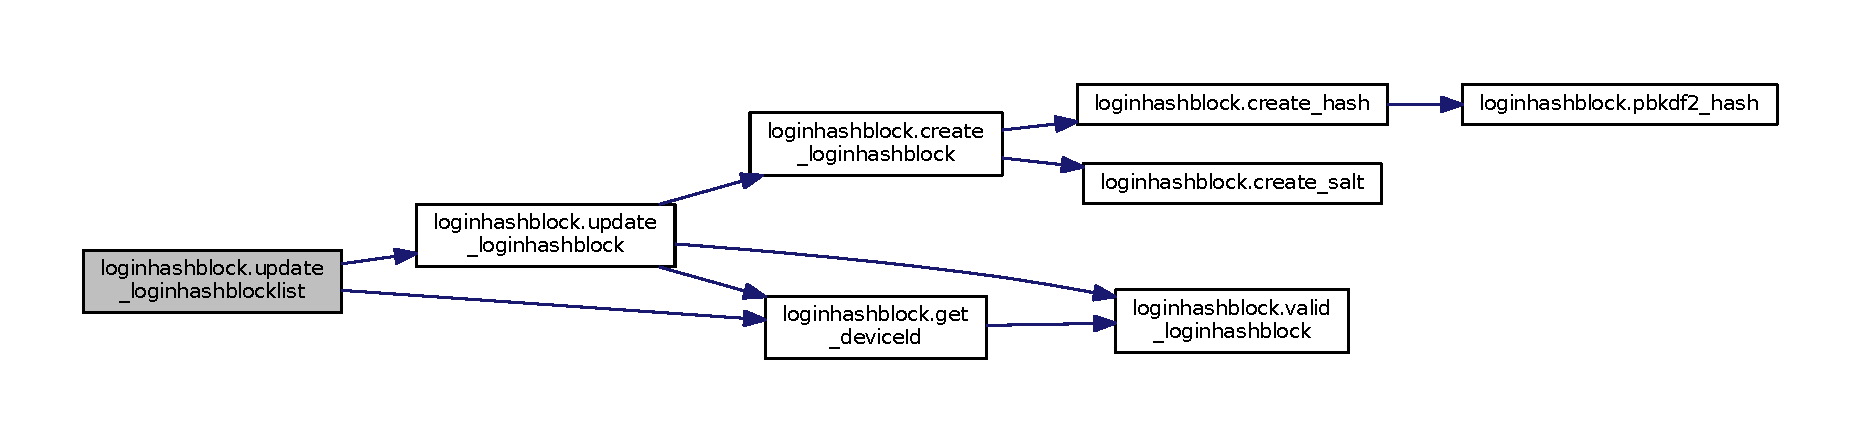
\includegraphics[width=350pt]{namespaceloginhashblock_a2bcc7ddd0fcc3788572dd77808cb624d_cgraph}
\end{center}
\end{figure}




Here is the caller graph for this function\+:
\nopagebreak
\begin{figure}[H]
\begin{center}
\leavevmode
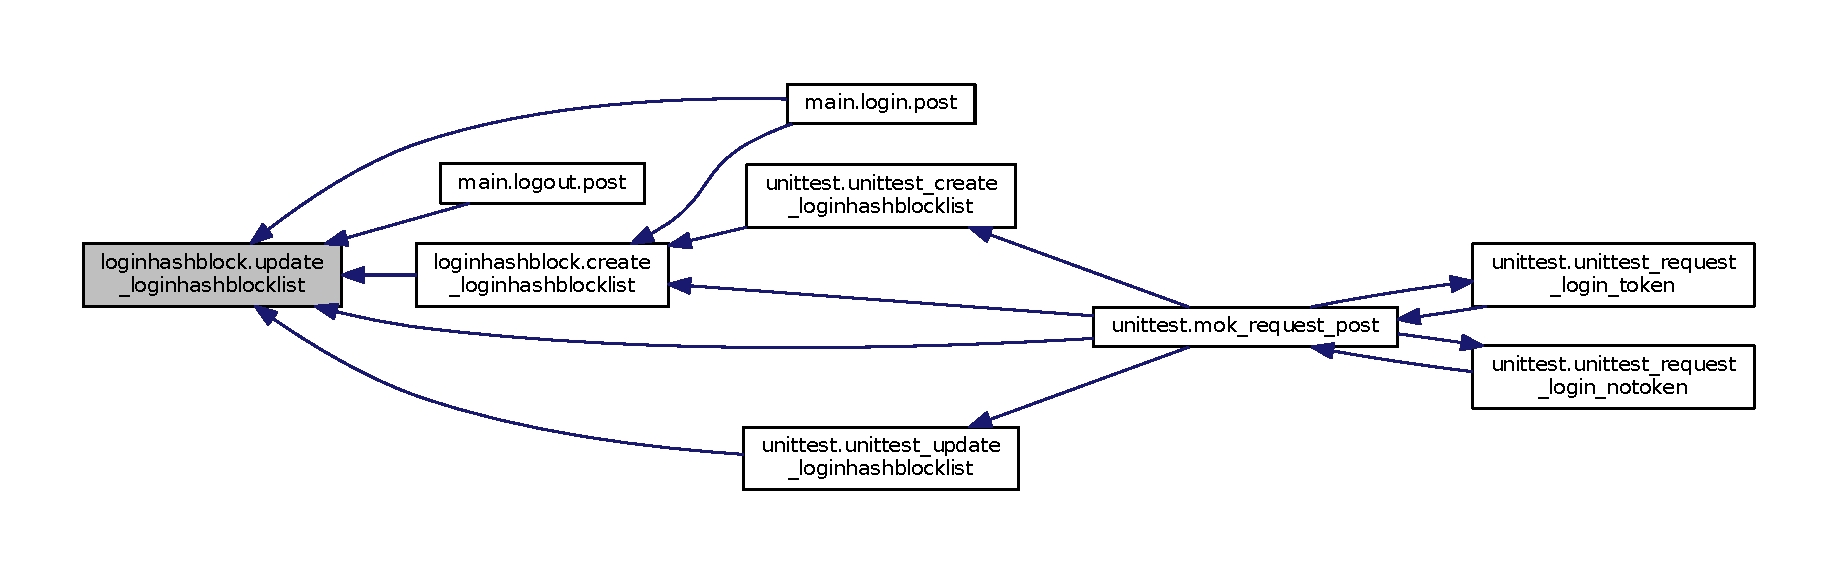
\includegraphics[width=350pt]{namespaceloginhashblock_a2bcc7ddd0fcc3788572dd77808cb624d_icgraph}
\end{center}
\end{figure}


\index{loginhashblock@{loginhashblock}!valid\+\_\+hash@{valid\+\_\+hash}}
\index{valid\+\_\+hash@{valid\+\_\+hash}!loginhashblock@{loginhashblock}}
\subsubsection[{\texorpdfstring{valid\+\_\+hash(target\+\_\+hash, salt, target, method, D\+E\+B\+U\+G=\+False)}{valid_hash(target_hash, salt, target, method, DEBUG=False)}}]{\setlength{\rightskip}{0pt plus 5cm}def loginhashblock.\+valid\+\_\+hash (
\begin{DoxyParamCaption}
\item[{}]{target\+\_\+hash, }
\item[{}]{salt, }
\item[{}]{target, }
\item[{}]{method, }
\item[{}]{D\+E\+B\+UG = {\ttfamily False}}
\end{DoxyParamCaption}
)}\hypertarget{namespaceloginhashblock_ac7faa165bc305e611390727f11946424}{}\label{namespaceloginhashblock_ac7faa165bc305e611390727f11946424}
\begin{DoxyVerb}This function is to check hash block
:param target_hash:
:param salt:
:param target:
:param method:
:return:
\end{DoxyVerb}
 

Definition at line 172 of file loginhashblock.\+py.


\begin{DoxyCode}
172 \textcolor{keyword}{def }\hyperlink{namespaceloginhashblock_ac7faa165bc305e611390727f11946424}{valid\_hash}(target\_hash, salt, target, method, DEBUG=False):
173     \textcolor{stringliteral}{"""}
174 \textcolor{stringliteral}{    This function is to check hash block}
175 \textcolor{stringliteral}{    :param target\_hash:}
176 \textcolor{stringliteral}{    :param salt:}
177 \textcolor{stringliteral}{    :param target:}
178 \textcolor{stringliteral}{    :param method:}
179 \textcolor{stringliteral}{    :return:}
180 \textcolor{stringliteral}{    """}
181 
182     \textcolor{keywordflow}{if} method.count(\textcolor{stringliteral}{":"}) != 2:
183         \textcolor{keywordflow}{return} \textcolor{keyword}{False}
184 
185     kdf, hash\_name, iterations = method.split(\textcolor{stringliteral}{":"}, 2)
186     hash, method = \hyperlink{namespaceloginhashblock_a935d8ae1c51e50f9e5db6a1d5f02b1b8}{create\_hash}(salt, target, hash\_name=hash\_name, iterations=int(iterations), 
      kdf=kdf)
187     ret = \hyperlink{namespaceloginhashblock_ac24dd842eb90e0ede55e842d44148d5b}{compare\_loginhashblock}(hash, target\_hash)
188 
189     \textcolor{keywordflow}{if} DEBUG:
190         print(\textcolor{stringliteral}{"[info:valid\_hash]        hash: "}, hash)
191         print(\textcolor{stringliteral}{"[info:valid\_hash] target\_hash: "}, target\_hash)
192         print(\textcolor{stringliteral}{"[info:valid\_hash]         ret: "}, ret)
193 
194     \textcolor{keywordflow}{return} ret
195 
\end{DoxyCode}


Here is the call graph for this function\+:
\nopagebreak
\begin{figure}[H]
\begin{center}
\leavevmode
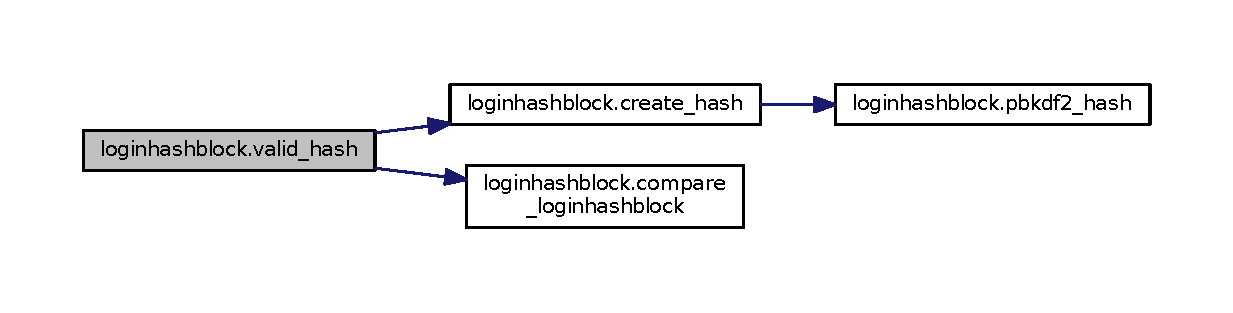
\includegraphics[width=350pt]{namespaceloginhashblock_ac7faa165bc305e611390727f11946424_cgraph}
\end{center}
\end{figure}


\index{loginhashblock@{loginhashblock}!valid\+\_\+loginhashblock@{valid\+\_\+loginhashblock}}
\index{valid\+\_\+loginhashblock@{valid\+\_\+loginhashblock}!loginhashblock@{loginhashblock}}
\subsubsection[{\texorpdfstring{valid\+\_\+loginhashblock(\+L\+H\+Bstr, D\+E\+B\+U\+G=\+False)}{valid_loginhashblock(LHBstr, DEBUG=False)}}]{\setlength{\rightskip}{0pt plus 5cm}def loginhashblock.\+valid\+\_\+loginhashblock (
\begin{DoxyParamCaption}
\item[{}]{L\+H\+Bstr, }
\item[{}]{D\+E\+B\+UG = {\ttfamily False}}
\end{DoxyParamCaption}
)}\hypertarget{namespaceloginhashblock_adb424539d851426da7b65d53c5a6d577}{}\label{namespaceloginhashblock_adb424539d851426da7b65d53c5a6d577}
\begin{DoxyVerb}This function is to check login hash block
hashblock format: deviceid(8)+$+hash
ex)jUs6LQMX$jUs6LQMX$ceccffbfa52e55825f87573b068c8d759b1540f9833a7d7ebd7a27c993ffd316
:param LHBstr:
:return: BOOL
\end{DoxyVerb}
 

Definition at line 282 of file loginhashblock.\+py.


\begin{DoxyCode}
282 \textcolor{keyword}{def }\hyperlink{namespaceloginhashblock_adb424539d851426da7b65d53c5a6d577}{valid\_loginhashblock}(LHBstr, DEBUG=False):
283     \textcolor{stringliteral}{"""}
284 \textcolor{stringliteral}{    This function is to check login hash block}
285 \textcolor{stringliteral}{    hashblock format: deviceid(8)+$+hash}
286 \textcolor{stringliteral}{    ex)jUs6LQMX$jUs6LQMX$ceccffbfa52e55825f87573b068c8d759b1540f9833a7d7ebd7a27c993ffd316}
287 \textcolor{stringliteral}{    :param LHBstr:}
288 \textcolor{stringliteral}{    :return: BOOL}
289 \textcolor{stringliteral}{    """}
290     \textcolor{keywordflow}{if} \textcolor{keywordflow}{not} LHBstr:
291         \textcolor{keywordflow}{if} DEBUG:
292             print(\textcolor{stringliteral}{'[info:valid\_loginhashblock] Null'})
293         \textcolor{keywordflow}{return} \textcolor{keyword}{False}
294 
295     \textcolor{keywordflow}{if} LHBstr.count(\textcolor{stringliteral}{"$"}) != 1:
296         \textcolor{keywordflow}{if} DEBUG:
297             print(\textcolor{stringliteral}{'[info:valid\_loginhashblock] Invalid format'})
298         \textcolor{keywordflow}{return} \textcolor{keyword}{False}
299 
300     devid, hash = LHBstr.split(\textcolor{stringliteral}{"$"}, 1)
301 
302     \textcolor{keywordflow}{if} len(devid) != 8:
303         \textcolor{keywordflow}{if} DEBUG:
304             print(\textcolor{stringliteral}{'[info:valid\_loginhashblock] Invalid deviceid'})
305         \textcolor{keywordflow}{return} \textcolor{keyword}{False}
306 
307     \textcolor{keywordflow}{if} len(hash) != 64:
308         \textcolor{keywordflow}{return} \textcolor{keyword}{False}
309 
310     \textcolor{keywordflow}{if} DEBUG:
311         print(\textcolor{stringliteral}{'[info:valid\_loginhashblock] login hash block is valid'})
312 
313     \textcolor{keywordflow}{return} \textcolor{keyword}{True}
314 
\end{DoxyCode}


Here is the caller graph for this function\+:
\nopagebreak
\begin{figure}[H]
\begin{center}
\leavevmode
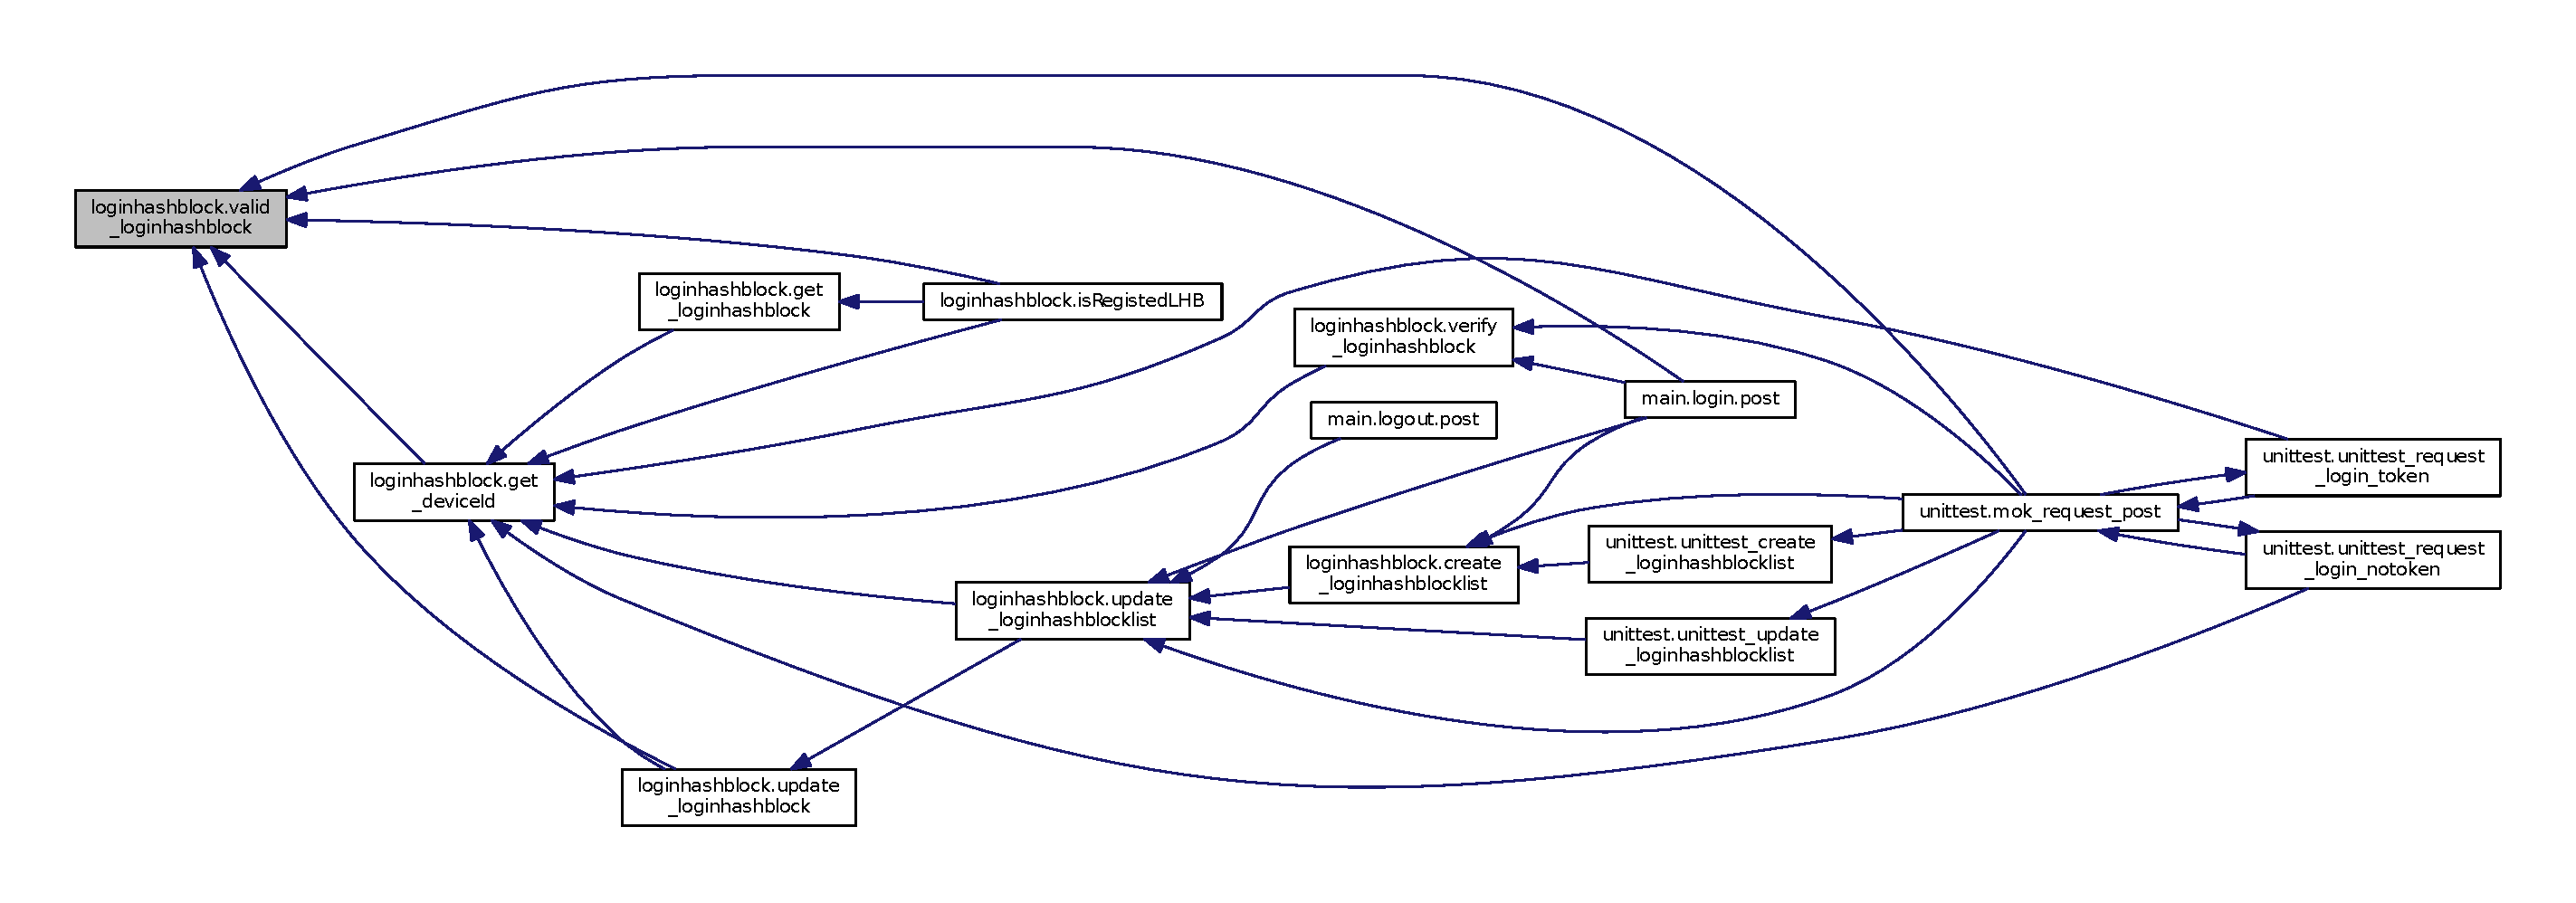
\includegraphics[width=350pt]{namespaceloginhashblock_adb424539d851426da7b65d53c5a6d577_icgraph}
\end{center}
\end{figure}


\index{loginhashblock@{loginhashblock}!verify\+\_\+loginhashblock@{verify\+\_\+loginhashblock}}
\index{verify\+\_\+loginhashblock@{verify\+\_\+loginhashblock}!loginhashblock@{loginhashblock}}
\subsubsection[{\texorpdfstring{verify\+\_\+loginhashblock(\+L\+H\+Blist\+Str, L\+H\+Bstr, D\+E\+B\+U\+G=\+False)}{verify_loginhashblock(LHBlistStr, LHBstr, DEBUG=False)}}]{\setlength{\rightskip}{0pt plus 5cm}def loginhashblock.\+verify\+\_\+loginhashblock (
\begin{DoxyParamCaption}
\item[{}]{L\+H\+Blist\+Str, }
\item[{}]{L\+H\+Bstr, }
\item[{}]{D\+E\+B\+UG = {\ttfamily False}}
\end{DoxyParamCaption}
)}\hypertarget{namespaceloginhashblock_aa5bb94484a68d0bbebce23b4cfeeb4b7}{}\label{namespaceloginhashblock_aa5bb94484a68d0bbebce23b4cfeeb4b7}
\begin{DoxyVerb}This function verify login hash block list.
:param LHBlistStr: login hash block list
:param LHBstr: login hash block
:return:
\end{DoxyVerb}
 

Definition at line 258 of file loginhashblock.\+py.


\begin{DoxyCode}
258 \textcolor{keyword}{def }\hyperlink{namespaceloginhashblock_aa5bb94484a68d0bbebce23b4cfeeb4b7}{verify\_loginhashblock}(LHBlistStr, LHBstr, DEBUG=False):
259     \textcolor{stringliteral}{"""}
260 \textcolor{stringliteral}{    This function verify login hash block list.}
261 \textcolor{stringliteral}{    :param LHBlistStr: login hash block list}
262 \textcolor{stringliteral}{    :param LHBstr: login hash block}
263 \textcolor{stringliteral}{    :return:}
264 \textcolor{stringliteral}{    """}
265 
266     \textcolor{keywordflow}{if} \textcolor{keywordflow}{not} LHBlistStr :
267         \textcolor{keywordflow}{return} \textcolor{keyword}{False}
268 
269     devid = \hyperlink{namespaceloginhashblock_a17417f2f6bca76ab51170082a562e5f6}{get\_deviceId}(LHBstr, DEBUG=DEBUG)
270     LHBlist = LHBlistStr.split(\textcolor{stringliteral}{','})
271 
272     \textcolor{keywordflow}{for} i,v \textcolor{keywordflow}{in} enumerate(LHBlist):
273         \_devid = \hyperlink{namespaceloginhashblock_a17417f2f6bca76ab51170082a562e5f6}{get\_deviceId}(v, DEBUG=DEBUG)
274         \textcolor{keywordflow}{if} devid == \_devid:
275             \textcolor{keywordflow}{if} v == LHBstr:
276                 \textcolor{keywordflow}{return} \textcolor{keyword}{True}
277             \textcolor{keywordflow}{else}:
278                 \textcolor{keywordflow}{return} \textcolor{keyword}{False}
279 
280     \textcolor{keywordflow}{return} \textcolor{keyword}{False}
281 
\end{DoxyCode}


Here is the call graph for this function\+:
\nopagebreak
\begin{figure}[H]
\begin{center}
\leavevmode
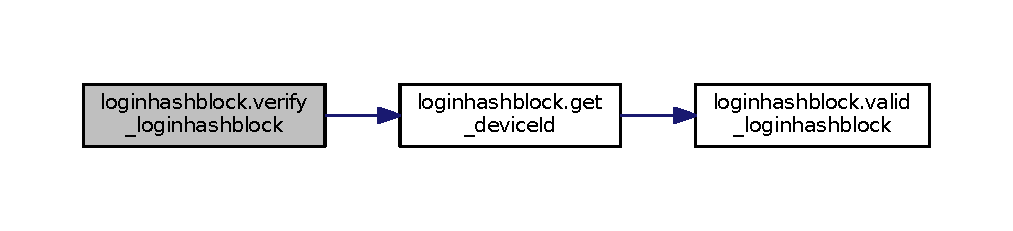
\includegraphics[width=350pt]{namespaceloginhashblock_aa5bb94484a68d0bbebce23b4cfeeb4b7_cgraph}
\end{center}
\end{figure}




Here is the caller graph for this function\+:
\nopagebreak
\begin{figure}[H]
\begin{center}
\leavevmode
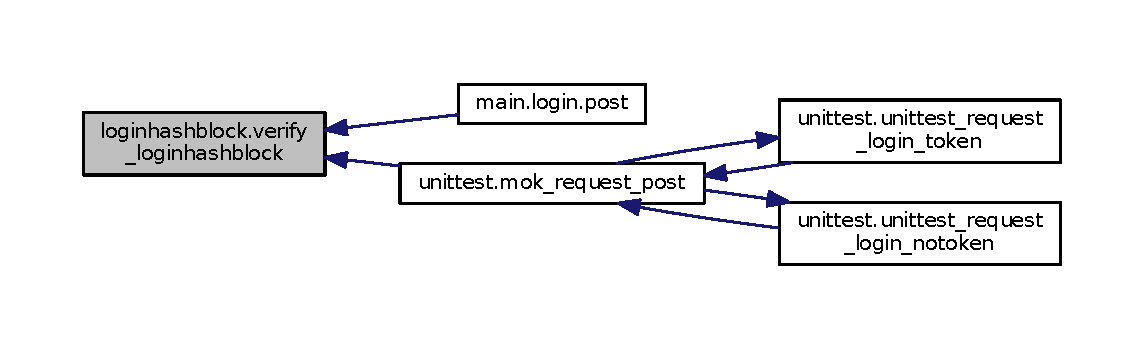
\includegraphics[width=350pt]{namespaceloginhashblock_aa5bb94484a68d0bbebce23b4cfeeb4b7_icgraph}
\end{center}
\end{figure}




\subsection{Variable Documentation}
\index{loginhashblock@{loginhashblock}!D\+E\+B\+UG@{D\+E\+B\+UG}}
\index{D\+E\+B\+UG@{D\+E\+B\+UG}!loginhashblock@{loginhashblock}}
\subsubsection[{\texorpdfstring{D\+E\+B\+UG}{DEBUG}}]{\setlength{\rightskip}{0pt plus 5cm}bool loginhashblock.\+D\+E\+B\+UG = False}\hypertarget{namespaceloginhashblock_ad198a2ffc3d7bab32167aed00d2f5c65}{}\label{namespaceloginhashblock_ad198a2ffc3d7bab32167aed00d2f5c65}


Definition at line 18 of file loginhashblock.\+py.


\hypertarget{namespacemain}{}\doxysection{main Namespace Reference}
\label{namespacemain}\index{main@{main}}
\doxysubsection*{Classes}
\begin{DoxyCompactItemize}
\item 
class \mbox{\hyperlink{classmain_1_1command}{command}}
\item 
class \mbox{\hyperlink{classmain_1_1index}{index}}
\item 
class \mbox{\hyperlink{classmain_1_1login}{login}}
\item 
class \mbox{\hyperlink{classmain_1_1logout}{logout}}
\item 
class \mbox{\hyperlink{classmain_1_1qrcode}{qrcode}}
\item 
class \mbox{\hyperlink{classmain_1_1register}{register}}
\item 
class \mbox{\hyperlink{classmain_1_1RegisterForm}{Register\+Form}}
\item 
class \mbox{\hyperlink{classmain_1_1twofactor}{twofactor}}
\item 
class \mbox{\hyperlink{classmain_1_1User}{User}}
\end{DoxyCompactItemize}
\doxysubsection*{Functions}
\begin{DoxyCompactItemize}
\item 
def \mbox{\hyperlink{namespacemain_a64310d76bee3c7581aaa85925bf1bb53}{load\+\_\+user}} (user\+\_\+id)
\item 
def \mbox{\hyperlink{namespacemain_a0803c7dc3e1c168a3fbcf5b054109aa1}{not\+\_\+found}} (e)
\end{DoxyCompactItemize}
\doxysubsection*{Variables}
\begin{DoxyCompactItemize}
\item 
bool \mbox{\hyperlink{namespacemain_ad2cce3c3d1036d38f161e4814c97e1b5}{D\+E\+B\+UG}} = False
\item 
\mbox{\hyperlink{namespacemain_a5fa94f0581009434c7a63791944d6ff4}{app}} = Flask(\+\_\+\+\_\+name\+\_\+\+\_\+)
\item 
\mbox{\hyperlink{namespacemain_a2f0b4b807236469879d595c7f18850aa}{api}} = Api(\mbox{\hyperlink{namespacemain_a5fa94f0581009434c7a63791944d6ff4}{app}})
\item 
\mbox{\hyperlink{namespacemain_a2799db3c64165e5659fada6c15d90aea}{bootstrap}} = Bootstrap(\mbox{\hyperlink{namespacemain_a5fa94f0581009434c7a63791944d6ff4}{app}})
\item 
\mbox{\hyperlink{namespacemain_afadee2a30284fe18a4fee574c23c94e3}{db}} = S\+Q\+L\+Alchemy(\mbox{\hyperlink{namespacemain_a5fa94f0581009434c7a63791944d6ff4}{app}})
\item 
\mbox{\hyperlink{namespacemain_aaf584fa2bbd608ba30fe2a84f4a6e604}{lm}} = Login\+Manager(\mbox{\hyperlink{namespacemain_a5fa94f0581009434c7a63791944d6ff4}{app}})
\end{DoxyCompactItemize}


\doxysubsection{Detailed Description}
\begin{DoxyVerb}This is example web site using python flask based on LHB(login hash block) module.
@version: 1.0.0
@authour: suwonchon(suwonchon@gmail.com)
@contact http://github.com/masuwonchon/loginblockchain
@license: MIT
\end{DoxyVerb}
 

\doxysubsection{Function Documentation}
\mbox{\Hypertarget{namespacemain_a64310d76bee3c7581aaa85925bf1bb53}\label{namespacemain_a64310d76bee3c7581aaa85925bf1bb53}} 
\index{main@{main}!load\_user@{load\_user}}
\index{load\_user@{load\_user}!main@{main}}
\doxysubsubsection{\texorpdfstring{load\_user()}{load\_user()}}
{\footnotesize\ttfamily def main.\+load\+\_\+user (\begin{DoxyParamCaption}\item[{}]{user\+\_\+id }\end{DoxyParamCaption})}

\begin{DoxyVerb}User loader callback for Flask-Login.\end{DoxyVerb}
 

Definition at line 79 of file main.\+py.


\begin{DoxyCode}{0}
\DoxyCodeLine{79 \textcolor{keyword}{def }\mbox{\hyperlink{namespacemain_a64310d76bee3c7581aaa85925bf1bb53}{load\_user}}(user\_id):}
\DoxyCodeLine{80     \textcolor{stringliteral}{"""User loader callback for Flask-\/Login."""}}
\DoxyCodeLine{81     \textcolor{keywordflow}{return} User.query.get(int(user\_id))}
\DoxyCodeLine{82 }

\end{DoxyCode}
\mbox{\Hypertarget{namespacemain_a0803c7dc3e1c168a3fbcf5b054109aa1}\label{namespacemain_a0803c7dc3e1c168a3fbcf5b054109aa1}} 
\index{main@{main}!not\_found@{not\_found}}
\index{not\_found@{not\_found}!main@{main}}
\doxysubsubsection{\texorpdfstring{not\_found()}{not\_found()}}
{\footnotesize\ttfamily def main.\+not\+\_\+found (\begin{DoxyParamCaption}\item[{}]{e }\end{DoxyParamCaption})}



Definition at line 313 of file main.\+py.


\begin{DoxyCode}{0}
\DoxyCodeLine{313 \textcolor{keyword}{def }\mbox{\hyperlink{namespacemain_a0803c7dc3e1c168a3fbcf5b054109aa1}{not\_found}}(e):}
\DoxyCodeLine{314     \textcolor{keywordflow}{return} \textcolor{stringliteral}{''}, 404}
\DoxyCodeLine{315 }

\end{DoxyCode}


\doxysubsection{Variable Documentation}
\mbox{\Hypertarget{namespacemain_a2f0b4b807236469879d595c7f18850aa}\label{namespacemain_a2f0b4b807236469879d595c7f18850aa}} 
\index{main@{main}!api@{api}}
\index{api@{api}!main@{main}}
\doxysubsubsection{\texorpdfstring{api}{api}}
{\footnotesize\ttfamily main.\+api = Api(\mbox{\hyperlink{namespacemain_a5fa94f0581009434c7a63791944d6ff4}{app}})}



Definition at line 33 of file main.\+py.

\mbox{\Hypertarget{namespacemain_a5fa94f0581009434c7a63791944d6ff4}\label{namespacemain_a5fa94f0581009434c7a63791944d6ff4}} 
\index{main@{main}!app@{app}}
\index{app@{app}!main@{main}}
\doxysubsubsection{\texorpdfstring{app}{app}}
{\footnotesize\ttfamily main.\+app = Flask(\+\_\+\+\_\+name\+\_\+\+\_\+)}



Definition at line 32 of file main.\+py.

\mbox{\Hypertarget{namespacemain_a2799db3c64165e5659fada6c15d90aea}\label{namespacemain_a2799db3c64165e5659fada6c15d90aea}} 
\index{main@{main}!bootstrap@{bootstrap}}
\index{bootstrap@{bootstrap}!main@{main}}
\doxysubsubsection{\texorpdfstring{bootstrap}{bootstrap}}
{\footnotesize\ttfamily main.\+bootstrap = Bootstrap(\mbox{\hyperlink{namespacemain_a5fa94f0581009434c7a63791944d6ff4}{app}})}



Definition at line 37 of file main.\+py.

\mbox{\Hypertarget{namespacemain_afadee2a30284fe18a4fee574c23c94e3}\label{namespacemain_afadee2a30284fe18a4fee574c23c94e3}} 
\index{main@{main}!db@{db}}
\index{db@{db}!main@{main}}
\doxysubsubsection{\texorpdfstring{db}{db}}
{\footnotesize\ttfamily main.\+db = S\+Q\+L\+Alchemy(\mbox{\hyperlink{namespacemain_a5fa94f0581009434c7a63791944d6ff4}{app}})}



Definition at line 38 of file main.\+py.

\mbox{\Hypertarget{namespacemain_ad2cce3c3d1036d38f161e4814c97e1b5}\label{namespacemain_ad2cce3c3d1036d38f161e4814c97e1b5}} 
\index{main@{main}!DEBUG@{DEBUG}}
\index{DEBUG@{DEBUG}!main@{main}}
\doxysubsubsection{\texorpdfstring{DEBUG}{DEBUG}}
{\footnotesize\ttfamily bool main.\+D\+E\+B\+UG = False}



Definition at line 29 of file main.\+py.

\mbox{\Hypertarget{namespacemain_aaf584fa2bbd608ba30fe2a84f4a6e604}\label{namespacemain_aaf584fa2bbd608ba30fe2a84f4a6e604}} 
\index{main@{main}!lm@{lm}}
\index{lm@{lm}!main@{main}}
\doxysubsubsection{\texorpdfstring{lm}{lm}}
{\footnotesize\ttfamily main.\+lm = Login\+Manager(\mbox{\hyperlink{namespacemain_a5fa94f0581009434c7a63791944d6ff4}{app}})}



Definition at line 39 of file main.\+py.


\hypertarget{namespacerun}{}\doxysection{run Namespace Reference}
\label{namespacerun}\index{run@{run}}
\doxysubsection*{Variables}
\begin{DoxyCompactItemize}
\item 
\mbox{\hyperlink{namespacerun_a24785e11198aac41f0051e51857331aa}{debug}}
\item 
\mbox{\hyperlink{namespacerun_af7767eb404b922097d7206695c016bad}{host}} = os.\+environ.\+get(\textquotesingle{}IP\textquotesingle{}, \textquotesingle{}0.\+0.\+0.\+0\textquotesingle{})
\item 
\mbox{\hyperlink{namespacerun_a7a6a5c33b9e900b36c2b941d5212210e}{port}} = int(os.\+environ.\+get(\textquotesingle{}P\+O\+RT\textquotesingle{}, 80))
\end{DoxyCompactItemize}


\doxysubsection{Detailed Description}
\begin{DoxyVerb}This is example web site using python flask based on LHB(login hash block) module.
@version: 1.0.0
@authour: suwonchon(suwonchon@gmail.com)
@contact http://github.com/masuwonchon/loginblockchain
@license: MIT
\end{DoxyVerb}
 

\doxysubsection{Variable Documentation}
\mbox{\Hypertarget{namespacerun_a24785e11198aac41f0051e51857331aa}\label{namespacerun_a24785e11198aac41f0051e51857331aa}} 
\index{run@{run}!debug@{debug}}
\index{debug@{debug}!run@{run}}
\doxysubsubsection{\texorpdfstring{debug}{debug}}
{\footnotesize\ttfamily run.\+debug}



Definition at line 13 of file run.\+py.

\mbox{\Hypertarget{namespacerun_af7767eb404b922097d7206695c016bad}\label{namespacerun_af7767eb404b922097d7206695c016bad}} 
\index{run@{run}!host@{host}}
\index{host@{host}!run@{run}}
\doxysubsubsection{\texorpdfstring{host}{host}}
{\footnotesize\ttfamily run.\+host = os.\+environ.\+get(\textquotesingle{}IP\textquotesingle{}, \textquotesingle{}0.\+0.\+0.\+0\textquotesingle{})}



Definition at line 14 of file run.\+py.

\mbox{\Hypertarget{namespacerun_a7a6a5c33b9e900b36c2b941d5212210e}\label{namespacerun_a7a6a5c33b9e900b36c2b941d5212210e}} 
\index{run@{run}!port@{port}}
\index{port@{port}!run@{run}}
\doxysubsubsection{\texorpdfstring{port}{port}}
{\footnotesize\ttfamily run.\+port = int(os.\+environ.\+get(\textquotesingle{}P\+O\+RT\textquotesingle{}, 80))}



Definition at line 15 of file run.\+py.


\hypertarget{namespaceunittest}{}\section{unittest Namespace Reference}
\label{namespaceunittest}\index{unittest@{unittest}}
\subsection*{Classes}
\begin{DoxyCompactItemize}
\item 
class \hyperlink{classunittest_1_1bcolors}{bcolors}
\end{DoxyCompactItemize}
\subsection*{Functions}
\begin{DoxyCompactItemize}
\item 
def \hyperlink{namespaceunittest_a217a1a3af5bc9748f2f6194bf79402bc}{unittest\+\_\+print} (message)
\item 
def \hyperlink{namespaceunittest_a642ec5401fe406315f1489d237ba826e}{unittest\+\_\+title\+\_\+print} (message)
\item 
def \hyperlink{namespaceunittest_a9e16eaba67b93461be6ea8ef6332507a}{unittest\+\_\+update\+\_\+loginhashblocklist} ()
\item 
def \hyperlink{namespaceunittest_a0e10bea14aac2cc6a08d76f422b9328d}{unittest\+\_\+create\+\_\+loginhashblocklist} ()
\end{DoxyCompactItemize}
\subsection*{Variables}
\begin{DoxyCompactItemize}
\item 
bool \hyperlink{namespaceunittest_a6f95c254ae4668ea73efe6cf7ca3c36d}{D\+E\+B\+UG} = False
\end{DoxyCompactItemize}


\subsection{Function Documentation}
\index{unittest@{unittest}!unittest\+\_\+create\+\_\+loginhashblocklist@{unittest\+\_\+create\+\_\+loginhashblocklist}}
\index{unittest\+\_\+create\+\_\+loginhashblocklist@{unittest\+\_\+create\+\_\+loginhashblocklist}!unittest@{unittest}}
\subsubsection[{\texorpdfstring{unittest\+\_\+create\+\_\+loginhashblocklist()}{unittest_create_loginhashblocklist()}}]{\setlength{\rightskip}{0pt plus 5cm}def unittest.\+unittest\+\_\+create\+\_\+loginhashblocklist (
\begin{DoxyParamCaption}
{}
\end{DoxyParamCaption}
)}\hypertarget{namespaceunittest_a0e10bea14aac2cc6a08d76f422b9328d}{}\label{namespaceunittest_a0e10bea14aac2cc6a08d76f422b9328d}


Definition at line 98 of file unittest.\+py.


\begin{DoxyCode}
98 \textcolor{keyword}{def }\hyperlink{namespaceunittest_a0e10bea14aac2cc6a08d76f422b9328d}{unittest\_create\_loginhashblocklist}():
99 
100     prev\_LHBlistStr = \textcolor{stringliteral}{'aCIXQRZ1$2b76784270f608bedf2757113041a6f6e81ab55faf787afde4e57e4376d302a1'}
101 
102     LHBlistStr = \hyperlink{namespaceloginhashblock_ab3608ba58ffedb0bd8bba86ce71fdefe}{create\_loginhashblocklist}(prev\_LHBlistStr, DEBUG=DEBUG)
103     LHBlist = LHBlistStr.split(\textcolor{stringliteral}{','})
104 
105     \hyperlink{namespaceunittest_a642ec5401fe406315f1489d237ba826e}{unittest\_title\_print}(\textcolor{stringliteral}{"Create LHB and updated LHBlistStr"})
106     \textcolor{keywordflow}{if} len(LHBlist) == 2:
107         \hyperlink{namespaceunittest_a217a1a3af5bc9748f2f6194bf79402bc}{unittest\_print}(\textcolor{stringliteral}{"TestCase-01: Success"})
108     \textcolor{keywordflow}{else}:
109         \hyperlink{namespaceunittest_a217a1a3af5bc9748f2f6194bf79402bc}{unittest\_print}(\textcolor{stringliteral}{"TestCase-01: Fail"})
110 
111     \textcolor{keywordflow}{if} LHBlist[0] == prev\_LHBlistStr:
112         \hyperlink{namespaceunittest_a217a1a3af5bc9748f2f6194bf79402bc}{unittest\_print}(\textcolor{stringliteral}{"TestCase-02: Success"})
113     \textcolor{keywordflow}{else}:
114         \hyperlink{namespaceunittest_a217a1a3af5bc9748f2f6194bf79402bc}{unittest\_print}(\textcolor{stringliteral}{"TestCase-02: Fail"})
115 
\end{DoxyCode}


Here is the call graph for this function\+:
\nopagebreak
\begin{figure}[H]
\begin{center}
\leavevmode
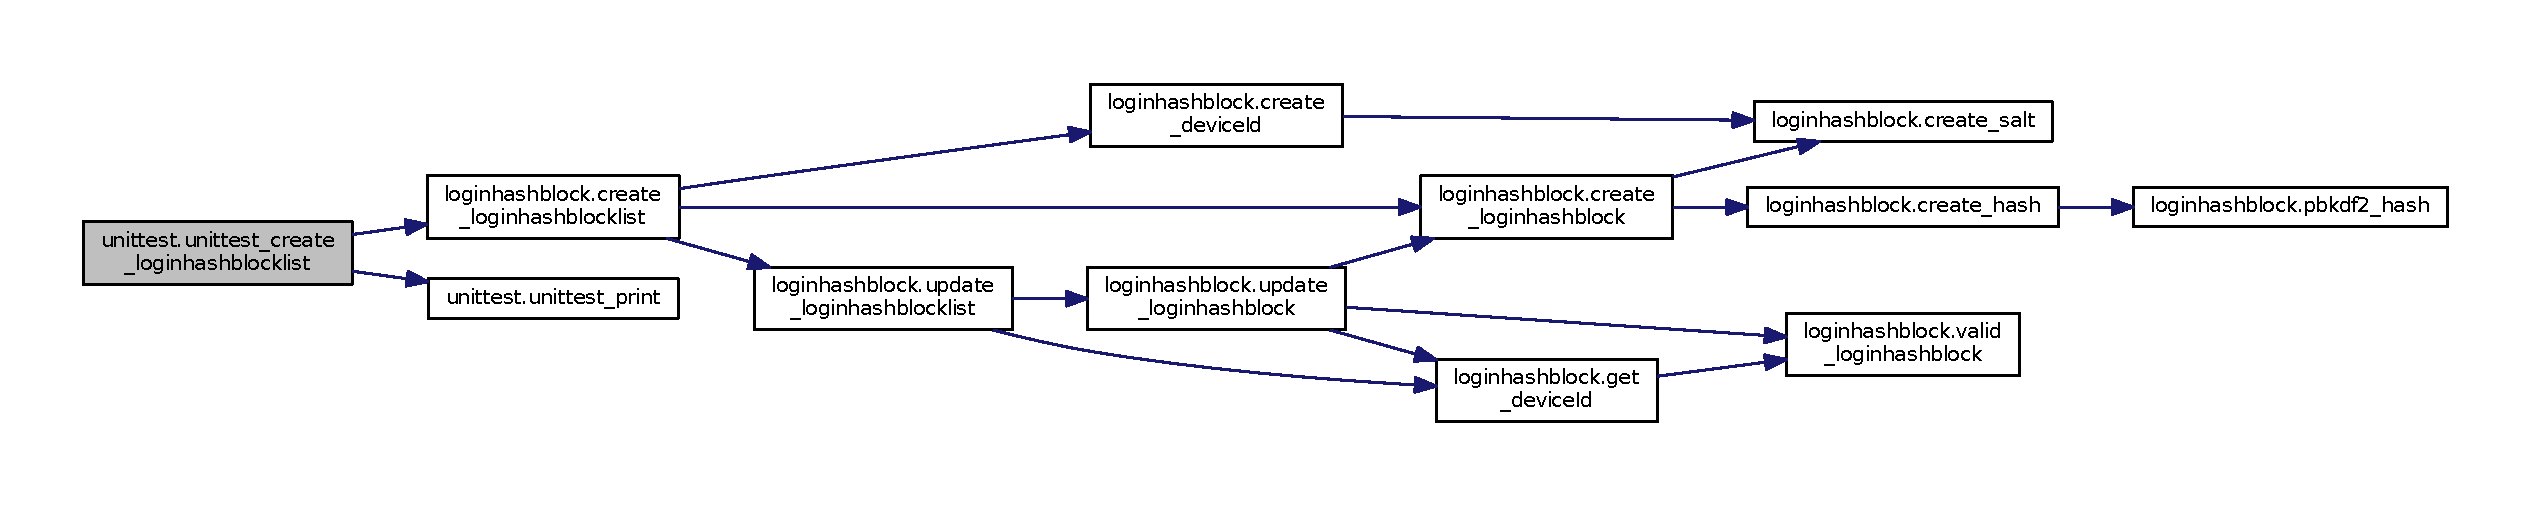
\includegraphics[width=350pt]{namespaceunittest_a0e10bea14aac2cc6a08d76f422b9328d_cgraph}
\end{center}
\end{figure}


\index{unittest@{unittest}!unittest\+\_\+print@{unittest\+\_\+print}}
\index{unittest\+\_\+print@{unittest\+\_\+print}!unittest@{unittest}}
\subsubsection[{\texorpdfstring{unittest\+\_\+print(message)}{unittest_print(message)}}]{\setlength{\rightskip}{0pt plus 5cm}def unittest.\+unittest\+\_\+print (
\begin{DoxyParamCaption}
\item[{}]{message}
\end{DoxyParamCaption}
)}\hypertarget{namespaceunittest_a217a1a3af5bc9748f2f6194bf79402bc}{}\label{namespaceunittest_a217a1a3af5bc9748f2f6194bf79402bc}


Definition at line 14 of file unittest.\+py.


\begin{DoxyCode}
14 \textcolor{keyword}{def }\hyperlink{namespaceunittest_a217a1a3af5bc9748f2f6194bf79402bc}{unittest\_print}(message):
15     print(bcolors.WARNING + message + bcolors.ENDC)
16 
\end{DoxyCode}


Here is the caller graph for this function\+:
\nopagebreak
\begin{figure}[H]
\begin{center}
\leavevmode
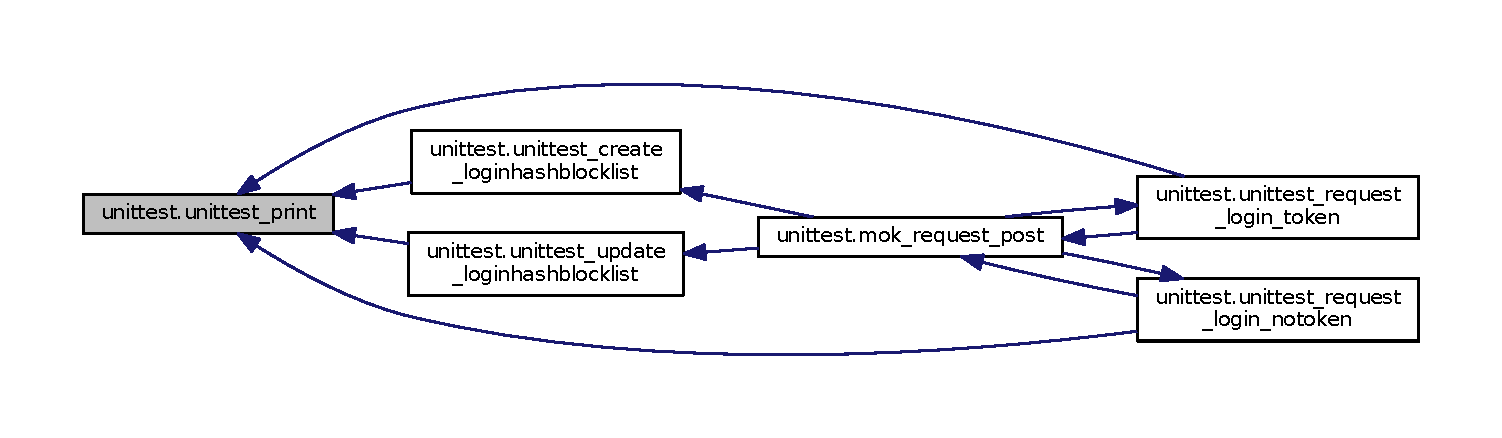
\includegraphics[width=350pt]{namespaceunittest_a217a1a3af5bc9748f2f6194bf79402bc_icgraph}
\end{center}
\end{figure}


\index{unittest@{unittest}!unittest\+\_\+title\+\_\+print@{unittest\+\_\+title\+\_\+print}}
\index{unittest\+\_\+title\+\_\+print@{unittest\+\_\+title\+\_\+print}!unittest@{unittest}}
\subsubsection[{\texorpdfstring{unittest\+\_\+title\+\_\+print(message)}{unittest_title_print(message)}}]{\setlength{\rightskip}{0pt plus 5cm}def unittest.\+unittest\+\_\+title\+\_\+print (
\begin{DoxyParamCaption}
\item[{}]{message}
\end{DoxyParamCaption}
)}\hypertarget{namespaceunittest_a642ec5401fe406315f1489d237ba826e}{}\label{namespaceunittest_a642ec5401fe406315f1489d237ba826e}


Definition at line 17 of file unittest.\+py.


\begin{DoxyCode}
17 \textcolor{keyword}{def }\hyperlink{namespaceunittest_a642ec5401fe406315f1489d237ba826e}{unittest\_title\_print}(message):
18     print(bcolors.OKGREEN + message + bcolors.ENDC)
19 
\end{DoxyCode}


Here is the caller graph for this function\+:
\nopagebreak
\begin{figure}[H]
\begin{center}
\leavevmode
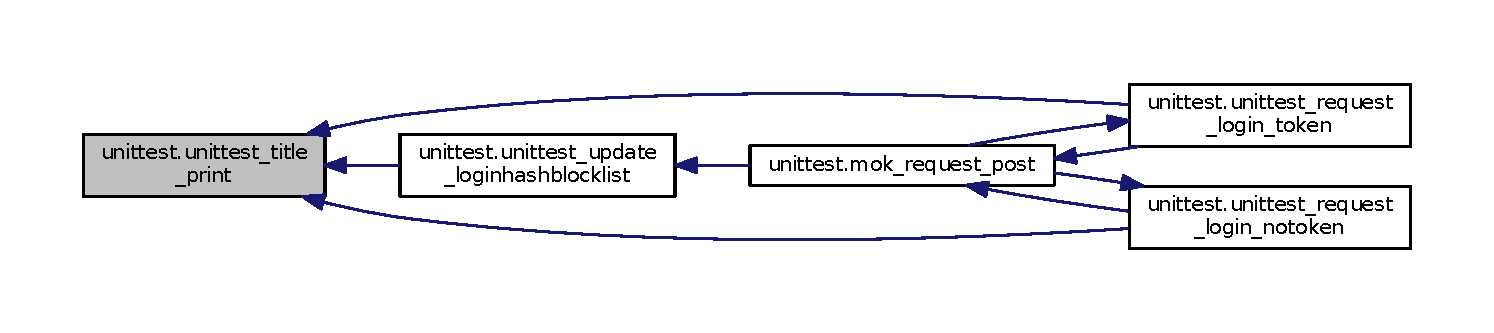
\includegraphics[width=350pt]{namespaceunittest_a642ec5401fe406315f1489d237ba826e_icgraph}
\end{center}
\end{figure}


\index{unittest@{unittest}!unittest\+\_\+update\+\_\+loginhashblocklist@{unittest\+\_\+update\+\_\+loginhashblocklist}}
\index{unittest\+\_\+update\+\_\+loginhashblocklist@{unittest\+\_\+update\+\_\+loginhashblocklist}!unittest@{unittest}}
\subsubsection[{\texorpdfstring{unittest\+\_\+update\+\_\+loginhashblocklist()}{unittest_update_loginhashblocklist()}}]{\setlength{\rightskip}{0pt plus 5cm}def unittest.\+unittest\+\_\+update\+\_\+loginhashblocklist (
\begin{DoxyParamCaption}
{}
\end{DoxyParamCaption}
)}\hypertarget{namespaceunittest_a9e16eaba67b93461be6ea8ef6332507a}{}\label{namespaceunittest_a9e16eaba67b93461be6ea8ef6332507a}


Definition at line 20 of file unittest.\+py.


\begin{DoxyCode}
20 \textcolor{keyword}{def }\hyperlink{namespaceunittest_a9e16eaba67b93461be6ea8ef6332507a}{unittest\_update\_loginhashblocklist}():
21     \textcolor{comment}{# case 01}
22     prev\_LHB = \textcolor{stringliteral}{'aCIXQRZ1$2b76784270f608bedf2757113041a6f6e81ab55faf787afde4e57e4376d302a1'}
23     LHBlistStr = \textcolor{stringliteral}{''}
24 
25     NewLHBlistStr = \hyperlink{namespaceloginhashblock_a7baa4021b9f57044f8227c2e0320ee2b}{update\_loginhashblocklist}(LHBlistStr, prev\_LHB, DEBUG=DEBUG)
26 
27     source = prev\_LHB.split(\textcolor{stringliteral}{'$'})
28     target = NewLHBlistStr.split(\textcolor{stringliteral}{'$'})
29 
30     \hyperlink{namespaceunittest_a642ec5401fe406315f1489d237ba826e}{unittest\_title\_print}(\textcolor{stringliteral}{"LHB is one, LHBlist is null"})
31     \textcolor{keywordflow}{if} source[0] == target[0] \textcolor{keywordflow}{and} source[1] != target[1]:
32         \hyperlink{namespaceunittest_a217a1a3af5bc9748f2f6194bf79402bc}{unittest\_print}(\textcolor{stringliteral}{"TestCase-01: Success"})
33     \textcolor{keywordflow}{else}:
34         \hyperlink{namespaceunittest_a217a1a3af5bc9748f2f6194bf79402bc}{unittest\_print}(\textcolor{stringliteral}{"TestCase-01: Fail"})
35 
36     \textcolor{comment}{# case 02}
37     LHBlistStr = \textcolor{stringliteral}{'
      aCIXQRZ1$2b76784270f608bedf2757113041a6f6e81ab55faf787afde4e57e4376d302a2,aCIXQRZ2$2b76784270f608bedf2757113041a6f6e81ab55faf787afde4e57e4376d302a3'}
38 
39     LHBlist = LHBlistStr.split(\textcolor{stringliteral}{','})
40     NewLHBlistStr = \hyperlink{namespaceloginhashblock_a7baa4021b9f57044f8227c2e0320ee2b}{update\_loginhashblocklist}(LHBlistStr, prev\_LHB, DEBUG=DEBUG)
41     targetList = NewLHBlistStr.split(\textcolor{stringliteral}{','})
42     target = targetList[0].split(\textcolor{stringliteral}{'$'})
43 
44     \hyperlink{namespaceunittest_a642ec5401fe406315f1489d237ba826e}{unittest\_title\_print}(\textcolor{stringliteral}{"LHB is one, LHBlist is two"})
45     \textcolor{keywordflow}{if} source[0] == target[0] \textcolor{keywordflow}{and} source[1] != target[1] \textcolor{keywordflow}{and} LHBlist[1] == targetList[1]:
46         \hyperlink{namespaceunittest_a217a1a3af5bc9748f2f6194bf79402bc}{unittest\_print}(\textcolor{stringliteral}{"TestCase-01: Success"})
47     \textcolor{keywordflow}{else}:
48         \hyperlink{namespaceunittest_a217a1a3af5bc9748f2f6194bf79402bc}{unittest\_print}(\textcolor{stringliteral}{"TestCase-01: Fail"})
49 
50     \textcolor{keywordflow}{if} LHBlistStr != NewLHBlistStr:
51         \hyperlink{namespaceunittest_a217a1a3af5bc9748f2f6194bf79402bc}{unittest\_print}(\textcolor{stringliteral}{"TestCase-02: Success"})
52     \textcolor{keywordflow}{else}:
53         \hyperlink{namespaceunittest_a217a1a3af5bc9748f2f6194bf79402bc}{unittest\_print}(\textcolor{stringliteral}{"TestCase-02: Fail"})
54 
55     \textcolor{comment}{# case 03}
56     LHBlistStr = \textcolor{stringliteral}{'aCIXQRZ3$2b76784270f608bedf2757113041a6f6e81ab55faf787afde4e57e4376d302a2'}
57 
58     LHBlist = LHBlistStr.split(\textcolor{stringliteral}{','})
59     NewLHBlistStr = \hyperlink{namespaceloginhashblock_a7baa4021b9f57044f8227c2e0320ee2b}{update\_loginhashblocklist}(LHBlistStr, prev\_LHB, DEBUG=DEBUG)
60     targetList = NewLHBlistStr.split(\textcolor{stringliteral}{','})
61     target = targetList[1].split(\textcolor{stringliteral}{'$'})
62 
63     \hyperlink{namespaceunittest_a642ec5401fe406315f1489d237ba826e}{unittest\_title\_print}(\textcolor{stringliteral}{"LHB is one, LHBlist is one, but devid is different so LHBlist
       will be updated LHB"})
64     \textcolor{keywordflow}{if} source[0] == target[0] \textcolor{keywordflow}{and} source[1] != target[1]:
65         \hyperlink{namespaceunittest_a217a1a3af5bc9748f2f6194bf79402bc}{unittest\_print}(\textcolor{stringliteral}{"TestCase-01: Success"})
66     \textcolor{keywordflow}{else}:
67         \hyperlink{namespaceunittest_a217a1a3af5bc9748f2f6194bf79402bc}{unittest\_print}(\textcolor{stringliteral}{"TestCase-01: Fail"})
68 
69     \textcolor{keywordflow}{if} LHBlistStr != NewLHBlistStr:
70         \hyperlink{namespaceunittest_a217a1a3af5bc9748f2f6194bf79402bc}{unittest\_print}(\textcolor{stringliteral}{"TestCase-02: Success"})
71     \textcolor{keywordflow}{else}:
72         \hyperlink{namespaceunittest_a217a1a3af5bc9748f2f6194bf79402bc}{unittest\_print}(\textcolor{stringliteral}{"TestCase-02: Fail"})
73 
74     \textcolor{keywordflow}{if} len(targetList) == 2:
75         \hyperlink{namespaceunittest_a217a1a3af5bc9748f2f6194bf79402bc}{unittest\_print}(\textcolor{stringliteral}{"TestCase-03: Success"})
76     \textcolor{keywordflow}{else}:
77         \hyperlink{namespaceunittest_a217a1a3af5bc9748f2f6194bf79402bc}{unittest\_print}(\textcolor{stringliteral}{"TestCase-03: Fail"})
78 
79     \textcolor{comment}{# case 04}
80     prev\_LHB = \textcolor{stringliteral}{''}
81     LHBlistStr = \textcolor{stringliteral}{'aCIXQRZ3$2b76784270f608bedf2757113041a6f6e81ab55faf787afde4e57e4376d302a2'}
82 
83     LHBlist = LHBlistStr.split(\textcolor{stringliteral}{','})
84     NewLHBlistStr = \hyperlink{namespaceloginhashblock_a7baa4021b9f57044f8227c2e0320ee2b}{update\_loginhashblocklist}(LHBlistStr, prev\_LHB, DEBUG=DEBUG)
85     targetList = NewLHBlistStr.split(\textcolor{stringliteral}{','})
86 
87     \hyperlink{namespaceunittest_a642ec5401fe406315f1489d237ba826e}{unittest\_title\_print}(\textcolor{stringliteral}{"LHB is null, LHBlist is one, su LHBlist will be maintained"})
88     \textcolor{keywordflow}{if} LHBlistStr == NewLHBlistStr:
89         \hyperlink{namespaceunittest_a217a1a3af5bc9748f2f6194bf79402bc}{unittest\_print}(\textcolor{stringliteral}{"TestCase-01: Success"})
90     \textcolor{keywordflow}{else}:
91         \hyperlink{namespaceunittest_a217a1a3af5bc9748f2f6194bf79402bc}{unittest\_print}(\textcolor{stringliteral}{"TestCase-01: Fail"})
92 
93     \textcolor{keywordflow}{if} len(targetList) == 1:
94         \hyperlink{namespaceunittest_a217a1a3af5bc9748f2f6194bf79402bc}{unittest\_print}(\textcolor{stringliteral}{"TestCase-02: Success"})
95     \textcolor{keywordflow}{else}:
96         \hyperlink{namespaceunittest_a217a1a3af5bc9748f2f6194bf79402bc}{unittest\_print}(\textcolor{stringliteral}{"TestCase-02: Fail"})
97 
\end{DoxyCode}


Here is the call graph for this function\+:\nopagebreak
\begin{figure}[H]
\begin{center}
\leavevmode
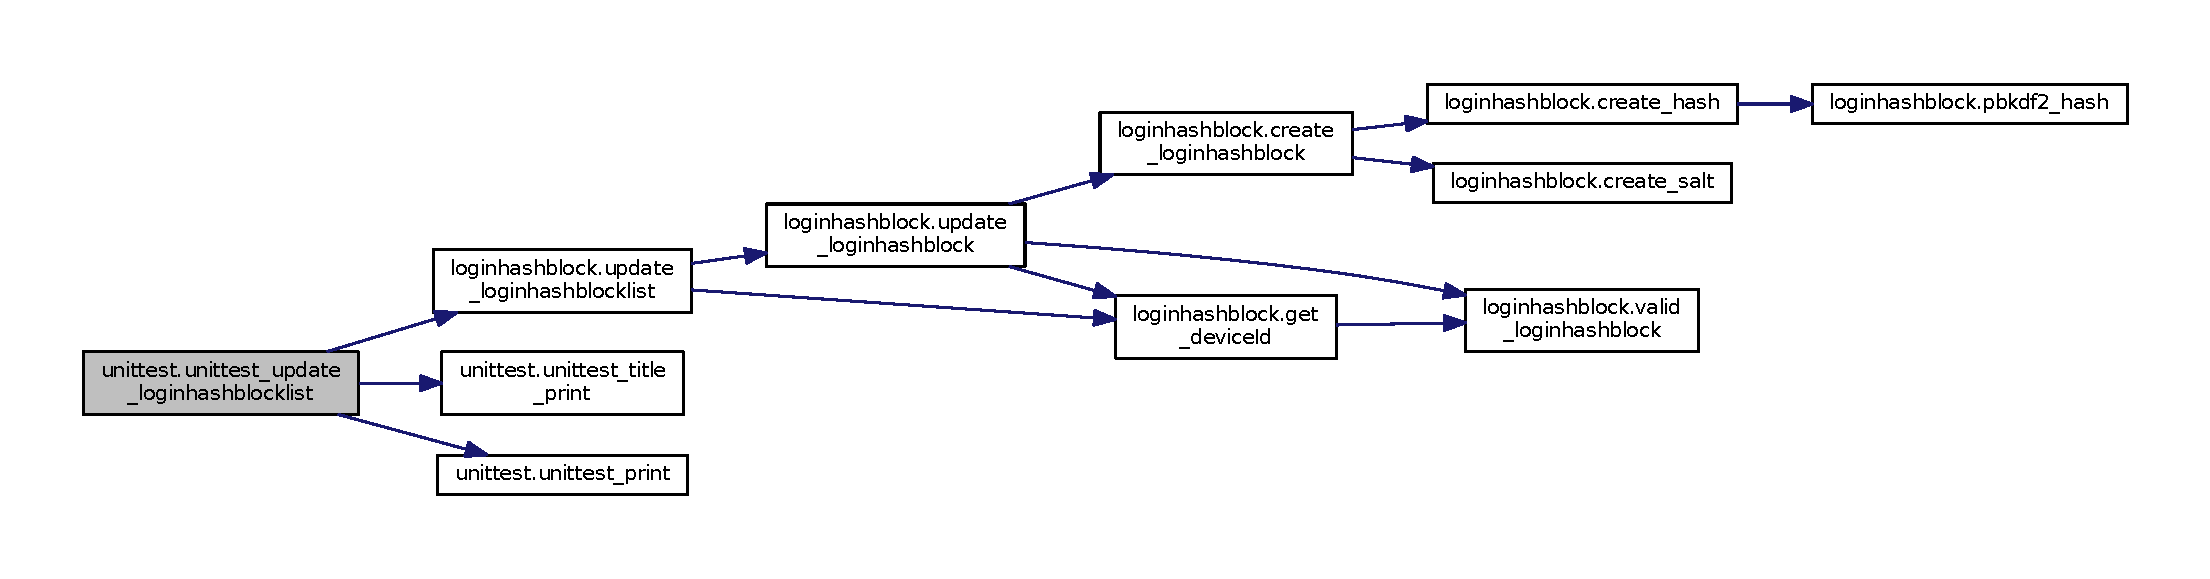
\includegraphics[width=350pt]{namespaceunittest_a9e16eaba67b93461be6ea8ef6332507a_cgraph}
\end{center}
\end{figure}




Here is the caller graph for this function\+:
\nopagebreak
\begin{figure}[H]
\begin{center}
\leavevmode
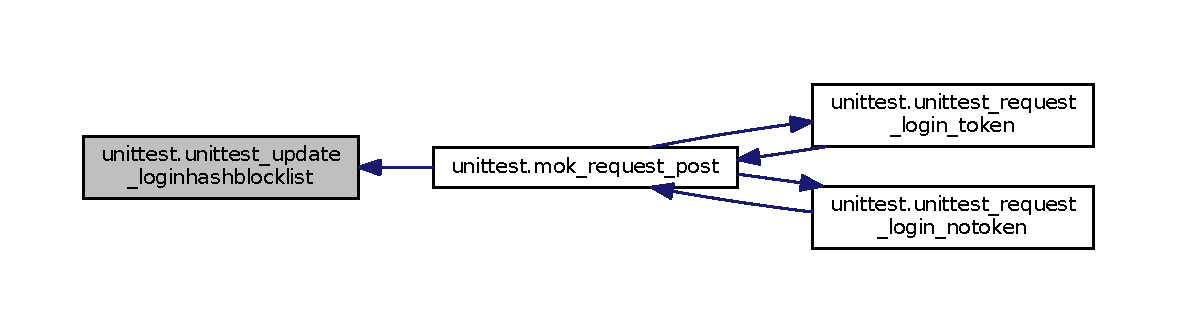
\includegraphics[width=350pt]{namespaceunittest_a9e16eaba67b93461be6ea8ef6332507a_icgraph}
\end{center}
\end{figure}




\subsection{Variable Documentation}
\index{unittest@{unittest}!D\+E\+B\+UG@{D\+E\+B\+UG}}
\index{D\+E\+B\+UG@{D\+E\+B\+UG}!unittest@{unittest}}
\subsubsection[{\texorpdfstring{D\+E\+B\+UG}{DEBUG}}]{\setlength{\rightskip}{0pt plus 5cm}bool unittest.\+D\+E\+B\+UG = False}\hypertarget{namespaceunittest_a6f95c254ae4668ea73efe6cf7ca3c36d}{}\label{namespaceunittest_a6f95c254ae4668ea73efe6cf7ca3c36d}


Definition at line 12 of file unittest.\+py.


\chapter{Class Documentation}
\hypertarget{classunittest_1_1bcolors}{}\doxysection{unittest.\+bcolors Class Reference}
\label{classunittest_1_1bcolors}\index{unittest.bcolors@{unittest.bcolors}}
\doxysubsection*{Static Public Attributes}
\begin{DoxyCompactItemize}
\item 
string \mbox{\hyperlink{classunittest_1_1bcolors_a0e8ae760e5f682550fc0b4e5638c47d0}{H\+E\+A\+D\+ER}} = \textquotesingle{}\textbackslash{}033\mbox{[}95m\textquotesingle{}
\item 
string \mbox{\hyperlink{classunittest_1_1bcolors_ac76b755140eefd1ff1eda35552b9ea01}{O\+K\+B\+L\+UE}} = \textquotesingle{}\textbackslash{}033\mbox{[}94m\textquotesingle{}
\item 
string \mbox{\hyperlink{classunittest_1_1bcolors_a4ea0a9b856e4906b0423ae6ae4ac16c8}{O\+K\+G\+R\+E\+EN}} = \textquotesingle{}\textbackslash{}033\mbox{[}92m\textquotesingle{}
\item 
string \mbox{\hyperlink{classunittest_1_1bcolors_acc0c1f9b572e877f80e4017094d3de68}{W\+A\+R\+N\+I\+NG}} = \textquotesingle{}\textbackslash{}033\mbox{[}93m\textquotesingle{}
\item 
string \mbox{\hyperlink{classunittest_1_1bcolors_a2dada3141c1e833e5a3cacd4f39dcf47}{F\+A\+IL}} = \textquotesingle{}\textbackslash{}033\mbox{[}91m\textquotesingle{}
\item 
string \mbox{\hyperlink{classunittest_1_1bcolors_a5db993c726eedb06b4a7efab09551f4e}{E\+N\+DC}} = \textquotesingle{}\textbackslash{}033\mbox{[}0m\textquotesingle{}
\item 
string \mbox{\hyperlink{classunittest_1_1bcolors_a95b491580216e848b313b0918ccea7ea}{B\+O\+LD}} = \textquotesingle{}\textbackslash{}033\mbox{[}1m\textquotesingle{}
\item 
string \mbox{\hyperlink{classunittest_1_1bcolors_ac181b1324b4847e254b738c74ef5fc00}{U\+N\+D\+E\+R\+L\+I\+NE}} = \textquotesingle{}\textbackslash{}033\mbox{[}4m\textquotesingle{}
\end{DoxyCompactItemize}


\doxysubsection{Detailed Description}


Definition at line 2 of file unittest.\+py.



\doxysubsection{Member Data Documentation}
\mbox{\Hypertarget{classunittest_1_1bcolors_a95b491580216e848b313b0918ccea7ea}\label{classunittest_1_1bcolors_a95b491580216e848b313b0918ccea7ea}} 
\index{unittest.bcolors@{unittest.bcolors}!BOLD@{BOLD}}
\index{BOLD@{BOLD}!unittest.bcolors@{unittest.bcolors}}
\doxysubsubsection{\texorpdfstring{BOLD}{BOLD}}
{\footnotesize\ttfamily string unittest.\+bcolors.\+B\+O\+LD = \textquotesingle{}\textbackslash{}033\mbox{[}1m\textquotesingle{}\hspace{0.3cm}{\ttfamily [static]}}



Definition at line 9 of file unittest.\+py.

\mbox{\Hypertarget{classunittest_1_1bcolors_a5db993c726eedb06b4a7efab09551f4e}\label{classunittest_1_1bcolors_a5db993c726eedb06b4a7efab09551f4e}} 
\index{unittest.bcolors@{unittest.bcolors}!ENDC@{ENDC}}
\index{ENDC@{ENDC}!unittest.bcolors@{unittest.bcolors}}
\doxysubsubsection{\texorpdfstring{ENDC}{ENDC}}
{\footnotesize\ttfamily string unittest.\+bcolors.\+E\+N\+DC = \textquotesingle{}\textbackslash{}033\mbox{[}0m\textquotesingle{}\hspace{0.3cm}{\ttfamily [static]}}



Definition at line 8 of file unittest.\+py.

\mbox{\Hypertarget{classunittest_1_1bcolors_a2dada3141c1e833e5a3cacd4f39dcf47}\label{classunittest_1_1bcolors_a2dada3141c1e833e5a3cacd4f39dcf47}} 
\index{unittest.bcolors@{unittest.bcolors}!FAIL@{FAIL}}
\index{FAIL@{FAIL}!unittest.bcolors@{unittest.bcolors}}
\doxysubsubsection{\texorpdfstring{FAIL}{FAIL}}
{\footnotesize\ttfamily string unittest.\+bcolors.\+F\+A\+IL = \textquotesingle{}\textbackslash{}033\mbox{[}91m\textquotesingle{}\hspace{0.3cm}{\ttfamily [static]}}



Definition at line 7 of file unittest.\+py.

\mbox{\Hypertarget{classunittest_1_1bcolors_a0e8ae760e5f682550fc0b4e5638c47d0}\label{classunittest_1_1bcolors_a0e8ae760e5f682550fc0b4e5638c47d0}} 
\index{unittest.bcolors@{unittest.bcolors}!HEADER@{HEADER}}
\index{HEADER@{HEADER}!unittest.bcolors@{unittest.bcolors}}
\doxysubsubsection{\texorpdfstring{HEADER}{HEADER}}
{\footnotesize\ttfamily string unittest.\+bcolors.\+H\+E\+A\+D\+ER = \textquotesingle{}\textbackslash{}033\mbox{[}95m\textquotesingle{}\hspace{0.3cm}{\ttfamily [static]}}



Definition at line 3 of file unittest.\+py.

\mbox{\Hypertarget{classunittest_1_1bcolors_ac76b755140eefd1ff1eda35552b9ea01}\label{classunittest_1_1bcolors_ac76b755140eefd1ff1eda35552b9ea01}} 
\index{unittest.bcolors@{unittest.bcolors}!OKBLUE@{OKBLUE}}
\index{OKBLUE@{OKBLUE}!unittest.bcolors@{unittest.bcolors}}
\doxysubsubsection{\texorpdfstring{OKBLUE}{OKBLUE}}
{\footnotesize\ttfamily string unittest.\+bcolors.\+O\+K\+B\+L\+UE = \textquotesingle{}\textbackslash{}033\mbox{[}94m\textquotesingle{}\hspace{0.3cm}{\ttfamily [static]}}



Definition at line 4 of file unittest.\+py.

\mbox{\Hypertarget{classunittest_1_1bcolors_a4ea0a9b856e4906b0423ae6ae4ac16c8}\label{classunittest_1_1bcolors_a4ea0a9b856e4906b0423ae6ae4ac16c8}} 
\index{unittest.bcolors@{unittest.bcolors}!OKGREEN@{OKGREEN}}
\index{OKGREEN@{OKGREEN}!unittest.bcolors@{unittest.bcolors}}
\doxysubsubsection{\texorpdfstring{OKGREEN}{OKGREEN}}
{\footnotesize\ttfamily string unittest.\+bcolors.\+O\+K\+G\+R\+E\+EN = \textquotesingle{}\textbackslash{}033\mbox{[}92m\textquotesingle{}\hspace{0.3cm}{\ttfamily [static]}}



Definition at line 5 of file unittest.\+py.

\mbox{\Hypertarget{classunittest_1_1bcolors_ac181b1324b4847e254b738c74ef5fc00}\label{classunittest_1_1bcolors_ac181b1324b4847e254b738c74ef5fc00}} 
\index{unittest.bcolors@{unittest.bcolors}!UNDERLINE@{UNDERLINE}}
\index{UNDERLINE@{UNDERLINE}!unittest.bcolors@{unittest.bcolors}}
\doxysubsubsection{\texorpdfstring{UNDERLINE}{UNDERLINE}}
{\footnotesize\ttfamily string unittest.\+bcolors.\+U\+N\+D\+E\+R\+L\+I\+NE = \textquotesingle{}\textbackslash{}033\mbox{[}4m\textquotesingle{}\hspace{0.3cm}{\ttfamily [static]}}



Definition at line 10 of file unittest.\+py.

\mbox{\Hypertarget{classunittest_1_1bcolors_acc0c1f9b572e877f80e4017094d3de68}\label{classunittest_1_1bcolors_acc0c1f9b572e877f80e4017094d3de68}} 
\index{unittest.bcolors@{unittest.bcolors}!WARNING@{WARNING}}
\index{WARNING@{WARNING}!unittest.bcolors@{unittest.bcolors}}
\doxysubsubsection{\texorpdfstring{WARNING}{WARNING}}
{\footnotesize\ttfamily string unittest.\+bcolors.\+W\+A\+R\+N\+I\+NG = \textquotesingle{}\textbackslash{}033\mbox{[}93m\textquotesingle{}\hspace{0.3cm}{\ttfamily [static]}}



Definition at line 6 of file unittest.\+py.



The documentation for this class was generated from the following file\+:\begin{DoxyCompactItemize}
\item 
loginhashblock/\mbox{\hyperlink{unittest_8py}{unittest.\+py}}\end{DoxyCompactItemize}

\hypertarget{classmain_1_1command}{}\section{main.\+command Class Reference}
\label{classmain_1_1command}\index{main.\+command@{main.\+command}}


Inheritance diagram for main.\+command\+:\nopagebreak
\begin{figure}[H]
\begin{center}
\leavevmode
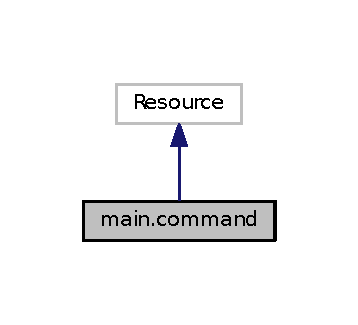
\includegraphics[width=172pt]{classmain_1_1command__inherit__graph}
\end{center}
\end{figure}


Collaboration diagram for main.\+command\+:\nopagebreak
\begin{figure}[H]
\begin{center}
\leavevmode
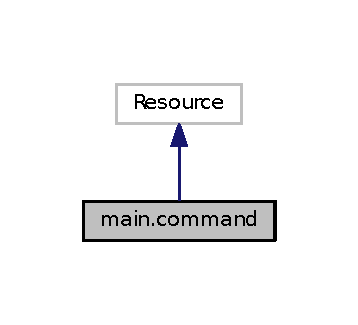
\includegraphics[width=172pt]{classmain_1_1command__coll__graph}
\end{center}
\end{figure}
\subsection*{Public Member Functions}
\begin{DoxyCompactItemize}
\item 
def \hyperlink{classmain_1_1command_a45d94d28b30ca81f482a4bca1bb3bc96}{get} (self)
\item 
def \hyperlink{classmain_1_1command_aad57d3ca75e00b96364b4dd9971f8d34}{post} (self)
\end{DoxyCompactItemize}


\subsection{Detailed Description}


Definition at line 274 of file main.\+py.



\subsection{Member Function Documentation}
\index{main\+::command@{main\+::command}!get@{get}}
\index{get@{get}!main\+::command@{main\+::command}}
\subsubsection[{\texorpdfstring{get(self)}{get(self)}}]{\setlength{\rightskip}{0pt plus 5cm}def main.\+command.\+get (
\begin{DoxyParamCaption}
\item[{}]{self}
\end{DoxyParamCaption}
)}\hypertarget{classmain_1_1command_a45d94d28b30ca81f482a4bca1bb3bc96}{}\label{classmain_1_1command_a45d94d28b30ca81f482a4bca1bb3bc96}


Definition at line 275 of file main.\+py.


\begin{DoxyCode}
275     \textcolor{keyword}{def }\hyperlink{classmain_1_1command_a45d94d28b30ca81f482a4bca1bb3bc96}{get}(self):
276         response = make\_response(render\_template(\textcolor{stringliteral}{'command.html'}))
277         \textcolor{keywordflow}{return} response
278 
\end{DoxyCode}
\index{main\+::command@{main\+::command}!post@{post}}
\index{post@{post}!main\+::command@{main\+::command}}
\subsubsection[{\texorpdfstring{post(self)}{post(self)}}]{\setlength{\rightskip}{0pt plus 5cm}def main.\+command.\+post (
\begin{DoxyParamCaption}
\item[{}]{self}
\end{DoxyParamCaption}
)}\hypertarget{classmain_1_1command_aad57d3ca75e00b96364b4dd9971f8d34}{}\label{classmain_1_1command_aad57d3ca75e00b96364b4dd9971f8d34}


Definition at line 279 of file main.\+py.


\begin{DoxyCode}
279     \textcolor{keyword}{def }\hyperlink{classmain_1_1command_aad57d3ca75e00b96364b4dd9971f8d34}{post}(self):
280         username = request.form.get(\textcolor{stringliteral}{'username'})
281         command = request.form.get(\textcolor{stringliteral}{'command'})
282         loginhashblock = request.form.get(\textcolor{stringliteral}{'loginhashblock'})
283         text = \textcolor{stringliteral}{"[info:command] username: \{\}, command: \{\}, loginhashblock: \{\}"}.format(username, command, 
      loginhashblock)
284         print(text)
285 
286         user = User.query.filter\_by(username=username).first()
287 
288         \textcolor{keywordflow}{if} \textcolor{keywordflow}{not} user:
289             resp = \{\textcolor{stringliteral}{'username'}:\textcolor{stringliteral}{'None'}, \textcolor{stringliteral}{'command'}:command, \textcolor{stringliteral}{'loginhashblock'}:\textcolor{stringliteral}{'None'}\}
290             \textcolor{keywordflow}{return} make\_response(resp, command)
291 
292         \textcolor{keywordflow}{if} command == str(3):
293             loginhashblock = user.Lhashblock
294 
295         \textcolor{keywordflow}{if} command == str(4):
296             user.Lhashblock = loginhashblock
297             db.session.commit()
298 
299         resp = \{\textcolor{stringliteral}{'username'}:username, \textcolor{stringliteral}{'command'}:command, \textcolor{stringliteral}{'loginhashblock'}:loginhashblock\}
300         \textcolor{keywordflow}{return} make\_response(resp, command)
301 
302 db.create\_all()
303 
304 api.add\_resource(index, \textcolor{stringliteral}{'/'})
305 api.add\_resource(logout, \textcolor{stringliteral}{'/logout'})
306 api.add\_resource(register, \textcolor{stringliteral}{'/register'})
307 api.add\_resource(twofactor, \textcolor{stringliteral}{'/twofactor'})
308 api.add\_resource(qrcode, \textcolor{stringliteral}{'/qrcode'})
309 api.add\_resource(login, \textcolor{stringliteral}{'/login'})
310 api.add\_resource(command, \textcolor{stringliteral}{'/command'})
311 
312 @app.errorhandler(404)
\end{DoxyCode}


The documentation for this class was generated from the following file\+:\begin{DoxyCompactItemize}
\item 
example/\hyperlink{main_8py}{main.\+py}\end{DoxyCompactItemize}

\hypertarget{classmain_1_1index}{}\doxysection{main.\+index Class Reference}
\label{classmain_1_1index}\index{main.index@{main.index}}


Inheritance diagram for main.\+index\+:\nopagebreak
\begin{figure}[H]
\begin{center}
\leavevmode
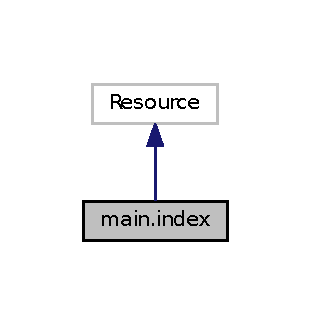
\includegraphics[width=144pt]{classmain_1_1index__inherit__graph}
\end{center}
\end{figure}


Collaboration diagram for main.\+index\+:\nopagebreak
\begin{figure}[H]
\begin{center}
\leavevmode
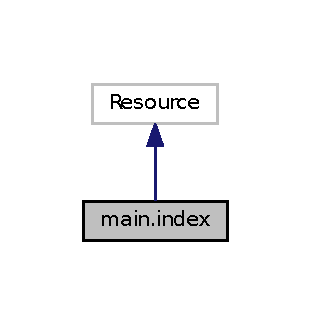
\includegraphics[width=144pt]{classmain_1_1index__coll__graph}
\end{center}
\end{figure}
\doxysubsection*{Public Member Functions}
\begin{DoxyCompactItemize}
\item 
def \mbox{\hyperlink{classmain_1_1index_aef2fa413e56c3ba4b7d0088148aa8ae8}{get}} (self)
\end{DoxyCompactItemize}


\doxysubsection{Detailed Description}


Definition at line 91 of file main.\+py.



\doxysubsection{Member Function Documentation}
\mbox{\Hypertarget{classmain_1_1index_aef2fa413e56c3ba4b7d0088148aa8ae8}\label{classmain_1_1index_aef2fa413e56c3ba4b7d0088148aa8ae8}} 
\index{main.index@{main.index}!get@{get}}
\index{get@{get}!main.index@{main.index}}
\doxysubsubsection{\texorpdfstring{get()}{get()}}
{\footnotesize\ttfamily def main.\+index.\+get (\begin{DoxyParamCaption}\item[{}]{self }\end{DoxyParamCaption})}



Definition at line 92 of file main.\+py.


\begin{DoxyCode}{0}
\DoxyCodeLine{92     \textcolor{keyword}{def }get(self):}
\DoxyCodeLine{93         response = make\_response(render\_template(\textcolor{stringliteral}{'index.html'}))}
\DoxyCodeLine{94         \textcolor{keywordflow}{return} response}
\DoxyCodeLine{95 }

\end{DoxyCode}


The documentation for this class was generated from the following file\+:\begin{DoxyCompactItemize}
\item 
example/\mbox{\hyperlink{main_8py}{main.\+py}}\end{DoxyCompactItemize}

\hypertarget{classmain_1_1login}{}\section{main.\+login Class Reference}
\label{classmain_1_1login}\index{main.\+login@{main.\+login}}


Inheritance diagram for main.\+login\+:\nopagebreak
\begin{figure}[H]
\begin{center}
\leavevmode
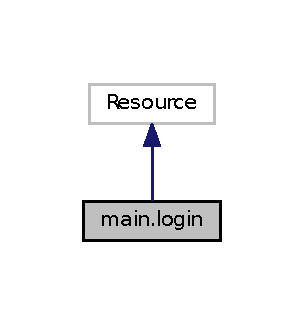
\includegraphics[width=146pt]{classmain_1_1login__inherit__graph}
\end{center}
\end{figure}


Collaboration diagram for main.\+login\+:\nopagebreak
\begin{figure}[H]
\begin{center}
\leavevmode
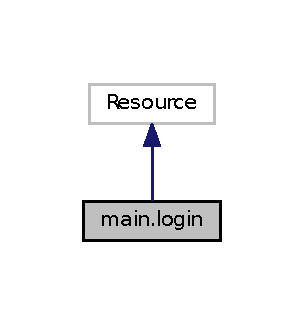
\includegraphics[width=146pt]{classmain_1_1login__coll__graph}
\end{center}
\end{figure}
\subsection*{Public Member Functions}
\begin{DoxyCompactItemize}
\item 
def \hyperlink{classmain_1_1login_a842b5fefc13556cbae749a8dc58d8e31}{get} (self)
\item 
def \hyperlink{classmain_1_1login_a71ff3f89aaf0f0c8502577445ab38744}{post} (self)
\end{DoxyCompactItemize}


\subsection{Detailed Description}


Definition at line 157 of file main.\+py.



\subsection{Member Function Documentation}
\index{main\+::login@{main\+::login}!get@{get}}
\index{get@{get}!main\+::login@{main\+::login}}
\subsubsection[{\texorpdfstring{get(self)}{get(self)}}]{\setlength{\rightskip}{0pt plus 5cm}def main.\+login.\+get (
\begin{DoxyParamCaption}
\item[{}]{self}
\end{DoxyParamCaption}
)}\hypertarget{classmain_1_1login_a842b5fefc13556cbae749a8dc58d8e31}{}\label{classmain_1_1login_a842b5fefc13556cbae749a8dc58d8e31}


Definition at line 158 of file main.\+py.


\begin{DoxyCode}
158     \textcolor{keyword}{def }\hyperlink{classmain_1_1login_a842b5fefc13556cbae749a8dc58d8e31}{get}(self):
159         \textcolor{keywordflow}{if} current\_user.is\_authenticated:
160             \textcolor{keywordflow}{return} redirect(url\_for(\textcolor{stringliteral}{'index'}))
161 
162         response = make\_response(render\_template(\textcolor{stringliteral}{'login.html'}))
163 
164         \textcolor{keywordflow}{return} response
165 
\end{DoxyCode}
\index{main\+::login@{main\+::login}!post@{post}}
\index{post@{post}!main\+::login@{main\+::login}}
\subsubsection[{\texorpdfstring{post(self)}{post(self)}}]{\setlength{\rightskip}{0pt plus 5cm}def main.\+login.\+post (
\begin{DoxyParamCaption}
\item[{}]{self}
\end{DoxyParamCaption}
)}\hypertarget{classmain_1_1login_a71ff3f89aaf0f0c8502577445ab38744}{}\label{classmain_1_1login_a71ff3f89aaf0f0c8502577445ab38744}


Definition at line 166 of file main.\+py.


\begin{DoxyCode}
166     \textcolor{keyword}{def }\hyperlink{classmain_1_1login_a71ff3f89aaf0f0c8502577445ab38744}{post}(self):
167         username = request.form.get(\textcolor{stringliteral}{'username'})
168         password = request.form.get(\textcolor{stringliteral}{'password'})
169         token = request.form.get(\textcolor{stringliteral}{'token'})
170         prev\_LHB = request.form.get(\textcolor{stringliteral}{'loginhashblock'})
171 
172         \textcolor{keywordflow}{if} \textcolor{keywordflow}{not} username:
173             flash(\textcolor{stringliteral}{'username is null'})
174             \textcolor{keywordflow}{return} make\_response(\textcolor{stringliteral}{'Error'}, 302)
175 
176         \textcolor{keywordflow}{if} \textcolor{keywordflow}{not} password:
177             flash(\textcolor{stringliteral}{'password is null'})
178             \textcolor{keywordflow}{return} make\_response(\textcolor{stringliteral}{'Error'}, 302)
179 
180         user = User.query.filter\_by(username=username).first()
181 
182         \textcolor{keywordflow}{if} \textcolor{keywordflow}{not} user:
183             flash(\textcolor{stringliteral}{'not registered username'})
184             \textcolor{keywordflow}{return} make\_response(\textcolor{stringliteral}{'Error'}, 302)
185 
186         \textcolor{keywordflow}{if} \textcolor{keywordflow}{not} user.verify\_password(password):
187             flash(\textcolor{stringliteral}{'password was wrong'})
188             \textcolor{keywordflow}{return} make\_response(\textcolor{stringliteral}{'Error'}, 302)
189 
190         \textcolor{keywordflow}{if} token:
191             \textcolor{keywordflow}{if} \textcolor{keywordflow}{not} user.verify\_totp(token):
192                 flash(\textcolor{stringliteral}{'OTP was wrong'})
193                 \textcolor{keywordflow}{return} make\_response(\textcolor{stringliteral}{'Error'}, 302)
194 
195             \textcolor{keywordflow}{if} prev\_LHB:
196                 \textcolor{keywordflow}{if} \textcolor{keywordflow}{not} \hyperlink{namespaceloginhashblock_adb424539d851426da7b65d53c5a6d577}{valid\_loginhashblock}(prev\_LHB):
197                     flash(\textcolor{stringliteral}{'Your account is suspected of being stolen. OTP is required.'})
198                     \textcolor{keywordflow}{return} make\_response(\textcolor{stringliteral}{'Error'}, 302)
199 
200                 LHBlistStr, new\_LHB = \hyperlink{namespaceloginhashblock_a2bcc7ddd0fcc3788572dd77808cb624d}{update\_loginhashblocklist}(user.Lhashblock, 
      prev\_LHB, DEBUG=DEBUG)
201             \textcolor{keywordflow}{else}:
202                 LHBlistStr, new\_LHB = \hyperlink{namespaceloginhashblock_a550707107141dfb228ca4294d7ea31b4}{create\_loginhashblocklist}(user.Lhashblock, 
      DEBUG=DEBUG)
203         \textcolor{keywordflow}{else}:
204             \textcolor{keywordflow}{if} \textcolor{keywordflow}{not} user.Lhashblock:
205                 flash(\textcolor{stringliteral}{'Your account is first login, OTP is required.'})
206                 \textcolor{keywordflow}{return} make\_response(\textcolor{stringliteral}{'Error'}, 302)
207 
208             \textcolor{keywordflow}{if} prev\_LHB:
209                 \textcolor{keywordflow}{if} \textcolor{keywordflow}{not} \hyperlink{namespaceloginhashblock_adb424539d851426da7b65d53c5a6d577}{valid\_loginhashblock}(prev\_LHB):
210                     flash(\textcolor{stringliteral}{'Your account is suspected of being stolen. OTP is required.'})
211                     print(\textcolor{stringliteral}{"Error valid\_loginhashblock"})
212                     \textcolor{keywordflow}{return} make\_response(\textcolor{stringliteral}{'Error'}, 302)
213 
214                 \textcolor{keywordflow}{if} \textcolor{keywordflow}{not} \hyperlink{namespaceloginhashblock_aa5bb94484a68d0bbebce23b4cfeeb4b7}{verify\_loginhashblock}(user.Lhashblock, prev\_LHB):
215                     flash(\textcolor{stringliteral}{'Your account is suspected of being stolen. OTP is required.'})
216                     print(\textcolor{stringliteral}{"Error verify\_loginhashblock"})
217                     \textcolor{keywordflow}{return} make\_response(\textcolor{stringliteral}{'Error'}, 302)
218 
219                 LHBlistStr, new\_LHB = \hyperlink{namespaceloginhashblock_a2bcc7ddd0fcc3788572dd77808cb624d}{update\_loginhashblocklist}(user.Lhashblock, 
      prev\_LHB, DEBUG=DEBUG)
220             \textcolor{keywordflow}{else}:
221                 flash(\textcolor{stringliteral}{'Error! Debug Mode'})
222                 \textcolor{keywordflow}{return} make\_response(\textcolor{stringliteral}{'Error'}, 302)
223 
224         user.Lhashblock = LHBlistStr
225         db.session.commit()
226 
227         \textcolor{keywordflow}{if} DEBUG:
228             text = \textcolor{stringliteral}{"[info:login:post]\(\backslash\)nprev\_hashblock[\{\}]: \{\}\(\backslash\)nnext\_hashblock[\{\}]: \{\}"}.format(username,
      prev\_LHB,username,new\_LHB)
229             print(text)
230 
231         login\_user(user)
232         flash(\textcolor{stringliteral}{'You are now logged in!'})
233         condition = \textcolor{keyword}{True}
234         response = make\_response(render\_template(\textcolor{stringliteral}{'index.html'}, condition=condition, username=username, 
      LoginHB=new\_LHB))
235         \textcolor{keywordflow}{return} response
236 
\end{DoxyCode}


Here is the call graph for this function\+:\nopagebreak
\begin{figure}[H]
\begin{center}
\leavevmode
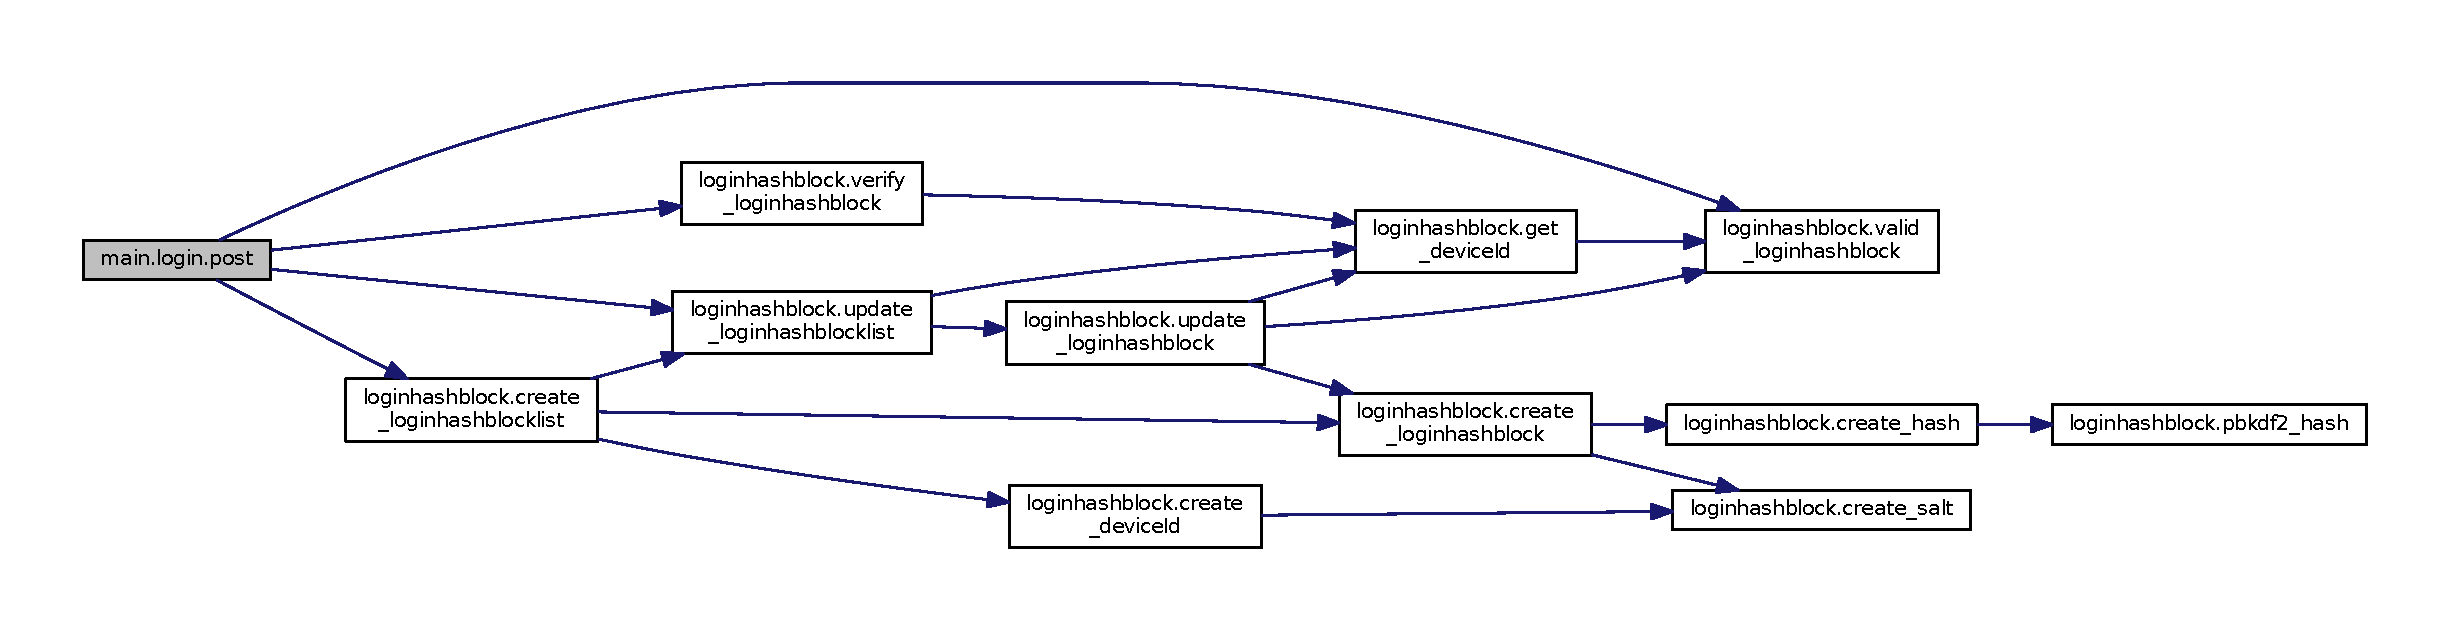
\includegraphics[width=350pt]{classmain_1_1login_a71ff3f89aaf0f0c8502577445ab38744_cgraph}
\end{center}
\end{figure}




The documentation for this class was generated from the following file\+:\begin{DoxyCompactItemize}
\item 
example/\hyperlink{main_8py}{main.\+py}\end{DoxyCompactItemize}

\hypertarget{classmain_1_1logout}{}\section{main.\+logout Class Reference}
\label{classmain_1_1logout}\index{main.\+logout@{main.\+logout}}


Inheritance diagram for main.\+logout\+:
\nopagebreak
\begin{figure}[H]
\begin{center}
\leavevmode
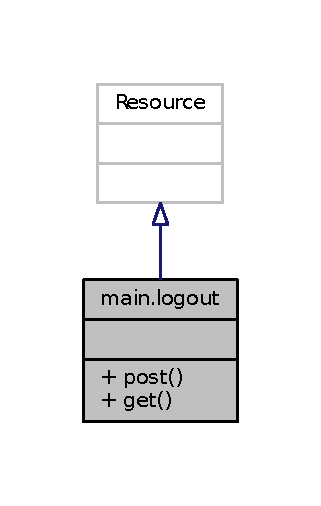
\includegraphics[width=154pt]{classmain_1_1logout__inherit__graph}
\end{center}
\end{figure}


Collaboration diagram for main.\+logout\+:
\nopagebreak
\begin{figure}[H]
\begin{center}
\leavevmode
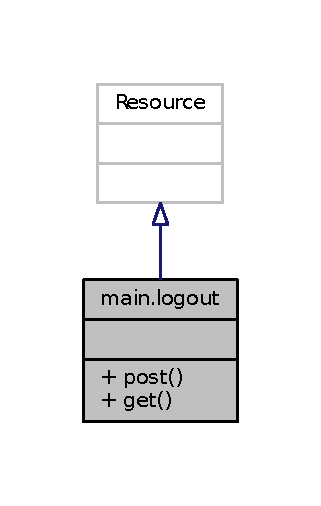
\includegraphics[width=154pt]{classmain_1_1logout__coll__graph}
\end{center}
\end{figure}
\subsection*{Public Member Functions}
\begin{DoxyCompactItemize}
\item 
def \hyperlink{classmain_1_1logout_a726ef779e6bf4da8974eae3209276922}{post} (self)
\item 
def \hyperlink{classmain_1_1logout_a014267caa3d9cc9e42fdb71ef54ce43b}{get} (self)
\end{DoxyCompactItemize}


\subsection{Detailed Description}


Definition at line 237 of file main.\+py.



\subsection{Member Function Documentation}
\index{main\+::logout@{main\+::logout}!get@{get}}
\index{get@{get}!main\+::logout@{main\+::logout}}
\subsubsection[{\texorpdfstring{get(self)}{get(self)}}]{\setlength{\rightskip}{0pt plus 5cm}def main.\+logout.\+get (
\begin{DoxyParamCaption}
\item[{}]{self}
\end{DoxyParamCaption}
)}\hypertarget{classmain_1_1logout_a014267caa3d9cc9e42fdb71ef54ce43b}{}\label{classmain_1_1logout_a014267caa3d9cc9e42fdb71ef54ce43b}


Definition at line 267 of file main.\+py.


\begin{DoxyCode}
267     \textcolor{keyword}{def }\hyperlink{classmain_1_1logout_a014267caa3d9cc9e42fdb71ef54ce43b}{get}(self):
268         \textcolor{keywordflow}{if} current\_user.is\_active == \textcolor{keyword}{False}:
269             \textcolor{keywordflow}{return} redirect(url\_for(\textcolor{stringliteral}{'index'}))
270 
271         response = make\_response(render\_template(\textcolor{stringliteral}{'logout.html'}))
272         \textcolor{keywordflow}{return} response
273 
\end{DoxyCode}
\index{main\+::logout@{main\+::logout}!post@{post}}
\index{post@{post}!main\+::logout@{main\+::logout}}
\subsubsection[{\texorpdfstring{post(self)}{post(self)}}]{\setlength{\rightskip}{0pt plus 5cm}def main.\+logout.\+post (
\begin{DoxyParamCaption}
\item[{}]{self}
\end{DoxyParamCaption}
)}\hypertarget{classmain_1_1logout_a726ef779e6bf4da8974eae3209276922}{}\label{classmain_1_1logout_a726ef779e6bf4da8974eae3209276922}


Definition at line 238 of file main.\+py.


\begin{DoxyCode}
238     \textcolor{keyword}{def }\hyperlink{classmain_1_1logout_a726ef779e6bf4da8974eae3209276922}{post}(self):
239         username = request.form.get(\textcolor{stringliteral}{'username'})
240         prev\_LHB = request.form.get(\textcolor{stringliteral}{'loginhashblock'})
241 
242         \textcolor{keywordflow}{if} current\_user.is\_active == \textcolor{keyword}{False}:
243             \textcolor{keywordflow}{return} redirect(url\_for(\textcolor{stringliteral}{'index'}))
244 
245         user = User.query.filter\_by(username=username).first()
246 
247         \textcolor{keywordflow}{if} DEBUG:
248             \hyperlink{namespaceloginhashblock_a1096aa8494b9c5875decc029d8b40ea9}{print\_LHBlist}(user.Lhashblock)
249 
250         \textcolor{keywordflow}{if} \textcolor{keywordflow}{not} prev\_LHB:
251             print(\textcolor{stringliteral}{"[info:logout:post] GO TO OTP"})
252         \textcolor{keywordflow}{else}:
253             LHBlistStr, new\_LHB = \hyperlink{namespaceloginhashblock_a2bcc7ddd0fcc3788572dd77808cb624d}{update\_loginhashblocklist}(user.Lhashblock, 
      prev\_LHB, DEBUG=DEBUG)
254             user.Lhashblock = LHBlistStr
255             db.session.commit()
256 
257         condition = \textcolor{keyword}{True}
258         logout\_user()
259 
260         \textcolor{keywordflow}{if} DEBUG:
261             text = \textcolor{stringliteral}{"[info:logout:post]\(\backslash\)nprev\_hashblock[\{\}]: \{\}\(\backslash\)nnext\_hashblock[\{\}]: \{\}"}.format(username,
      prev\_LHB,username,new\_LHB)
262             print(text)
263 
264         response = make\_response(render\_template(\textcolor{stringliteral}{'index.html'}, condition=condition, username=username, 
      LoginHB=new\_LHB))
265         \textcolor{keywordflow}{return} response
266 
\end{DoxyCode}


Here is the call graph for this function\+:
\nopagebreak
\begin{figure}[H]
\begin{center}
\leavevmode
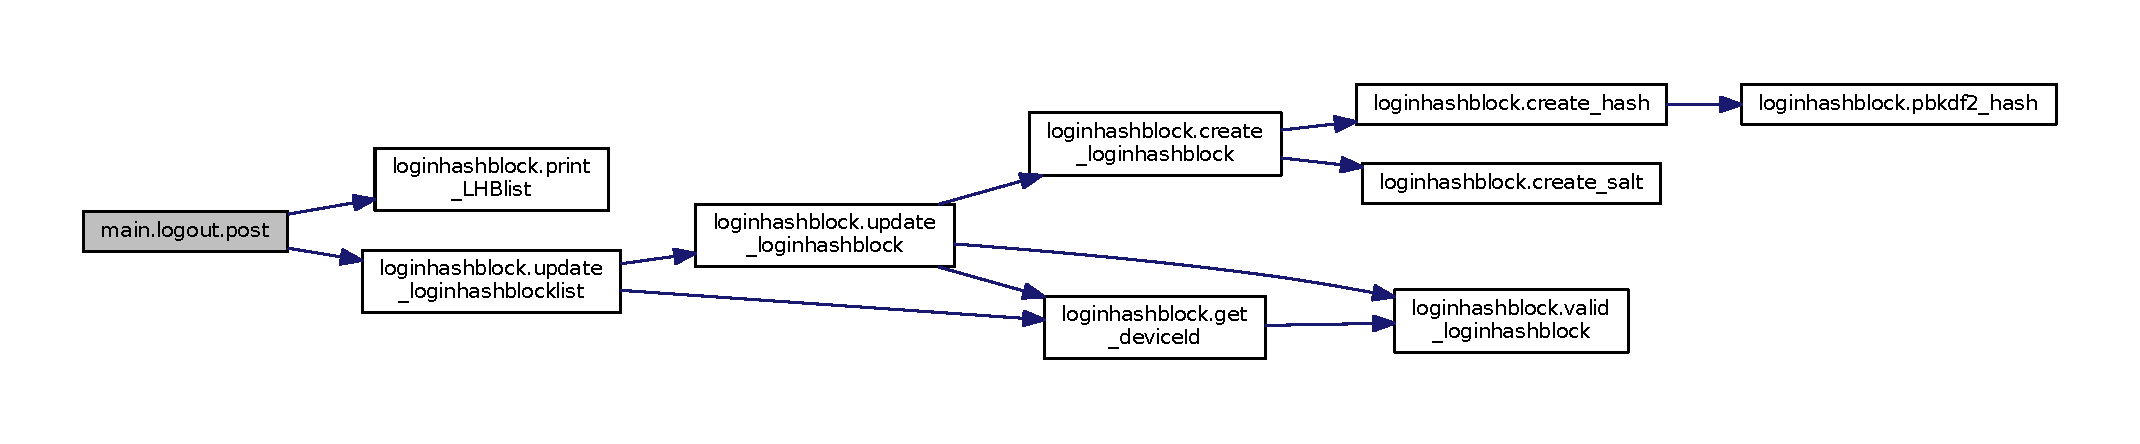
\includegraphics[width=350pt]{classmain_1_1logout_a726ef779e6bf4da8974eae3209276922_cgraph}
\end{center}
\end{figure}




The documentation for this class was generated from the following file\+:\begin{DoxyCompactItemize}
\item 
example/\hyperlink{main_8py}{main.\+py}\end{DoxyCompactItemize}

\hypertarget{classmain_1_1qrcode}{}\section{main.\+qrcode Class Reference}
\label{classmain_1_1qrcode}\index{main.\+qrcode@{main.\+qrcode}}


Inheritance diagram for main.\+qrcode\+:
\nopagebreak
\begin{figure}[H]
\begin{center}
\leavevmode
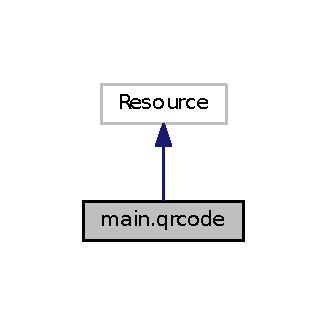
\includegraphics[width=157pt]{classmain_1_1qrcode__inherit__graph}
\end{center}
\end{figure}


Collaboration diagram for main.\+qrcode\+:
\nopagebreak
\begin{figure}[H]
\begin{center}
\leavevmode
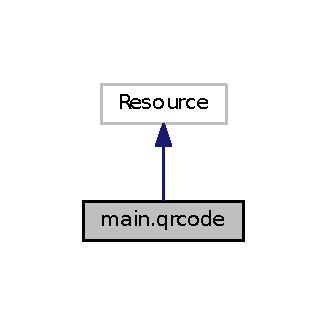
\includegraphics[width=157pt]{classmain_1_1qrcode__coll__graph}
\end{center}
\end{figure}
\subsection*{Public Member Functions}
\begin{DoxyCompactItemize}
\item 
def \hyperlink{classmain_1_1qrcode_af826915a83b6a4d5c91686b332662da3}{get} (self)
\end{DoxyCompactItemize}


\subsection{Detailed Description}


Definition at line 141 of file main.\+py.



\subsection{Member Function Documentation}
\index{main\+::qrcode@{main\+::qrcode}!get@{get}}
\index{get@{get}!main\+::qrcode@{main\+::qrcode}}
\subsubsection[{\texorpdfstring{get(self)}{get(self)}}]{\setlength{\rightskip}{0pt plus 5cm}def main.\+qrcode.\+get (
\begin{DoxyParamCaption}
\item[{}]{self}
\end{DoxyParamCaption}
)}\hypertarget{classmain_1_1qrcode_af826915a83b6a4d5c91686b332662da3}{}\label{classmain_1_1qrcode_af826915a83b6a4d5c91686b332662da3}


Definition at line 142 of file main.\+py.


\begin{DoxyCode}
142     \textcolor{keyword}{def }\hyperlink{classmain_1_1qrcode_af826915a83b6a4d5c91686b332662da3}{get}(self):
143         \textcolor{keywordflow}{if} \textcolor{stringliteral}{'username'} \textcolor{keywordflow}{not} \textcolor{keywordflow}{in} session:
144             abort(404)
145 
146         user = User.query.filter\_by(username=session[\textcolor{stringliteral}{'username'}]).first()
147 
148         \textcolor{keywordflow}{if} user \textcolor{keywordflow}{is} \textcolor{keywordtype}{None}:
149             abort(404)
150 
151         del session[\textcolor{stringliteral}{'username'}]
152 
153         url = pyqrcode.create(user.get\_totp\_uri())
154         stream = BytesIO()
155         url.svg(stream, scale=3)
156         param = \{\textcolor{stringliteral}{'Content-Type'}: \textcolor{stringliteral}{'image/svg+xml'}, \textcolor{stringliteral}{'Cache-Control'}: \textcolor{stringliteral}{'no-cache, no-store, must-revalidate'},\textcolor{stringliteral}{'
      Pragma'}: \textcolor{stringliteral}{'no-cache'}, \textcolor{stringliteral}{'Expires'}: \textcolor{stringliteral}{'0'}\}
157         response = make\_response(stream.getvalue(), 200, param)
158         \textcolor{keywordflow}{return} response
159 
\end{DoxyCode}


The documentation for this class was generated from the following file\+:\begin{DoxyCompactItemize}
\item 
example/\hyperlink{main_8py}{main.\+py}\end{DoxyCompactItemize}

\hypertarget{classmain_1_1register}{}\section{main.\+register Class Reference}
\label{classmain_1_1register}\index{main.\+register@{main.\+register}}


Inheritance diagram for main.\+register\+:\nopagebreak
\begin{figure}[H]
\begin{center}
\leavevmode
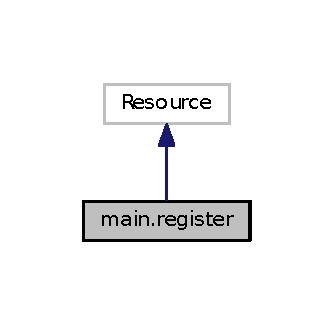
\includegraphics[width=160pt]{classmain_1_1register__inherit__graph}
\end{center}
\end{figure}


Collaboration diagram for main.\+register\+:\nopagebreak
\begin{figure}[H]
\begin{center}
\leavevmode
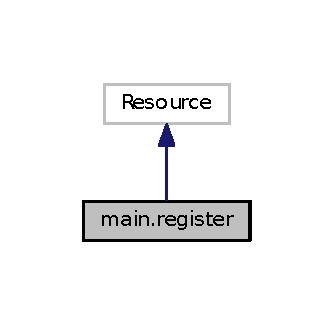
\includegraphics[width=160pt]{classmain_1_1register__coll__graph}
\end{center}
\end{figure}
\subsection*{Public Member Functions}
\begin{DoxyCompactItemize}
\item 
def \hyperlink{classmain_1_1register_a0bc316df389231c4741d9b2460b448f2}{get} (self)
\item 
def \hyperlink{classmain_1_1register_a890271e936f3717c3ac52428f7a058ef}{post} (self)
\end{DoxyCompactItemize}


\subsection{Detailed Description}


Definition at line 96 of file main.\+py.



\subsection{Member Function Documentation}
\index{main\+::register@{main\+::register}!get@{get}}
\index{get@{get}!main\+::register@{main\+::register}}
\subsubsection[{\texorpdfstring{get(self)}{get(self)}}]{\setlength{\rightskip}{0pt plus 5cm}def main.\+register.\+get (
\begin{DoxyParamCaption}
\item[{}]{self}
\end{DoxyParamCaption}
)}\hypertarget{classmain_1_1register_a0bc316df389231c4741d9b2460b448f2}{}\label{classmain_1_1register_a0bc316df389231c4741d9b2460b448f2}


Definition at line 97 of file main.\+py.


\begin{DoxyCode}
97     \textcolor{keyword}{def }\hyperlink{classmain_1_1register_a0bc316df389231c4741d9b2460b448f2}{get}(self):
98         \textcolor{keywordflow}{if} current\_user.is\_authenticated:
99             \textcolor{keywordflow}{return} redirect(url\_for(\textcolor{stringliteral}{'index'}))
100 
101         form = \hyperlink{classmain_1_1RegisterForm}{RegisterForm}()
102         response = make\_response(render\_template(\textcolor{stringliteral}{'register.html'}, form=form))
103         \textcolor{keywordflow}{return} response
104 
\end{DoxyCode}
\index{main\+::register@{main\+::register}!post@{post}}
\index{post@{post}!main\+::register@{main\+::register}}
\subsubsection[{\texorpdfstring{post(self)}{post(self)}}]{\setlength{\rightskip}{0pt plus 5cm}def main.\+register.\+post (
\begin{DoxyParamCaption}
\item[{}]{self}
\end{DoxyParamCaption}
)}\hypertarget{classmain_1_1register_a890271e936f3717c3ac52428f7a058ef}{}\label{classmain_1_1register_a890271e936f3717c3ac52428f7a058ef}


Definition at line 105 of file main.\+py.


\begin{DoxyCode}
105     \textcolor{keyword}{def }\hyperlink{classmain_1_1register_a890271e936f3717c3ac52428f7a058ef}{post}(self):
106         username = request.form.get(\textcolor{stringliteral}{'username'})
107         password = request.form.get(\textcolor{stringliteral}{'password'})
108         password\_again = request.form.get(\textcolor{stringliteral}{'password\_again'})
109 
110         user = User.query.filter\_by(username=username).first()
111 
112         \textcolor{keywordflow}{if} user \textcolor{keywordflow}{is} \textcolor{keywordflow}{not} \textcolor{keywordtype}{None}:
113             flash(\textcolor{stringliteral}{'Username already exists.'})
114             \textcolor{keywordflow}{return} redirect(url\_for(\textcolor{stringliteral}{'register'}))
115 
116         user = \hyperlink{classmain_1_1User}{User}(username=username, password=password)
117         db.session.add(user)
118         db.session.commit()
119 
120         session[\textcolor{stringliteral}{'username'}] = user.username
121 
122         \textcolor{keywordflow}{return} redirect(url\_for(\textcolor{stringliteral}{'twofactor'}))
123 
\end{DoxyCode}


The documentation for this class was generated from the following file\+:\begin{DoxyCompactItemize}
\item 
example/\hyperlink{main_8py}{main.\+py}\end{DoxyCompactItemize}

\hypertarget{classmain_1_1RegisterForm}{}\doxysection{main.\+Register\+Form Class Reference}
\label{classmain_1_1RegisterForm}\index{main.RegisterForm@{main.RegisterForm}}


Inheritance diagram for main.\+Register\+Form\+:\nopagebreak
\begin{figure}[H]
\begin{center}
\leavevmode
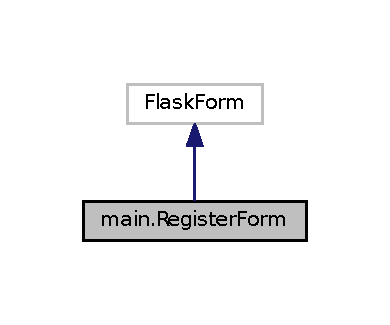
\includegraphics[width=181pt]{classmain_1_1RegisterForm__inherit__graph}
\end{center}
\end{figure}


Collaboration diagram for main.\+Register\+Form\+:\nopagebreak
\begin{figure}[H]
\begin{center}
\leavevmode
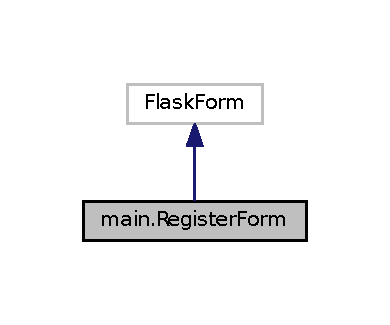
\includegraphics[width=181pt]{classmain_1_1RegisterForm__coll__graph}
\end{center}
\end{figure}
\doxysubsection*{Static Public Attributes}
\begin{DoxyCompactItemize}
\item 
\mbox{\hyperlink{classmain_1_1RegisterForm_a358e684fade440a73243b01b69778fe9}{username}} = String\+Field(\textquotesingle{}Username\textquotesingle{}, validators=\mbox{[}Required(), Length(1, 64)\mbox{]})
\item 
\mbox{\hyperlink{classmain_1_1RegisterForm_a995a1a67b85b4165619b8cb0863940f0}{password}} = Password\+Field(\textquotesingle{}Password\textquotesingle{}, validators=\mbox{[}Required()\mbox{]})
\item 
\mbox{\hyperlink{classmain_1_1RegisterForm_a045a58303acc98394aedb828655268ab}{password\+\_\+again}} = Password\+Field(\textquotesingle{}Password again\textquotesingle{}, validators=\mbox{[}Required(), Equal\+To(\textquotesingle{}\mbox{\hyperlink{classmain_1_1RegisterForm_a995a1a67b85b4165619b8cb0863940f0}{password}}\textquotesingle{})\mbox{]})
\item 
\mbox{\hyperlink{classmain_1_1RegisterForm_a1d788d2aac9c4ac25887eb8b2072d170}{submit}} = Submit\+Field(\textquotesingle{}Register\textquotesingle{})
\end{DoxyCompactItemize}


\doxysubsection{Detailed Description}
\begin{DoxyVerb}Registration form.\end{DoxyVerb}
 

Definition at line 83 of file main.\+py.



\doxysubsection{Member Data Documentation}
\mbox{\Hypertarget{classmain_1_1RegisterForm_a995a1a67b85b4165619b8cb0863940f0}\label{classmain_1_1RegisterForm_a995a1a67b85b4165619b8cb0863940f0}} 
\index{main.RegisterForm@{main.RegisterForm}!password@{password}}
\index{password@{password}!main.RegisterForm@{main.RegisterForm}}
\doxysubsubsection{\texorpdfstring{password}{password}}
{\footnotesize\ttfamily main.\+Register\+Form.\+password = Password\+Field(\textquotesingle{}Password\textquotesingle{}, validators=\mbox{[}Required()\mbox{]})\hspace{0.3cm}{\ttfamily [static]}}



Definition at line 86 of file main.\+py.

\mbox{\Hypertarget{classmain_1_1RegisterForm_a045a58303acc98394aedb828655268ab}\label{classmain_1_1RegisterForm_a045a58303acc98394aedb828655268ab}} 
\index{main.RegisterForm@{main.RegisterForm}!password\_again@{password\_again}}
\index{password\_again@{password\_again}!main.RegisterForm@{main.RegisterForm}}
\doxysubsubsection{\texorpdfstring{password\_again}{password\_again}}
{\footnotesize\ttfamily main.\+Register\+Form.\+password\+\_\+again = Password\+Field(\textquotesingle{}Password again\textquotesingle{}, validators=\mbox{[}Required(), Equal\+To(\textquotesingle{}\mbox{\hyperlink{classmain_1_1RegisterForm_a995a1a67b85b4165619b8cb0863940f0}{password}}\textquotesingle{})\mbox{]})\hspace{0.3cm}{\ttfamily [static]}}



Definition at line 87 of file main.\+py.

\mbox{\Hypertarget{classmain_1_1RegisterForm_a1d788d2aac9c4ac25887eb8b2072d170}\label{classmain_1_1RegisterForm_a1d788d2aac9c4ac25887eb8b2072d170}} 
\index{main.RegisterForm@{main.RegisterForm}!submit@{submit}}
\index{submit@{submit}!main.RegisterForm@{main.RegisterForm}}
\doxysubsubsection{\texorpdfstring{submit}{submit}}
{\footnotesize\ttfamily main.\+Register\+Form.\+submit = Submit\+Field(\textquotesingle{}Register\textquotesingle{})\hspace{0.3cm}{\ttfamily [static]}}



Definition at line 88 of file main.\+py.

\mbox{\Hypertarget{classmain_1_1RegisterForm_a358e684fade440a73243b01b69778fe9}\label{classmain_1_1RegisterForm_a358e684fade440a73243b01b69778fe9}} 
\index{main.RegisterForm@{main.RegisterForm}!username@{username}}
\index{username@{username}!main.RegisterForm@{main.RegisterForm}}
\doxysubsubsection{\texorpdfstring{username}{username}}
{\footnotesize\ttfamily main.\+Register\+Form.\+username = String\+Field(\textquotesingle{}Username\textquotesingle{}, validators=\mbox{[}Required(), Length(1, 64)\mbox{]})\hspace{0.3cm}{\ttfamily [static]}}



Definition at line 85 of file main.\+py.



The documentation for this class was generated from the following file\+:\begin{DoxyCompactItemize}
\item 
example/\mbox{\hyperlink{main_8py}{main.\+py}}\end{DoxyCompactItemize}

\hypertarget{classmain_1_1twofactor}{}\doxysection{main.\+twofactor Class Reference}
\label{classmain_1_1twofactor}\index{main.twofactor@{main.twofactor}}


Inheritance diagram for main.\+twofactor\+:\nopagebreak
\begin{figure}[H]
\begin{center}
\leavevmode
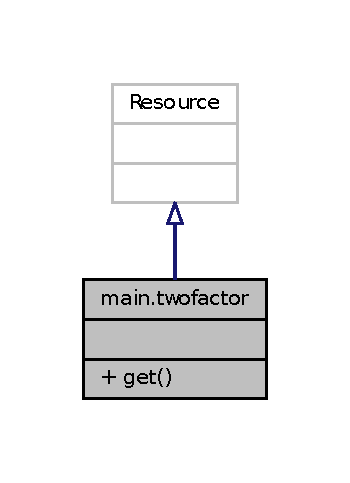
\includegraphics[width=161pt]{classmain_1_1twofactor__inherit__graph}
\end{center}
\end{figure}


Collaboration diagram for main.\+twofactor\+:\nopagebreak
\begin{figure}[H]
\begin{center}
\leavevmode
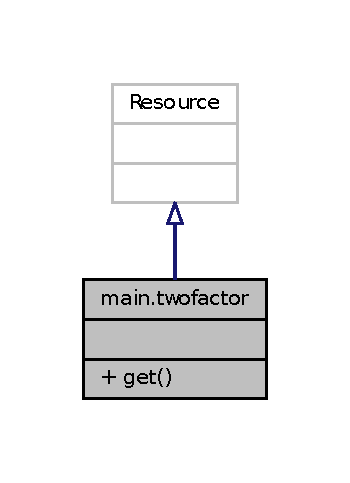
\includegraphics[width=161pt]{classmain_1_1twofactor__coll__graph}
\end{center}
\end{figure}
\doxysubsection*{Public Member Functions}
\begin{DoxyCompactItemize}
\item 
def \mbox{\hyperlink{classmain_1_1twofactor_a87a3b360a2540681f4620d2820f8bb31}{get}} (self)
\end{DoxyCompactItemize}


\doxysubsection{Detailed Description}


Definition at line 124 of file main.\+py.



\doxysubsection{Member Function Documentation}
\mbox{\Hypertarget{classmain_1_1twofactor_a87a3b360a2540681f4620d2820f8bb31}\label{classmain_1_1twofactor_a87a3b360a2540681f4620d2820f8bb31}} 
\index{main.twofactor@{main.twofactor}!get@{get}}
\index{get@{get}!main.twofactor@{main.twofactor}}
\doxysubsubsection{\texorpdfstring{get()}{get()}}
{\footnotesize\ttfamily def main.\+twofactor.\+get (\begin{DoxyParamCaption}\item[{}]{self }\end{DoxyParamCaption})}



Definition at line 125 of file main.\+py.


\begin{DoxyCode}{0}
\DoxyCodeLine{125     \textcolor{keyword}{def }get(self):}
\DoxyCodeLine{126         \textcolor{keywordflow}{if} \textcolor{stringliteral}{'username'} \textcolor{keywordflow}{not} \textcolor{keywordflow}{in} session:}
\DoxyCodeLine{127             \textcolor{keywordflow}{return} redirect(url\_for(\textcolor{stringliteral}{'index'}))}
\DoxyCodeLine{128 }
\DoxyCodeLine{129         user = User.query.filter\_by(username=session[\textcolor{stringliteral}{'username'}]).first()}
\DoxyCodeLine{130 }
\DoxyCodeLine{131         \textcolor{keywordflow}{if} user \textcolor{keywordflow}{is} \textcolor{keywordtype}{None}:}
\DoxyCodeLine{132             \textcolor{keywordflow}{return} redirect(url\_for(\textcolor{stringliteral}{'index'}))}
\DoxyCodeLine{133 }
\DoxyCodeLine{134         param = \{\textcolor{stringliteral}{'Cache-\/Control'}: \textcolor{stringliteral}{'no-\/cache, no-\/store, must-\/revalidate'}, \textcolor{stringliteral}{'Pragma'}: \textcolor{stringliteral}{'no-\/cache'}, \textcolor{stringliteral}{'Expires'}: \textcolor{stringliteral}{'0'}\}}
\DoxyCodeLine{135         response = make\_response(render\_template(\textcolor{stringliteral}{'two-\/factor-\/setup.html'}), 200, param)}
\DoxyCodeLine{136         \textcolor{keywordflow}{return} response}
\DoxyCodeLine{137 }

\end{DoxyCode}


The documentation for this class was generated from the following file\+:\begin{DoxyCompactItemize}
\item 
example/\mbox{\hyperlink{main_8py}{main.\+py}}\end{DoxyCompactItemize}

\hypertarget{classmain_1_1User}{}\section{main.\+User Class Reference}
\label{classmain_1_1User}\index{main.\+User@{main.\+User}}


Inheritance diagram for main.\+User\+:
\nopagebreak
\begin{figure}[H]
\begin{center}
\leavevmode
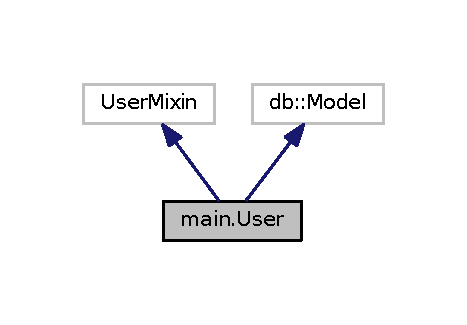
\includegraphics[width=224pt]{classmain_1_1User__inherit__graph}
\end{center}
\end{figure}


Collaboration diagram for main.\+User\+:
\nopagebreak
\begin{figure}[H]
\begin{center}
\leavevmode
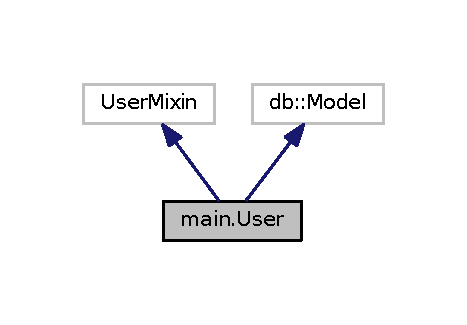
\includegraphics[width=224pt]{classmain_1_1User__coll__graph}
\end{center}
\end{figure}
\subsection*{Public Member Functions}
\begin{DoxyCompactItemize}
\item 
def \hyperlink{classmain_1_1User_ad8e260b3a15f0c0e77c7df7a68d8fcc7}{\+\_\+\+\_\+init\+\_\+\+\_\+} (self, kwargs)
\item 
def \hyperlink{classmain_1_1User_a0086c67911212cc60a39df0424fff2f8}{password} (self)
\item 
def \hyperlink{classmain_1_1User_a5fac9e642b0afaee7e29ddb94e2f1c3e}{password} (self, password)
\item 
def \hyperlink{classmain_1_1User_a8acfe5aa75f7a958346bcb2d156586d9}{verify\+\_\+password} (self, \hyperlink{classmain_1_1User_a0086c67911212cc60a39df0424fff2f8}{password})
\item 
def \hyperlink{classmain_1_1User_a147049a30fbe51d6192d320aa3ea5409}{verify\+\_\+loginhashblock} (self, \hyperlink{classmain_1_1User_aece6256cb85b54493c6d05185f112716}{Login\+HB})
\item 
def \hyperlink{classmain_1_1User_a8b69af8d948dbe7698c904bf94c6ac21}{get\+\_\+totp\+\_\+uri} (self)
\item 
def \hyperlink{classmain_1_1User_a390f1500b4c2fe34d0ba3cf8d1d54906}{verify\+\_\+totp} (self, token)
\end{DoxyCompactItemize}
\subsection*{Static Public Attributes}
\begin{DoxyCompactItemize}
\item 
\hyperlink{classmain_1_1User_af213bc1240b634425b1b571d6bccc561}{id} = db.\+Column(db.\+Integer, primary\+\_\+key=True)
\item 
\hyperlink{classmain_1_1User_afc469a49c408f90fb653d979d2669f62}{username} = db.\+Column(db.\+String(64), \hyperlink{classmain_1_1index}{index}=True)
\item 
\hyperlink{classmain_1_1User_a4bd5dd61d9eca670b326c87ec7f79f94}{password\+\_\+hash} = db.\+Column(db.\+String(128))
\item 
\hyperlink{classmain_1_1User_a2a7a2d67099632b248ad93661e9733d2}{otp\+\_\+secret} = db.\+Column(db.\+String(16))
\item 
\hyperlink{classmain_1_1User_aa3b839482f4a293703c22ae82e9c639d}{Lhashblock} = db.\+Column(db.\+String(128))
\item 
\hyperlink{classmain_1_1User_aece6256cb85b54493c6d05185f112716}{Login\+HB} = str(\hyperlink{classmain_1_1User_aa3b839482f4a293703c22ae82e9c639d}{Lhashblock})
\end{DoxyCompactItemize}


\subsection{Detailed Description}
\begin{DoxyVerb}User model.\end{DoxyVerb}
 

Definition at line 44 of file main.\+py.



\subsection{Constructor \& Destructor Documentation}
\index{main\+::\+User@{main\+::\+User}!\+\_\+\+\_\+init\+\_\+\+\_\+@{\+\_\+\+\_\+init\+\_\+\+\_\+}}
\index{\+\_\+\+\_\+init\+\_\+\+\_\+@{\+\_\+\+\_\+init\+\_\+\+\_\+}!main\+::\+User@{main\+::\+User}}
\subsubsection[{\texorpdfstring{\+\_\+\+\_\+init\+\_\+\+\_\+(self, kwargs)}{__init__(self, kwargs)}}]{\setlength{\rightskip}{0pt plus 5cm}def main.\+User.\+\_\+\+\_\+init\+\_\+\+\_\+ (
\begin{DoxyParamCaption}
\item[{}]{self, }
\item[{}]{kwargs}
\end{DoxyParamCaption}
)}\hypertarget{classmain_1_1User_ad8e260b3a15f0c0e77c7df7a68d8fcc7}{}\label{classmain_1_1User_ad8e260b3a15f0c0e77c7df7a68d8fcc7}


Definition at line 54 of file main.\+py.


\begin{DoxyCode}
54     \textcolor{keyword}{def }\hyperlink{classmain_1_1User_ad8e260b3a15f0c0e77c7df7a68d8fcc7}{\_\_init\_\_}(self, **kwargs):
55         super(User, self).\hyperlink{classmain_1_1User_ad8e260b3a15f0c0e77c7df7a68d8fcc7}{\_\_init\_\_}(**kwargs)
56         \textcolor{keywordflow}{if} self.\hyperlink{classmain_1_1User_a2a7a2d67099632b248ad93661e9733d2}{otp\_secret} \textcolor{keywordflow}{is} \textcolor{keywordtype}{None}:
57             \textcolor{comment}{# generate a random secret}
58             self.\hyperlink{classmain_1_1User_a2a7a2d67099632b248ad93661e9733d2}{otp\_secret} = base64.b32encode(os.urandom(10)).decode(\textcolor{stringliteral}{'utf-8'})
59 
\end{DoxyCode}


\subsection{Member Function Documentation}
\index{main\+::\+User@{main\+::\+User}!get\+\_\+totp\+\_\+uri@{get\+\_\+totp\+\_\+uri}}
\index{get\+\_\+totp\+\_\+uri@{get\+\_\+totp\+\_\+uri}!main\+::\+User@{main\+::\+User}}
\subsubsection[{\texorpdfstring{get\+\_\+totp\+\_\+uri(self)}{get_totp_uri(self)}}]{\setlength{\rightskip}{0pt plus 5cm}def main.\+User.\+get\+\_\+totp\+\_\+uri (
\begin{DoxyParamCaption}
\item[{}]{self}
\end{DoxyParamCaption}
)}\hypertarget{classmain_1_1User_a8b69af8d948dbe7698c904bf94c6ac21}{}\label{classmain_1_1User_a8b69af8d948dbe7698c904bf94c6ac21}


Definition at line 75 of file main.\+py.


\begin{DoxyCode}
75     \textcolor{keyword}{def }\hyperlink{classmain_1_1User_a8b69af8d948dbe7698c904bf94c6ac21}{get\_totp\_uri}(self):
76         \textcolor{keywordflow}{return} \textcolor{stringliteral}{'otpauth://totp/2FA-Demo:\{0\}?secret=\{1\}&issuer=2FA-Demo'}.format(self.
      \hyperlink{classmain_1_1User_afc469a49c408f90fb653d979d2669f62}{username}, self.\hyperlink{classmain_1_1User_a2a7a2d67099632b248ad93661e9733d2}{otp\_secret})
77 
\end{DoxyCode}
\index{main\+::\+User@{main\+::\+User}!password@{password}}
\index{password@{password}!main\+::\+User@{main\+::\+User}}
\subsubsection[{\texorpdfstring{password(self)}{password(self)}}]{\setlength{\rightskip}{0pt plus 5cm}def main.\+User.\+password (
\begin{DoxyParamCaption}
\item[{}]{self}
\end{DoxyParamCaption}
)}\hypertarget{classmain_1_1User_a0086c67911212cc60a39df0424fff2f8}{}\label{classmain_1_1User_a0086c67911212cc60a39df0424fff2f8}


Definition at line 61 of file main.\+py.


\begin{DoxyCode}
61     \textcolor{keyword}{def }\hyperlink{classmain_1_1User_a0086c67911212cc60a39df0424fff2f8}{password}(self):
62         \textcolor{keywordflow}{raise} AttributeError(\textcolor{stringliteral}{'password is not a readable attribute'})
63 
\end{DoxyCode}


Here is the caller graph for this function\+:\nopagebreak
\begin{figure}[H]
\begin{center}
\leavevmode
\includegraphics[width=342pt]{classmain_1_1User_a0086c67911212cc60a39df0424fff2f8_icgraph}
\end{center}
\end{figure}


\index{main\+::\+User@{main\+::\+User}!password@{password}}
\index{password@{password}!main\+::\+User@{main\+::\+User}}
\subsubsection[{\texorpdfstring{password(self, password)}{password(self, password)}}]{\setlength{\rightskip}{0pt plus 5cm}def main.\+User.\+password (
\begin{DoxyParamCaption}
\item[{}]{self, }
\item[{}]{password}
\end{DoxyParamCaption}
)}\hypertarget{classmain_1_1User_a5fac9e642b0afaee7e29ddb94e2f1c3e}{}\label{classmain_1_1User_a5fac9e642b0afaee7e29ddb94e2f1c3e}


Definition at line 65 of file main.\+py.


\begin{DoxyCode}
65     \textcolor{keyword}{def }\hyperlink{classmain_1_1User_a0086c67911212cc60a39df0424fff2f8}{password}(self, password):
66         self.\hyperlink{classmain_1_1User_a4bd5dd61d9eca670b326c87ec7f79f94}{password\_hash} = generate\_password\_hash(password)
67 
\end{DoxyCode}


Here is the call graph for this function\+:\nopagebreak
\begin{figure}[H]
\begin{center}
\leavevmode
\includegraphics[width=342pt]{classmain_1_1User_a5fac9e642b0afaee7e29ddb94e2f1c3e_cgraph}
\end{center}
\end{figure}


\index{main\+::\+User@{main\+::\+User}!verify\+\_\+loginhashblock@{verify\+\_\+loginhashblock}}
\index{verify\+\_\+loginhashblock@{verify\+\_\+loginhashblock}!main\+::\+User@{main\+::\+User}}
\subsubsection[{\texorpdfstring{verify\+\_\+loginhashblock(self, Login\+H\+B)}{verify_loginhashblock(self, LoginHB)}}]{\setlength{\rightskip}{0pt plus 5cm}def main.\+User.\+verify\+\_\+loginhashblock (
\begin{DoxyParamCaption}
\item[{}]{self, }
\item[{}]{Login\+HB}
\end{DoxyParamCaption}
)}\hypertarget{classmain_1_1User_a147049a30fbe51d6192d320aa3ea5409}{}\label{classmain_1_1User_a147049a30fbe51d6192d320aa3ea5409}


Definition at line 71 of file main.\+py.


\begin{DoxyCode}
71     \textcolor{keyword}{def }\hyperlink{classmain_1_1User_a147049a30fbe51d6192d320aa3ea5409}{verify\_loginhashblock}(self, LoginHB):
72         loginhashblock = self.Lhashblock.split(\textcolor{stringliteral}{','})
73         \textcolor{keywordflow}{return} \textcolor{keyword}{True}
74 
\end{DoxyCode}
\index{main\+::\+User@{main\+::\+User}!verify\+\_\+password@{verify\+\_\+password}}
\index{verify\+\_\+password@{verify\+\_\+password}!main\+::\+User@{main\+::\+User}}
\subsubsection[{\texorpdfstring{verify\+\_\+password(self, password)}{verify_password(self, password)}}]{\setlength{\rightskip}{0pt plus 5cm}def main.\+User.\+verify\+\_\+password (
\begin{DoxyParamCaption}
\item[{}]{self, }
\item[{}]{password}
\end{DoxyParamCaption}
)}\hypertarget{classmain_1_1User_a8acfe5aa75f7a958346bcb2d156586d9}{}\label{classmain_1_1User_a8acfe5aa75f7a958346bcb2d156586d9}


Definition at line 68 of file main.\+py.


\begin{DoxyCode}
68     \textcolor{keyword}{def }\hyperlink{classmain_1_1User_a8acfe5aa75f7a958346bcb2d156586d9}{verify\_password}(self, password):
69         \textcolor{keywordflow}{return} check\_password\_hash(self.\hyperlink{classmain_1_1User_a4bd5dd61d9eca670b326c87ec7f79f94}{password\_hash}, password)
70 
\end{DoxyCode}
\index{main\+::\+User@{main\+::\+User}!verify\+\_\+totp@{verify\+\_\+totp}}
\index{verify\+\_\+totp@{verify\+\_\+totp}!main\+::\+User@{main\+::\+User}}
\subsubsection[{\texorpdfstring{verify\+\_\+totp(self, token)}{verify_totp(self, token)}}]{\setlength{\rightskip}{0pt plus 5cm}def main.\+User.\+verify\+\_\+totp (
\begin{DoxyParamCaption}
\item[{}]{self, }
\item[{}]{token}
\end{DoxyParamCaption}
)}\hypertarget{classmain_1_1User_a390f1500b4c2fe34d0ba3cf8d1d54906}{}\label{classmain_1_1User_a390f1500b4c2fe34d0ba3cf8d1d54906}


Definition at line 78 of file main.\+py.


\begin{DoxyCode}
78     \textcolor{keyword}{def }\hyperlink{classmain_1_1User_a390f1500b4c2fe34d0ba3cf8d1d54906}{verify\_totp}(self, token):
79         \textcolor{keywordflow}{return} onetimepass.valid\_totp(token, self.\hyperlink{classmain_1_1User_a2a7a2d67099632b248ad93661e9733d2}{otp\_secret})
80 
81 @lm.user\_loader
\end{DoxyCode}


\subsection{Member Data Documentation}
\index{main\+::\+User@{main\+::\+User}!id@{id}}
\index{id@{id}!main\+::\+User@{main\+::\+User}}
\subsubsection[{\texorpdfstring{id}{id}}]{\setlength{\rightskip}{0pt plus 5cm}main.\+User.\+id = db.\+Column(db.\+Integer, primary\+\_\+key=True)\hspace{0.3cm}{\ttfamily [static]}}\hypertarget{classmain_1_1User_af213bc1240b634425b1b571d6bccc561}{}\label{classmain_1_1User_af213bc1240b634425b1b571d6bccc561}


Definition at line 47 of file main.\+py.

\index{main\+::\+User@{main\+::\+User}!Lhashblock@{Lhashblock}}
\index{Lhashblock@{Lhashblock}!main\+::\+User@{main\+::\+User}}
\subsubsection[{\texorpdfstring{Lhashblock}{Lhashblock}}]{\setlength{\rightskip}{0pt plus 5cm}main.\+User.\+Lhashblock = db.\+Column(db.\+String(128))\hspace{0.3cm}{\ttfamily [static]}}\hypertarget{classmain_1_1User_aa3b839482f4a293703c22ae82e9c639d}{}\label{classmain_1_1User_aa3b839482f4a293703c22ae82e9c639d}


Definition at line 51 of file main.\+py.

\index{main\+::\+User@{main\+::\+User}!Login\+HB@{Login\+HB}}
\index{Login\+HB@{Login\+HB}!main\+::\+User@{main\+::\+User}}
\subsubsection[{\texorpdfstring{Login\+HB}{LoginHB}}]{\setlength{\rightskip}{0pt plus 5cm}main.\+User.\+Login\+HB = str({\bf Lhashblock})\hspace{0.3cm}{\ttfamily [static]}}\hypertarget{classmain_1_1User_aece6256cb85b54493c6d05185f112716}{}\label{classmain_1_1User_aece6256cb85b54493c6d05185f112716}


Definition at line 52 of file main.\+py.

\index{main\+::\+User@{main\+::\+User}!otp\+\_\+secret@{otp\+\_\+secret}}
\index{otp\+\_\+secret@{otp\+\_\+secret}!main\+::\+User@{main\+::\+User}}
\subsubsection[{\texorpdfstring{otp\+\_\+secret}{otp_secret}}]{\setlength{\rightskip}{0pt plus 5cm}main.\+User.\+otp\+\_\+secret = db.\+Column(db.\+String(16))\hspace{0.3cm}{\ttfamily [static]}}\hypertarget{classmain_1_1User_a2a7a2d67099632b248ad93661e9733d2}{}\label{classmain_1_1User_a2a7a2d67099632b248ad93661e9733d2}


Definition at line 50 of file main.\+py.

\index{main\+::\+User@{main\+::\+User}!password\+\_\+hash@{password\+\_\+hash}}
\index{password\+\_\+hash@{password\+\_\+hash}!main\+::\+User@{main\+::\+User}}
\subsubsection[{\texorpdfstring{password\+\_\+hash}{password_hash}}]{\setlength{\rightskip}{0pt plus 5cm}main.\+User.\+password\+\_\+hash = db.\+Column(db.\+String(128))\hspace{0.3cm}{\ttfamily [static]}}\hypertarget{classmain_1_1User_a4bd5dd61d9eca670b326c87ec7f79f94}{}\label{classmain_1_1User_a4bd5dd61d9eca670b326c87ec7f79f94}


Definition at line 49 of file main.\+py.

\index{main\+::\+User@{main\+::\+User}!username@{username}}
\index{username@{username}!main\+::\+User@{main\+::\+User}}
\subsubsection[{\texorpdfstring{username}{username}}]{\setlength{\rightskip}{0pt plus 5cm}main.\+User.\+username = db.\+Column(db.\+String(64), {\bf index}=True)\hspace{0.3cm}{\ttfamily [static]}}\hypertarget{classmain_1_1User_afc469a49c408f90fb653d979d2669f62}{}\label{classmain_1_1User_afc469a49c408f90fb653d979d2669f62}


Definition at line 48 of file main.\+py.



The documentation for this class was generated from the following file\+:\begin{DoxyCompactItemize}
\item 
example/\hyperlink{main_8py}{main.\+py}\end{DoxyCompactItemize}

\chapter{File Documentation}
\hypertarget{config_8py}{}\doxysection{example/config.py File Reference}
\label{config_8py}\index{example/config.py@{example/config.py}}
\doxysubsection*{Namespaces}
\begin{DoxyCompactItemize}
\item 
 \mbox{\hyperlink{namespaceconfig}{config}}
\end{DoxyCompactItemize}
\doxysubsection*{Variables}
\begin{DoxyCompactItemize}
\item 
string \mbox{\hyperlink{namespaceconfig_a9a12d1637d39ac73154cfb736dd2e36a}{config.\+S\+E\+C\+R\+E\+T\+\_\+\+K\+EY}} = \textquotesingle{}top-\/secret\textquotesingle{}
\item 
\mbox{\hyperlink{namespaceconfig_abfb380a150ba49f3296981414777eed8}{config.\+S\+Q\+L\+A\+L\+C\+H\+E\+M\+Y\+\_\+\+D\+A\+T\+A\+B\+A\+S\+E\+\_\+\+U\+RI}} = os.\+environ.\+get(\textquotesingle{}D\+A\+T\+A\+B\+A\+S\+E\+\_\+\+U\+RL\textquotesingle{}, \textquotesingle{}sqlite\+:///db.\+sqlite\textquotesingle{})
\item 
bool \mbox{\hyperlink{namespaceconfig_af3c11aea509436fc561e22b8a479f7b3}{config.\+S\+Q\+L\+A\+L\+C\+H\+E\+M\+Y\+\_\+\+T\+R\+A\+C\+K\+\_\+\+M\+O\+D\+I\+F\+I\+C\+A\+T\+I\+O\+NS}} = False
\end{DoxyCompactItemize}

\hypertarget{main_8py}{}\section{example/main.py File Reference}
\label{main_8py}\index{example/main.\+py@{example/main.\+py}}
\subsection*{Classes}
\begin{DoxyCompactItemize}
\item 
class \hyperlink{classmain_1_1User}{main.\+User}
\item 
class \hyperlink{classmain_1_1RegisterForm}{main.\+Register\+Form}
\item 
class \hyperlink{classmain_1_1index}{main.\+index}
\item 
class \hyperlink{classmain_1_1register}{main.\+register}
\item 
class \hyperlink{classmain_1_1twofactor}{main.\+twofactor}
\item 
class \hyperlink{classmain_1_1qrcode}{main.\+qrcode}
\item 
class \hyperlink{classmain_1_1login}{main.\+login}
\item 
class \hyperlink{classmain_1_1logout}{main.\+logout}
\item 
class \hyperlink{classmain_1_1command}{main.\+command}
\end{DoxyCompactItemize}
\subsection*{Namespaces}
\begin{DoxyCompactItemize}
\item 
 \hyperlink{namespacemain}{main}
\end{DoxyCompactItemize}
\subsection*{Functions}
\begin{DoxyCompactItemize}
\item 
def \hyperlink{namespacemain_a64310d76bee3c7581aaa85925bf1bb53}{main.\+load\+\_\+user} (user\+\_\+id)
\item 
def \hyperlink{namespacemain_a0803c7dc3e1c168a3fbcf5b054109aa1}{main.\+not\+\_\+found} (e)
\end{DoxyCompactItemize}
\subsection*{Variables}
\begin{DoxyCompactItemize}
\item 
bool \hyperlink{namespacemain_ad2cce3c3d1036d38f161e4814c97e1b5}{main.\+D\+E\+B\+UG} = False
\item 
\hyperlink{namespacemain_a5fa94f0581009434c7a63791944d6ff4}{main.\+app} = Flask(\+\_\+\+\_\+name\+\_\+\+\_\+)
\item 
\hyperlink{namespacemain_a2f0b4b807236469879d595c7f18850aa}{main.\+api} = Api(app)
\item 
\hyperlink{namespacemain_aad5fb0badb72b68b03eda5bc7e72f989}{main.\+minutes}
\item 
\hyperlink{namespacemain_a2799db3c64165e5659fada6c15d90aea}{main.\+bootstrap} = Bootstrap(app)
\item 
\hyperlink{namespacemain_afadee2a30284fe18a4fee574c23c94e3}{main.\+db} = S\+Q\+L\+Alchemy(app)
\item 
\hyperlink{namespacemain_aaf584fa2bbd608ba30fe2a84f4a6e604}{main.\+lm} = Login\+Manager(app)
\end{DoxyCompactItemize}

\hypertarget{run_8py}{}\section{example/run.py File Reference}
\label{run_8py}\index{example/run.\+py@{example/run.\+py}}
\subsection*{Namespaces}
\begin{DoxyCompactItemize}
\item 
 \hyperlink{namespacerun}{run}
\end{DoxyCompactItemize}
\subsection*{Variables}
\begin{DoxyCompactItemize}
\item 
\hyperlink{namespacerun_a24785e11198aac41f0051e51857331aa}{run.\+debug}
\item 
\hyperlink{namespacerun_af7767eb404b922097d7206695c016bad}{run.\+host} = os.\+environ.\+get(\textquotesingle{}IP\textquotesingle{}, \textquotesingle{}0.\+0.\+0.\+0\textquotesingle{})
\item 
\hyperlink{namespacerun_a7a6a5c33b9e900b36c2b941d5212210e}{run.\+port} = int(os.\+environ.\+get(\textquotesingle{}P\+O\+RT\textquotesingle{}, 80))
\end{DoxyCompactItemize}

\hypertarget{loginhashblock_8py}{}\section{loginhashblock/loginhashblock.py File Reference}
\label{loginhashblock_8py}\index{loginhashblock/loginhashblock.\+py@{loginhashblock/loginhashblock.\+py}}
\subsection*{Namespaces}
\begin{DoxyCompactItemize}
\item 
 \hyperlink{namespaceloginhashblock}{loginhashblock}
\end{DoxyCompactItemize}
\subsection*{Functions}
\begin{DoxyCompactItemize}
\item 
def \hyperlink{namespaceloginhashblock_af47615d0e87d554eae9e6d49131fe49c}{loginhashblock.\+print\+\_\+\+L\+H\+Blist} (L\+H\+Bliststr, D\+E\+B\+UG=False)
\item 
def \hyperlink{namespaceloginhashblock_a104d0a92cdfb6c337794b6ded42667d4}{loginhashblock.\+pbkdf2\+\_\+hash} (data, salt, iterations, dklen=None, hash\+\_\+name=\char`\"{}sha256\char`\"{}, D\+E\+B\+UG=False)
\item 
def \hyperlink{namespaceloginhashblock_afe116dea3aaff238a5fa2bcd6edf2281}{loginhashblock.\+create\+\_\+salt} (length, R\+A\+N\+D\+\_\+\+C\+H\+A\+RS=None, D\+E\+B\+UG=False)
\item 
def \hyperlink{namespaceloginhashblock_ab3608ba58ffedb0bd8bba86ce71fdefe}{loginhashblock.\+create\+\_\+loginhashblocklist} (prev\+\_\+\+L\+H\+Blist\+Str, D\+E\+B\+UG=D\+E\+B\+UG)
\item 
def \hyperlink{namespaceloginhashblock_a7baa4021b9f57044f8227c2e0320ee2b}{loginhashblock.\+update\+\_\+loginhashblocklist} (L\+H\+Blist\+Str, prev\+\_\+\+L\+HB, D\+E\+B\+UG=False)
\item 
def \hyperlink{namespaceloginhashblock_a935d8ae1c51e50f9e5db6a1d5f02b1b8}{loginhashblock.\+create\+\_\+hash} (salt, target, hash\+\_\+name=\char`\"{}sha256\char`\"{}, iterations=100000, kdf=None, D\+E\+B\+UG=False)
\item 
def \hyperlink{namespaceloginhashblock_ac7faa165bc305e611390727f11946424}{loginhashblock.\+valid\+\_\+hash} (target\+\_\+hash, salt, target, method, D\+E\+B\+UG=False)
\item 
def \hyperlink{namespaceloginhashblock_a1908d7c90a7ea1a7f84eeac3a1378b57}{loginhashblock.\+get\+\_\+device\+Id} (loginhashblock, D\+E\+B\+UG=False)
\item 
def \hyperlink{namespaceloginhashblock_a1bd31fe2f0ea4e6673127d72b6c42826}{loginhashblock.\+create\+\_\+device\+Id} (D\+E\+B\+UG=False)
\item 
def \hyperlink{namespaceloginhashblock_ac24dd842eb90e0ede55e842d44148d5b}{loginhashblock.\+compare\+\_\+loginhashblock} (a, b, D\+E\+B\+UG=False)
\item 
def \hyperlink{namespaceloginhashblock_ac120dd8384bd51c357e2ad5f6cb2f99a}{loginhashblock.\+valid\+\_\+loginhashblock} (loginhashblock, D\+E\+B\+UG=False)
\item 
def \hyperlink{namespaceloginhashblock_ab6bafe3dab103cc698822367e53d4a64}{loginhashblock.\+update\+\_\+loginhashblock} (prev\+\_\+loginhashblock, D\+E\+B\+UG=False)
\item 
def \hyperlink{namespaceloginhashblock_a978cb4557443cefddac883f3d92ad8e1}{loginhashblock.\+is\+Registed\+L\+HB} (client\+\_\+loginhashblock, L\+H\+Bliststr, D\+E\+B\+UG=False)
\item 
def \hyperlink{namespaceloginhashblock_ab2ceb1d30aad9af290ac7d44e9f95bf2}{loginhashblock.\+get\+\_\+loginhashblock} (devid, loginhashblocklist, D\+E\+B\+UG=False)
\item 
def \hyperlink{namespaceloginhashblock_ad3ef8dab740c69ca8424797f9c146a53}{loginhashblock.\+create\+\_\+loginhashblock} (devid, key=None, D\+E\+B\+UG=False)
\end{DoxyCompactItemize}
\subsection*{Variables}
\begin{DoxyCompactItemize}
\item 
bool \hyperlink{namespaceloginhashblock_ad198a2ffc3d7bab32167aed00d2f5c65}{loginhashblock.\+D\+E\+B\+UG} = False
\end{DoxyCompactItemize}

\hypertarget{unittest_8py}{}\section{loginhashblock/unittest.py File Reference}
\label{unittest_8py}\index{loginhashblock/unittest.\+py@{loginhashblock/unittest.\+py}}
\subsection*{Classes}
\begin{DoxyCompactItemize}
\item 
class \hyperlink{classunittest_1_1bcolors}{unittest.\+bcolors}
\end{DoxyCompactItemize}
\subsection*{Namespaces}
\begin{DoxyCompactItemize}
\item 
 \hyperlink{namespaceunittest}{unittest}
\end{DoxyCompactItemize}
\subsection*{Functions}
\begin{DoxyCompactItemize}
\item 
def \hyperlink{namespaceunittest_a217a1a3af5bc9748f2f6194bf79402bc}{unittest.\+unittest\+\_\+print} (message)
\item 
def \hyperlink{namespaceunittest_a642ec5401fe406315f1489d237ba826e}{unittest.\+unittest\+\_\+title\+\_\+print} (message)
\item 
def \hyperlink{namespaceunittest_a9e16eaba67b93461be6ea8ef6332507a}{unittest.\+unittest\+\_\+update\+\_\+loginhashblocklist} ()
\item 
def \hyperlink{namespaceunittest_a0e10bea14aac2cc6a08d76f422b9328d}{unittest.\+unittest\+\_\+create\+\_\+loginhashblocklist} ()
\item 
def \hyperlink{namespaceunittest_aa1c9f3b8631f7f60770414cf8958e2be}{unittest.\+unittest\+\_\+request\+\_\+login\+\_\+token} ()
\item 
def \hyperlink{namespaceunittest_a8b30a1b14f91e9e9d093c13a7e68ee93}{unittest.\+unittest\+\_\+request\+\_\+login\+\_\+notoken} ()
\item 
def \hyperlink{namespaceunittest_afeccd95cc658ca5f2ffb4df7a1edbbd2}{unittest.\+mok\+\_\+request\+\_\+post} (token, prev\+\_\+\+L\+HB, verify\+\_\+totp, L\+H\+Blist\+Str)
\end{DoxyCompactItemize}
\subsection*{Variables}
\begin{DoxyCompactItemize}
\item 
bool \hyperlink{namespaceunittest_a6f95c254ae4668ea73efe6cf7ca3c36d}{unittest.\+D\+E\+B\+UG} = False
\end{DoxyCompactItemize}

%--- End generated contents ---

% Index
\backmatter
\newpage
\phantomsection
\clearemptydoublepage
\addcontentsline{toc}{chapter}{Index}
\printindex

\end{document}
